%!TEX TS-program = xelatex

%!TEX root = ../Thesis.tex

% This information is used in titlepage, colophon, preface and hyperref setup (pdf metainfo), and other options.

%\def\thesistypeabbr{B.Eng.}
%\def\thesistype    {Bachelor of Engineering}
%\def\thesistypeabbr{B.Sc.Eng.}
%\def\thesistype    {Bachelor of Science in Engineering}
\def\thesistypeabbr{M.Sc.}
\def\thesistype    {Master of Science in Engineering}
%\def\thesistypeabbr{Ph.D.}
%\def\thesistype    {Doctor of Philosophy}

\def\thesisauthor  {Mads Esben Hansen (s174434)}
\def\thesistitle   {Take-home Exam 02686}
\def\thesissubtitle{Scientific Computing for Differential Equations}
\def\thesislocation{Kongens Lyngby}

\def\papersize{b5paper} % Final papersize (b5paper/a4paper), recommended papersize for DTU Compute is b5paper
\def\showtrims{false}   % Print on larger paper than \papersize and show trim marks (true/false)?

\def\showtodos    {true}  % Show todos (true/false)?
\def\confidential {false} % Confidential thesis (true/false)?

%!TEX root = ../Thesis.tex
\RequirePackage[l2tabu,orthodox]{nag} % Old habits die hard
\RequirePackage{pdftexcmds}

\newcommand{\papersizeswitch}[3]{\ifnum\pdfstrcmp{\papersize}{#1}=0#2\else#3\fi}
\papersizeswitch{b5paper}{\def\classfontsize{10pt}}{\def\classfontsize{12pt}}
\documentclass[\classfontsize,\papersize,twoside,showtrims,extrafontsizes]{memoir}
%!TEX root = ../Thesis.tex
\RequireXeTeX

\showtrimsoff
\papersizeswitch{b5paper}{
    % Stock and paper layout
    \pagebv
    \setlrmarginsandblock{26mm}{20mm}{*}
    \setulmarginsandblock{35mm}{30mm}{*}
    \setheadfoot{8mm}{10mm}
    \setlength{\headsep}{7mm}
    \setlength{\marginparwidth}{18mm}
    \setlength{\marginparsep}{2mm}
}{
    \papersizeswitch{a4paper}{
        \pageaiv
        \setlength{\trimtop}{0pt}
        \setlength{\trimedge}{\stockwidth}
        \addtolength{\trimedge}{-\paperwidth}
        \settypeblocksize{634pt}{448.13pt}{*}
        \setulmargins{4cm}{*}{*}
        \setlrmargins{*}{*}{0.66}
        \setmarginnotes{17pt}{51pt}{\onelineskip}
        \setheadfoot{\onelineskip}{2\onelineskip}
        \setheaderspaces{*}{2\onelineskip}{*}
    }{
    }
}
\ifnum\pdfstrcmp{\showtrims}{true}=0
    % For printing B5 on A4 with trimmarks
    \showtrimson
    \papersizeswitch{b5paper}{\stockaiv}{\stockaiii}
    \setlength{\trimtop}{\stockheight}
    \addtolength{\trimtop}{-\paperheight}
    \setlength{\trimtop}{0.5\trimtop}
    \setlength{\trimedge}{\stockwidth}
    \addtolength{\trimedge}{-\paperwidth}
    \setlength{\trimedge}{0.5\trimedge}
    
    % bigger todos if trim marks
    \setmarginnotes{10pt}{95pt}{\onelineskip}

    \trimLmarks
    
    % put jobname in left top trim mark
    \renewcommand*{\tmarktl}{%
      \begin{picture}(0,0)
        \unitlength 1mm
        \thinlines
        \put(-2,0){\line(-1,0){18}}
        \put(0,2){\line(0,1){18}}
        \put(3,15){\normalfont\ttfamily\fontsize{8bp}{10bp}\selectfont\jobname\ \
          \today\ \ 
          \printtime\ \ 
          Page \thepage}
      \end{picture}}

    % Remove middle trim marks for cleaner layout
    \renewcommand*{\tmarktm}{}
    \renewcommand*{\tmarkml}{}
    \renewcommand*{\tmarkmr}{}
    \renewcommand*{\tmarkbm}{}
\fi

\checkandfixthelayout                 % Check if errors in paper format!
\sideparmargin{outer}                 % Put sidemargins in outer position (why the fuck is this option not default by the class?)

% Large environments
\usepackage{microtype}
\usepackage{mathtools}
\usepackage{listings}                 % Source code printer for LaTeX
\usepackage{tikz}

% Links
\usepackage[hyphens]{url}             % Allow hyphens in URL's
\usepackage[unicode=false,psdextra]{hyperref}                 % References package

% Graphics and colors
\usepackage{graphicx}                 % Including graphics and using colours
\usepackage{xcolor}                   % Defined more color names
\usepackage{eso-pic}                  % Watermark and other bag
\usepackage{preamble/dtucolors}
\graphicspath{{graphics/}}

% Language
\usepackage{polyglossia}    % multilingual typesetting and appropriate hyphenation
\setdefaultlanguage{english}
\usepackage{csquotes}       % language sensitive quotation facilities

% Floating objets, captions and references
\usepackage{flafter}  % floats is positioned after or where it is defined! 
%\setfloatlocations{figure}{bhtp}   % Set floats for all figures
%\setfloatlocations{table}{bhtp}    % Set floats for all tables
%\setFloatBlockFor{section}         % Typeset floats before each section
\usepackage[noabbrev,nameinlink,capitalise]{cleveref} % Clever references. Options: "fig. !1!" --> "!Figure 1!"
\hangcaption
\captionnamefont{\bfseries}
\subcaptionlabelfont{\bfseries}
\newsubfloat{figure}
\newsubfloat{table}
%\letcountercounter{figure}{table}         % Consecutive table and figure numbering
%\letcountercounter{lstlisting}{table}     % Consecutive table and listings numbering
\captiontitlefinal{.}
% strip things from equation references, making them "(1)" instead of "Equation~1"
% from http://tex.stackexchange.com/questions/122174/how-to-strip-eq-from-cleveref
\crefformat{equation}{(#2#1#3)}
\crefrangeformat{equation}{(#3#1#4) to~(#5#2#6)}
\crefmultiformat{equation}{(#2#1#3)}%
{ and~(#2#1#3)}{, (#2#1#3)}{ and~(#2#1#3)}

% Table of contents (TOC)
\setcounter{tocdepth}{1}              % Depth of table of content
\setcounter{secnumdepth}{2}           % Depth of section numbering
\setcounter{maxsecnumdepth}{3}        % Max depth of section numbering

% Todos
\usepackage{totcount}                 % For total counting of counters
\def\todoshowing{}
\ifnum\pdfstrcmp{\showtodos}{false}=0
    \def\todoshowing{disable}
\fi
\usepackage[colorinlistoftodos,\todoshowing]{todonotes} % Todonotes package for nice todos
\newtotcounter{todocounter}           % Creates counter in todo
\let\oldtodo\todo
\newcommand*{\newtodo}[2][]{\stepcounter{todocounter}\oldtodo[#1]{\thesection~(\thetodocounter)~#2}}
\let\todo\newtodo
\let\oldmissingfigure\missingfigure
\newcommand*{\newmissingfigure}[2][]{\stepcounter{todocounter}\oldmissingfigure[#1]{\thesection~(\thetodocounter)~#2}}
\let\missingfigure\newmissingfigure
\makeatletter
\newcommand*{\mylistoftodos}{% Only show list if there are todos
\if@todonotes@disabled
\else
    \ifnum\totvalue{todocounter}>0
        \markboth{\@todonotes@todolistname}{\@todonotes@todolistname}
        \phantomsection\todototoc
        \listoftodos
    \else
    \fi
\fi
}
\makeatother
\newcommand{\lesstodo}[2][]{\todo[color=green!40,#1]{#2}}
\newcommand{\moretodo}[2][]{\todo[color=red!40,#1]{#2}}

% Chapterstyle
\makeatletter
\makechapterstyle{mychapterstyle}{
    \chapterstyle{default}
    \def\format{\normalfont\sffamily}

    \setlength\beforechapskip{0mm}

    \renewcommand*{\chapnamefont}{\format\HUGE}
    \renewcommand*{\chapnumfont}{\format\fontsize{54}{54}\selectfont}
    \renewcommand*{\chaptitlefont}{\format\fontsize{42}{42}\selectfont}

    \renewcommand*{\printchaptername}{\chapnamefont\MakeUppercase{\@chapapp}}
    \patchcommand{\printchaptername}{\begingroup\color{dtugray}}{\endgroup}
    \renewcommand*{\chapternamenum}{\space\space}
    \patchcommand{\printchapternum}{\begingroup\color{dtured}}{\endgroup}
    \renewcommand*{\printchapternonum}{%
        \vphantom{\printchaptername\chapternamenum\chapnumfont 1}
        \afterchapternum
    }

    \setlength\midchapskip{1ex}

    \renewcommand*{\printchaptertitle}[1]{\raggedleft \chaptitlefont ##1}
    \renewcommand*{\afterchaptertitle}{\vskip0.5\onelineskip \hrule \vskip1.3\onelineskip}
}
\makeatother
\chapterstyle{mychapterstyle}

% Header and footer
\def\hffont{\sffamily\small}
\makepagestyle{myruled}
\makeheadrule{myruled}{\textwidth}{\normalrulethickness}
\makeevenhead{myruled}{\hffont\thepage}{}{\hffont\leftmark}
\makeoddhead{myruled}{\hffont\rightmark}{}{\hffont\thepage}
\makeevenfoot{myruled}{}{}{}
\makeoddfoot{myruled}{}{}{}
\makepsmarks{myruled}{
    \nouppercaseheads
    \createmark{chapter}{both}{shownumber}{}{\space}
    \createmark{section}{right}{shownumber}{}{\space}
    \createplainmark{toc}{both}{\contentsname}
    \createplainmark{lof}{both}{\listfigurename}
    \createplainmark{lot}{both}{\listtablename}
    \createplainmark{bib}{both}{\bibname}
    \createplainmark{index}{both}{\indexname}
    \createplainmark{glossary}{both}{\glossaryname}
}
\pagestyle{myruled}
\copypagestyle{cleared}{myruled}      % When \cleardoublepage, use myruled instead of empty
\makeevenhead{cleared}{\hffont\thepage}{}{} % Remove leftmark on cleared pages

\makeevenfoot{plain}{}{}{}            % No page number on plain even pages (chapter begin)
\makeoddfoot{plain}{}{}{}             % No page number on plain odd pages (chapter begin)

% \*section, \*paragraph font styles
\setsecheadstyle              {\huge\sffamily\raggedright}
\setsubsecheadstyle           {\LARGE\sffamily\raggedright}
\setsubsubsecheadstyle        {\Large\sffamily\raggedright}
%\setparaheadstyle             {\normalsize\sffamily\itseries\raggedright}
%\setsubparaheadstyle          {\normalsize\sffamily\raggedright}


% Hypersetup
\hypersetup{
    pdfauthor={\thesisauthor{}},
    pdftitle={\thesistitle{}},
    pdfsubject={\thesissubtitle{}},
    pdfdisplaydoctitle,
    bookmarksnumbered=true,
    bookmarksopen,
    breaklinks,
    linktoc=all,
    plainpages=false,
    unicode=true,
    colorlinks=false,
    citebordercolor=dtured,           % color of links to bibliography
    filebordercolor=dtured,           % color of file links
    linkbordercolor=dtured,           % color of internal links (change box color with linkbordercolor)
    urlbordercolor=s13,               % color of external links
    hidelinks,                        % Do not show boxes or colored links.
}
% Hack to make right pdfbookmark link. The normal behavior links just below the chapter title. This hack put the link just above the chapter like any other normal use of \chapter.
% Another solution can be found in http://tex.stackexchange.com/questions/59359/certain-hyperlinks-memoirhyperref-placed-too-low
\makeatletter
\renewcommand{\@memb@bchap}{%
  \ifnobibintoc\else
    \phantomsection
    \addcontentsline{toc}{chapter}{\bibname}%
  \fi
  \chapter*{\bibname}%
  \bibmark
  \prebibhook
}
\let\oldtableofcontents\tableofcontents
\newcommand{\newtableofcontents}{
    \@ifstar{\oldtableofcontents*}{
        \phantomsection\addcontentsline{toc}{chapter}{\contentsname}\oldtableofcontents*}}
\let\tableofcontents\newtableofcontents
\makeatother

% Confidential
\newcommand{\confidentialbox}[1]{
    \put(0,0){\parbox[b][\paperheight]{\paperwidth}{
        \begin{vplace}
            \centering
            \scalebox{1.3}{
                \begin{tikzpicture}
                    \node[very thick,draw=red!#1,color=red!#1,
                          rounded corners=2pt,inner sep=8pt,rotate=-20]
                          {\sffamily \HUGE \MakeUppercase{Confidential}};
                \end{tikzpicture}
            }
        \end{vplace}
    }}
}

% Prefrontmatter
\newcommand{\prefrontmatter}{
    \pagenumbering{alph}
    \ifnum\pdfstrcmp{\confidential}{true}=0
        \AddToShipoutPictureBG{\confidentialbox{10}}   % 10% classified box in background on each page
        \AddToShipoutPictureFG*{\confidentialbox{100}} % 100% classified box in foreground on first page
    \fi
}

% DTU frieze
\newcommand{\frieze}{%
    \AddToShipoutPicture*{
        \put(0,0){
            \parbox[b][\paperheight]{\paperwidth}{%
                
\includegraphics[trim=130mm 0 0 0,width=0.9\textwidth]{DTU-frise-SH-15}
                \vspace*{2.5cm}
            }
        }
    }
}

% This is a double sided book. If there is a last empty page lets use it for some fun e.g. the frieze.
% NB: For a fully functional hack the \clearpage used in \include does some odd thinks with the sequence numbering. Thefore use \input instead of \include at the end of the book. If bibliography is used at last everything should be ok.
\makeatletter
% Adjust so gatherings is allowd for single sheets too! (hacking functions in memoir.dtx)
\patchcmd{\leavespergathering}{\ifnum\@memcnta<\tw@}{\ifnum\@memcnta<\@ne}{
    \leavespergathering{1}
    % Insert the frieze
    \patchcmd{\@memensuresigpages}{\repeat}{\repeat\frieze}{}{}
}{}
\makeatother

%!TEX root = ../Thesis.tex

% Text fonts (http://www.macfreek.nl/memory/Fonts_in_LaTeX)
% Install fonts from /usr/local/texlive/<version>/texmf-dist/fonts/opentype/public
\usepackage{fontspec}

% Sans-serif font
\setsansfont[
    Ligatures=TeX,
    Extension=.otf,
    UprightFont=*-regular,
    BoldFont=*-bold,
    ItalicFont=*-italic,
    BoldItalicFont=*-bolditalic,
    %SlantedFont=,
    %BoldSlantedFont=,
    %SmallCapsFont=
    Scale=0.8      % Adjustmens when using math in sections
]{texgyreadventor}
%\setsansfont[Ligatures=TeX]{Neo Sans Intel}    % Neo Sans Intel – Like DTU font but more symbols
%\setsansfont[
%    Ligatures=TeX,
%    Scale=0.8
%]{NeoSans}           % NeoSans – DTU font (missing `+' symbols and other)
%\setsansfont[Ligatures=TeX]{CMU Sans Serif}    % Computer Modern Unicode font
%\setsansfont[Ligatures=TeX]{Latin Modern Sans} % Latin Modern Sans serif font

% Use this for more convienent sans serif font in math mode.
%\setmathsf{Latin Modern Sans}


%!TEX root = ../Thesis.tex

% Content specific packages.

\usepackage{float}
\usepackage{blindtext}
\usepackage[lined,ruled,linesnumbered,commentsnumbered]{algorithm2e}
\usepackage{tcolorbox}
\usepackage{pgfplots}                 % Plot tools
\usetikzlibrary{
    arrows,
    matrix,
    positioning,
    shapes,
    topaths,
}
\pgfplotsset{compat=1.7}

% Listings
\lstset{
	backgroundcolor=\color{gray!10},  % background color
    basicstyle=\footnotesize\ttfamily,% the size of the fonts that are used for the code
    breakatwhitespace=false,          % sets if automatic breaks should only happen at whitespace
    breaklines=true,                  % sets automatic line breaking
    captionpos=b,                     % sets the caption-position to bottom
    commentstyle=\color{s14a},        % comment style
    deletekeywords={},                % if you want to delete keywords from the given language
    escapeinside={\%*}{*)},           % if you want to add LaTeX within your code
    frame=single,                     % adds a frame around the code
    keywordstyle=\bfseries\ttfamily\color{s09}, % keyword style
    language=Python,                  % the language of the code
    morekeywords={*,...},             % if you want to add more keywords to the set
    numbers=left,                     % where to put the line-numbers; possible values are (none, left, right)
    numbersep=5pt,                    % how far the line-numbers are from the code
    numberstyle=\sffamily\tiny\color{dtugray}, % the style that is used for the line-numbers
    rulecolor=\color{dtugray},        % if not set, the frame-color may be changed on line-breaks within not-black text (e.g. comments (green here))
    showspaces=false,                 % show spaces everywhere adding particular underscores; it overrides 'showstringspaces'
    showstringspaces=false,           % underline spaces within strings only
    showtabs=false,                   % show tabs within strings adding particular underscores
    stepnumber=1,                     % the step between two line-numbers. If it's 1, each line will be numbered
    stringstyle=\color{s07},          % string literal style
    tabsize=2,                        % sets default tabsize to 2 spaces
    title=\lstname,                   % show the filename of files included with \lstinputlisting; also try caption instead of title
}

\usepackage{mcode}


%\usepackage{caption}
%\usepackage{subcaption}




\newcommand{\probP}{\text{I\kern-0.15em P}}
\newcommand{\probE}{\text{I\kern-0.15em E}}
\newcommand{\probR}{\text{I\kern-0.15em R}}
\newcommand{\probV}{\mathbb{V}}
\newcommand{\ind}{\perp\!\!\!\!\perp} 




\begin{document}

\prefrontmatter
%!TEX root = ../Thesis.tex 
\thispagestyle{empty}             % No page numbers
\calccentering{\unitlength}
\begin{adjustwidth*}{\unitlength}{-\unitlength}
    \begin{adjustwidth}{-0.5cm}{-0.5cm}
        \sffamily
        \begin{flushright}
            Take-home Exam\\*[0cm]
            \thesistype{}\\
        \end{flushright}
        \vspace*{\fill}
        \noindent
        
\includegraphics[width=0.75\textwidth]{DTU-Compute-B-UK}\\*[0.5cm]
        \HUGE \thesistitle{}\\*[0.2cm]
        \Huge \thesissubtitle{}\\*[1.2cm]
        \parbox[b]{0.5\linewidth}{%
            \LARGE 
            \thesisauthor{}\\*[1.2cm]
            \Large
            \thesislocation{} \the\year
        }
        \hfill
\includegraphics[scale=0.7]{DTU-logo-CMYK}
    \end{adjustwidth}
\end{adjustwidth*}
\normalfont
\normalsize

%\cleartoevenpage
%%!TEX root = ../Thesis.tex
\thispagestyle{empty} % No page numbers
\frieze
\vspace*{\fill}
\noindent
\sffamily
\small
\textbf{DTU Compute}\\
\textbf{Department of Applied Mathematics and Computer Science}\\
\textbf{Technical University of Denmark}\\
\\
Matematiktorvet\\
Building 303B\\
2800 Kongens Lyngby, Denmark\\
Phone +45 4525 3031\\
compute@compute.dtu.dk\\
www.compute.dtu.dk\\
\normalsize
\normalfont
\vspace*{2.5cm}

%\clearforchapter

%\frontmatter
%%!TEX root = ../Thesis.tex
\chapter{Summary}
Lorem ipsum dolor sit amet, consectetur adipisicing elit, sed do eiusmod tempor incididunt ut labore et dolore magna aliqua. Ut enim ad minim veniam, quis nostrud exercitation ullamco laboris nisi ut aliquip ex ea commodo consequat. Duis aute irure dolor in reprehenderit in voluptate velit esse cillum dolore eu fugiat nulla pariatur. Excepteur sint occaecat cupidatat non proident, sunt in culpa qui officia deserunt mollit anim id est laborum.

%%!TEX root = ../Thesis.tex
\chapter{Preface}
This xxx thesis was prepared at the department of Applied Mathematics and Computer Science at the Technical University of Denmark in fulfillment of the requirements for acquiring a yyy degree in zzz.

\vfill

{
\centering
    \thesislocation{}, \today\\[1cm]
    \hspace{3cm}
\includegraphics[scale=0.4]{Signature}\\[1cm]
\begin{flushright}
    \thesisauthor{}
\end{flushright}
}
%%!TEX root = ../Thesis.tex
\chapter{Acknowledgements}
Lorem ipsum dolor sit amet, consectetur adipisicing elit, sed do eiusmod tempor incididunt ut labore et dolore magna aliqua. Ut enim ad minim veniam, quis nostrud exercitation ullamco laboris nisi ut aliquip ex ea commodo consequat. Duis aute irure dolor in reprehenderit in voluptate velit esse cillum dolore eu fugiat nulla pariatur. Excepteur sint occaecat cupidatat non proident, sunt in culpa qui officia deserunt mollit anim id est laborum.

%\clearforchapter
\tableofcontents
%\clearforchapter
%\mylistoftodos

\mainmatter
%!TEX root = ../Thesis.tex
\chapter*{Introduction}
This report is the take-home exam for the course 02686 (Scientific Computing for Differential Equations) for the spring 2022. 

In mathematics and computational science, an initial value problem (IVP) is a type of value problem where one seeks a solution $y(t)$ of a differential equation in which the unknown function $y$ and its derivatives are evaluated at an initial point $t=a$. The initial conditions consist of a specified function $y(a)$, called the "initial value", and one or more derivatives of this function, all evaluated at the point $t=a$. The existence and uniqueness theorem for IVPs states that under certain conditions on $f$, there exists a unique solution to the IVP defined on some interval containing the point $t=a$.

The Runge–Kutta methods are a family of iterative methods for solving differential equations numerically. They are named after German mathematicians Carl Runge and Martin Kutta, who developed them in 1901. These methods were first applied to practical problems by British mathematician Ernest Rutherford in 1904–1905 while he was working on his doctoral thesis at Cambridge University under Joseph Larmor.

We will in this report discuss how to categorize the numerical methods, specifically in relation to their \textit{order} and \textit{stability}. We will test \textit{explicit} and \textit{implicit} Runge Kutta methods. Mostly in relation to IVPs, however, we will also address the topic of stochastic differential equations (SDEs). Specifically, we will address explicit Euler, implicit Euler, classical Runge Kutta, Dormand-prince5(4) and ESDIRK23 for IVPs, and explicit-explicit and implicit-explicit methods for SDEs. We will test the methods on real problems and discuss the results. 

Throughout the report we will implement the methods discussed Matlab and display the code. Additionally, we will call the code using a \textit{wrapper}, such that all methods will have a similar easy-to-use interface. Listing \ref{lst0:wrapper} shows the wrapper for all methods used. 

\begin{lstlisting}[language=Matlab,caption=ODEsolver wrapper,label=lst0:wrapper]
function [x,t,function_calls,hs,time] = ODEsolver(f,param,h,t0,T,x0, type,options)

if sum(strcmp(fieldnames(options), 'step_control')) == 1
    if islogical(options.step_control)
        
    else
        error("step_control must be a boolean")
    end
else
    if type == "Explicit Euler" || type == "RK4" || type == "DOPRI54" || type == "Implicit Euler"
        error("For the solvers Explicit Euler, Implicit Euler, RK4 and DOPRI54, step_control must be defined")   
    end
end

if sum(strcmp(fieldnames(options), 'control_type')) == 1
    if options.control_type == "I" || options.control_type == "PI" || options.control_type == "PID"
        
    else
        error("control_type must either I, PI or PID")
    end
else 
    options.control_type = "PI";
end

if sum(strcmp(fieldnames(options), 'initialStepSize')) == 1
    if islogical(options.initialStepSize)
        
    else
        error("initialStepSize must be a boolean")
    end
else
    if type == "Explicit Euler" || type == "RK4" || type == "DOPRI54"
        error("For the solvers Explicit Euler, RK4 and DOPRI54, initialStepSize must be defined")   
    end
end

if sum(strcmp(fieldnames(options), 'paths')) == 1
     if isnumeric(options.paths) && options.paths>0 && isaninteger(options.paths)
         
     else
         error("paths must be a positive integer")
     end
 else
     if type == "Explicit-Explicit" || type == "Implicit-Explicit"
         error("For the solvers Explicit-Explicit Implicit-Explicit, paths must be defined")   
     end
 end
 if sum(strcmp(fieldnames(options), 'g')) == 1
        % Cannot test if g is a function
 else
     if type == "Explicit-Explicit" || type == "Implicit-Explicit"
         error("For the solvers Explicit-Explicit or Implicit-Explicit, g must be defined")   
     end
 end
  if sum(strcmp(fieldnames(options), 'Jac')) == 1
        % Cannot test if Jac is a function
 else
     if type == "ESDIRK" || type == "Implicit-Explicit" || type == "Implicit Euler"
         error("For the solvers ESDIRK, Implicit-Explicit or Implicit Euler, Jac must be defined")   
     end
  end
  if sum(strcmp(fieldnames(options), 'Atol')) == 1
      if isnumeric(options.Atol) && 0<options.Atol
          Atol = options.Atol;
      else
          error("Atol must be a positive number")
      end
  else
     Atol = 0.00001;
  end
   if sum(strcmp(fieldnames(options), 'Rtol')) == 1
      if isnumeric(options.Rtol) && 0<options.Rtol
          Rtol = options.Rtol;
      else
          error("Rtol must be a positive number")
      end
  else
     Rtol = 0.00001;
   end
   if sum(strcmp(fieldnames(options), 'eps_tol')) == 1
      if isnumeric(options.eps_tol) && 0<options.eps_tol
          eps_tol = options.eps_tol;
      else
          error("eps_tol must be a positive number")
      end
  else
     eps_tol = 0.7;
   end
  if sum(strcmp(fieldnames(options), 'hmin')) == 1
      if isnumeric(options.hmin) && 0<options.hmin
          hmin = options.hmin;
      else
          error("hmin must be a positive number")
      end
  else
     hmin = 0.00001;
  end
  if sum(strcmp(fieldnames(options), 'hmax')) == 1
      if isnumeric(options.hmax) && 0<options.hmax
          hmax = options.hmax;
      else
          error("hmax must be a positive number")
      end
  else
     hmax = 5;
  end
  
    if sum(strcmp(fieldnames(options), 'newtonTolerance')) == 1
      if isnumeric(options.newtonTolerance) && 0<options.newtonTolerance
          newtonTolerance = options.newtonTolerance;
      else
          error("newtonTolerance must be a positive number")
      end
  else
     newtonTolerance = 1.0e-8;
   end
  
  if sum(strcmp(fieldnames(options), 'newtonMaxiterations')) == 1
      if isnumeric(options.newtonMaxiterations) && 0<options.newtonMaxiterations
          newtonMaxiterations = options.newtonMaxiterations;
      else
          error("newtonMaxiterations must be a positive number")
      end
  else
     newtonMaxiterations = 100;
  end
  if sum(strcmp(fieldnames(options), 'seed')) == 1
      if isaninteger(options.seed) && 0<options.seed
          seed = options.seed;
      else
          error("seed must be a positive integer")
      end
  else
        seed = randi([0 1000000],1);
  end
  
time = nan;

if type == "Explicit Euler"
    A = [0];
    b = [1]';
    c = [0]';
    p = 1;
    
    if options.step_control == 1 
          if options.initialStepSize == 1
              if options.control_type == "I"
                  tic;
                  [x,t,function_calls,hs,rs] = explicitRungeKuttaDoubling(f,param,h,t0,T,x0,A,b,c,Atol,Rtol,hmin,hmax,eps_tol,p,true); % euler with everything
                  time = toc;
              elseif options.control_type == "PI"
                  tStart = cputime;
                  [x,t,function_calls,hs,rs] = explicitRungeKuttaDoublingPI(f,param,h,t0,T,x0,A,b,c,Atol,Rtol,hmin,hmax,eps_tol,p,true); % euler with everything
time = cputime - tStart;
              else
                  tStart = cputime;
                  [x,t,function_calls,hs,rs] = explicitRungeKuttaDoublingPID(f,param,h,t0,T,x0,A,b,c,Atol,Rtol,hmin,hmax,eps_tol,p,true); % euler with everything
time = cputime - tStart;
              end
          else
              if options.control_type == "I"
                  tStart = cputime;
                  [x,t,function_calls,hs,rs] = explicitRungeKuttaDoubling(f,param,h,t0,T,x0,A,b,c,Atol,Rtol,hmin,hmax,eps_tol,p,false); % euler with everything
time = cputime - tStart;
              elseif options.control_type == "PI"
                  tStart = cputime;
                  [x,t,function_calls,hs,rs] = explicitRungeKuttaDoublingPI(f,param,h,t0,T,x0,A,b,c,Atol,Rtol,hmin,hmax,eps_tol,p,false); % euler with everything
time = cputime - tStart;
              else
                  tStart = cputime;
                  [x,t,function_calls,hs,rs] = explicitRungeKuttaDoublingPID(f,param,h,t0,T,x0,A,b,c,Atol,Rtol,hmin,hmax,eps_tol,p,false); % euler with everything
time = cputime - tStart;
              end
          end
    else
         tic
        [x,t,function_calls,hs] = explicitRungeKutta(f,param,h,t0,T,x0,A,b,c); % Standard euler
        time = toc;
    end

    
elseif type == "Implicit Euler"
    if options.step_control == 1 
          if options.initialStepSize == 1
                tStart = cputime;
                [x,t,function_calls,hs,rs] = implicitEulerDoubling(f,options.Jac,param,h,t0,T,x0,Atol,Rtol,hmin,hmax,eps_tol,options.initialStepSize,newtonTolerance, newtonMaxiterations); % euler with everything
time = cputime - tStart;
          else
                tStart = cputime;
                [x,t,function_calls,hs,rs] = implicitEulerDoubling(f,options.Jac,param,h,t0,T,x0,Atol,Rtol,hmin,hmax,eps_tol,options.initialStepSize,newtonTolerance, newtonMaxiterations); % euler with step control only
time = cputime - tStart;
          end
    else
        tStart = cputime;
        [x,t,function_calls,hs] = implicitEulerFixed(f,options.Jac,param,h,t0,T,x0,newtonTolerance,newtonMaxiterations); % Standard euler
time = cputime - tStart;
    end
    
    
elseif type == "RK4"
    A = [0 0 0 0; 0.5 0 0 0; 0 0.5 0 0; 0 0 1 0];
    b = [1/6 2/6 2/6 1/6]';
    c = [0 1/2 1/2 1]';
    p = 4;


    if options.step_control == 1 
          if options.initialStepSize == 1
              if options.control_type == "I"
                   tStart = cputime;
                  [x,t,function_calls,hs,rs] = explicitRungeKuttaDoubling(f,param,h,t0,T,x0,A,b,c,Atol,Rtol,hmin,hmax,eps_tol,p,true); % euler with everything
time = cputime - tStart;
              elseif options.control_type == "PI"
                   tStart = cputime;
                  [x,t,function_calls,hs,rs] = explicitRungeKuttaDoublingPI(f,param,h,t0,T,x0,A,b,c,Atol,Rtol,hmin,hmax,eps_tol,p,true); % euler with everything
time = cputime - tStart;
              else
                   tStart = cputime;
                  [x,t,function_calls,hs,rs] = explicitRungeKuttaDoublingPID(f,param,h,t0,T,x0,A,b,c,Atol,Rtol,hmin,hmax,eps_tol,p,true); % euler with everything
time = cputime - tStart;
              end
          else
              if options.control_type == "I"
                   tStart = cputime;
                  [x,t,function_calls,hs,rs] = explicitRungeKuttaDoubling(f,param,h,t0,T,x0,A,b,c,Atol,Rtol,hmin,hmax,eps_tol,p,false); % euler with everything
time = cputime - tStart;
              elseif options.control_type == "PI"
                   tStart = cputime;
                  [x,t,function_calls,hs,rs] = explicitRungeKuttaDoublingPI(f,param,h,t0,T,x0,A,b,c,Atol,Rtol,hmin,hmax,eps_tol,p,false); % euler with everything
time = cputime - tStart;
              else
                   tStart = cputime;
                  [x,t,function_calls,hs,rs] = explicitRungeKuttaDoublingPID(f,param,h,t0,T,x0,A,b,c,Atol,Rtol,hmin,hmax,eps_tol,p,false); % euler with everything
time = cputime - tStart;
              end
          end
    else
         tStart = cputime;
        [x,t,function_calls,hs] = explicitRungeKutta(f,param,h,t0,T,x0,A,b,c); % Standard euler
time = cputime - tStart;
    end
    
elseif type == "DOPRI54"
    c =[0 1/5 3/10 4/5 8/9 1 1]';
    A = [0 0 0 0 0 0 0 ;
     1/5 0 0 0 0 0 0
     3/40 9/40 0 0 0 0 0 ;
     44/45 -56/15 32/9 0 0 0 0 ;
     19372/6561 -25360/2187 64448/6561 -212/729 0 0 0;
     9017/3168 -355/33 46732/5247 49/176 -5103/18656 0 0;
     35/384 0 500/1113 125/192 -2187/6784 11/84 0];
    b = [35/384 0 500/1113 125/192 -2187/6784 11/84 0]';
    bhat = [5179/57600 0 7571/16695 393/640 -92097/339200 187/2100 1/40]';
    p = 5;
    

    if options.step_control == 1 
          if options.initialStepSize == 1
              if options.control_type == "I"
                   tStart = cputime;
                  [x,t,function_calls,hs,rs] = explicitRungeKuttaEmbedded(f,param,h,t0,T,x0,A,b,bhat,c,Atol,Rtol,hmin,hmax,eps_tol,p,true); % DOPRI54 with everything
time = cputime - tStart;
              elseif options.control_type == "PI"
                   tStart = cputime;
                  [x,t,function_calls,hs,rs] = explicitRungeKuttaEmbeddedPI(f,param,h,t0,T,x0,A,b,bhat,c,Atol,Rtol,hmin,hmax,eps_tol,p,true); % DOPRI54 with everything
time = cputime - tStart;
              else
                   tStart = cputime;
                  [x,t,function_calls,hs,rs] = explicitRungeKuttaEmbeddedPID(f,param,h,t0,T,x0,A,b,bhat,c,Atol,Rtol,hmin,hmax,eps_tol,p,true); % DOPRI54 with everything
time = cputime - tStart;
              end
                
          else
              if options.control_type == "I"
                   tStart = cputime;
                  [x,t,function_calls,hs,rs] = explicitRungeKuttaEmbedded(f,param,h,t0,T,x0,A,b,bhat,c,Atol,Rtol,hmin,hmax,eps_tol,p,false); % DOPRI54 with everything
time = cputime - tStart;
              elseif options.control_type == "PI"
                   tStart = cputime;
                  [x,t,function_calls,hs,rs] = explicitRungeKuttaEmbeddedPI(f,param,h,t0,T,x0,A,b,bhat,c,Atol,Rtol,hmin,hmax,eps_tol,p,false); % DOPRI54 with everything
time = cputime - tStart;
              else
                   tStart = cputime;
                  [x,t,function_calls,hs,rs] = explicitRungeKuttaEmbeddedPID(f,param,h,t0,T,x0,A,b,bhat,c,Atol,Rtol,hmin,hmax,eps_tol,p,false); % DOPRI54 with everything
time = cputime - tStart;
              end
          end
    else
       tStart = cputime;
        [x,t,function_calls,hs,rs] = explicitRungeKutta(f,param,h,t0,T,x0,A,b,c); % Standard euler
time = cputime - tStart;
    end
    
elseif type == "ESDIRK23"
                   tStart = cputime;
    [t,x, ~ ,function_calls,hs] = ESDIRK(f,options.Jac,t0,T,x0,h,Atol,Rtol,param);
time = cputime - tStart;
elseif type == "Explicit-Explicit"
                   tStart = cputime;
    [x, t,function_calls,hs] = SDEExplicitExplicit(x0, f, options.g, h, t0, T, param, options.paths,seed);
time = cputime - tStart;
    
elseif type == "Implicit-Explicit"
    if options.paths>1
        error("Multiple paths cannot be evaluated on the same time with the Implicit-Explicit SDE solver. Use Explicit-Explicit or setup an extern loop.")
    end
                   tStart = cputime;
    [x, t,function_calls,hs] = SDEImplicitExplicit(x0, f,options.Jac, options.g, h, t0, T, param, options.paths, newtonTolerance, newtonMaxiterations,seed);
time = cputime - tStart;
else
    error("The ODE solver " + type + "does not exist; possible solvers are Explicit Euler, Implicit Euler, RK4, DOPRI54, ESDIRK23, Explicit-Explicit and Implicit-Explicit")
end

end

function [bol_val] = isaninteger(x)
    bol_val = isfinite(x) & x==floor(x);
end
\end{lstlisting}

\clearforchapter
\chapter{Test Equation}
This course is about scientific methods for solving differential equation of various types. As such, much of our focus will be on different methods to do so. We will discuss the strengths and limitations of these methods. For the most of the report we will deal with initial value problems (IVP) that can be written on the form
\begin{align}
    \dot{x}(t) &= f(t,x(t),p), & x(t_0) = x_0,
\end{align}
where $x \in \probR ^{n_x}$ and $p \in \probR ^{n_p}$. 

We will discuss several characteristics for the various scientific methods, however, one of the more important is how they converge. In order to compare characteristics of convergence between methods, we need to agree on some standard way of testing. In this regard we introduce the \textit{test equation}. The test equation is defined by the IVP 
\begin{align}
    \dot{x}(t) &= \lambda \cdot x(t), & x(t_0)=x_0, \ \lambda=c,
\end{align}
with $\lambda \in \mathcal{C}$.
Notice that the test equation gives rise to a relatively simple problem. Form the study of dynamical systems we immediately recognize that the test equation will be asymptotic stable for $Re(\lambda)<0$, it will be stable for $Re(\lambda) \leq 0$ and unstable for $Re(\lambda)>0$ cf. Perko\cite{Perko}. 

\section{Analytical solution to test equation}
Let consider a concrete example of the test equation, namely 
\begin{align}
    \dot{x}(t) &= -x(t), & x(t_0)=1. \label{eq:ivp1}
\end{align}
Notice that $\lambda=-1$, so we know the test equation is asymptotically stable in this example. Furthermore, the analytic solution is cf. Perko\cite{Perko} found by
\begin{align}
    x(t) &= \exp \left [ \lambda \cdot t  \right ] \cdot x_0 \quad \Rightarrow \\
    x(t) &=  \exp \left [ - t  \right ].
\end{align}
It is evident that the analytic solution goes to $0$ for $t \rightarrow \infty$, so it \textit{is} in fact asymptotically stable as expected. 


\section{Local and global truncation errors}
Besides how the scientific methods converge another important aspect is their errors. Since all methods are numerical methods there will be some difference between the analytical solution---if such exists---and the numerically obtained one. We divide these differences into two categories: \textit{Local truncation errors} and \textit{global truncation errors}. 

Let $0 \leq t$ denote some time, and let $h$ denote the step size of a numerical method. Further, let $\hat{x}(t)$ denote the solution to an IVP at time, $t$, by means of the numerical method. Let $z$ denote the analytical solution to the same IVP at $t+h$ starting at $\hat{x}(t)$. The local truncation error is then given by
\begin{align}
    \hat{e}_{t+h} = z - \hat{x}(t+h).
\end{align}
In layman terms, the local truncation error is the \textit{new} errors introduced at each step. 

Now let $x(t)$ denote the exact solution at time, t, starting at $x(t) = x_0$. The global truncation error is then given by
\begin{align}
    e_t = x(t)-\hat{x}(t).
\end{align}

Figure \ref{fig1:local_err0} display both the exact solution and a numerical solution to the IVP from Equation \ref{eq:ivp1}. Notice that the red lines indicate the local truncation error for each time step. The global truncation errors can at all times be found as the difference between the exact and the numeric solution.
\begin{figure}[H]
    \centering
    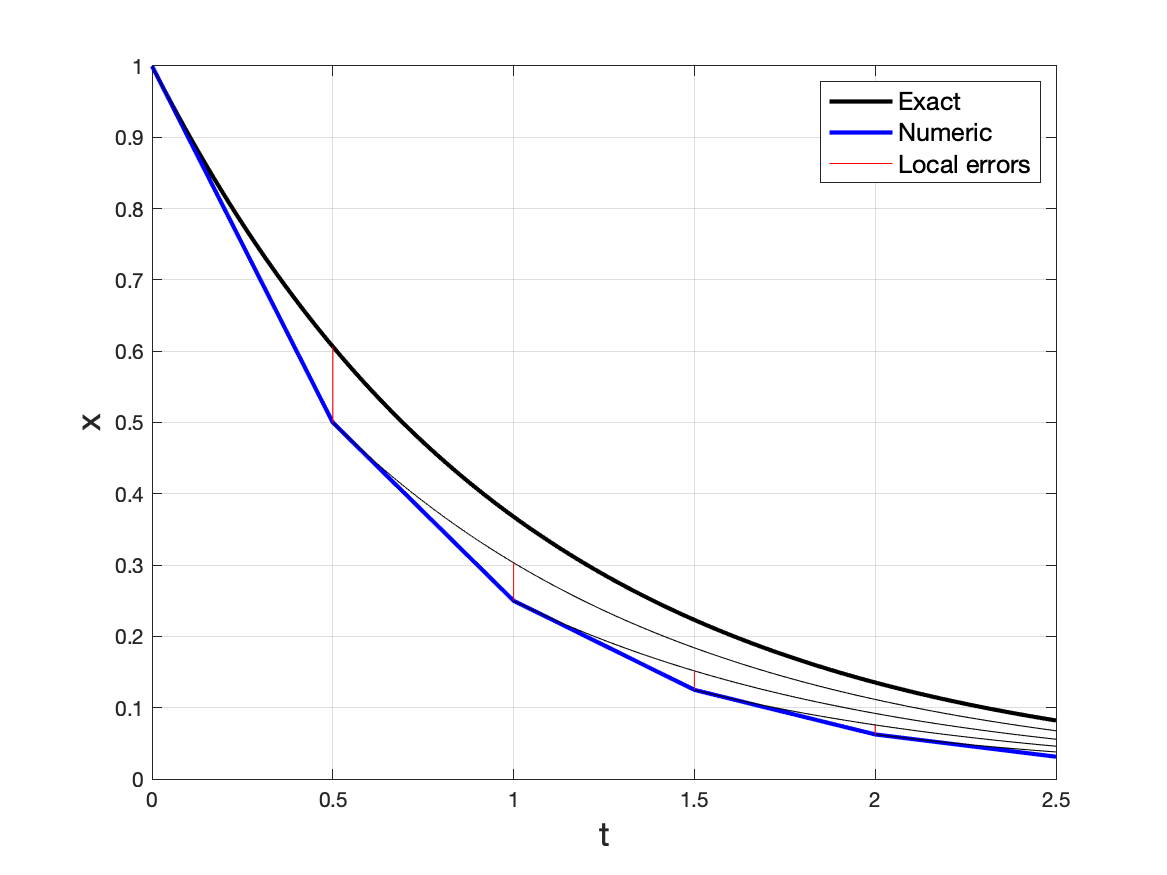
\includegraphics[width=10cm]{graphics/opg1/local_err0.png}
    \caption{Test equation with $\lambda=-1$ and $x_0=1$.}
    \label{fig1:local_err0}
\end{figure}


\section{Local and global truncation error on the test equation}
Obviously, both the local and global truncation errors depend on the method used---some methods will yield lower errors for the same step size, but might also be more demanding to compute. We will now compare a few different methods, namely 
\begin{itemize}
    \item[a)] the explicit Euler method (fixed step size),
    \item[b)] the implicit Euler method (fixed step size), and 
    \item[c)] the classical Runge-Kutta.
\end{itemize}
Specifically, we will use the methods in mention on the IVP from Equation \ref{eq:ivp1} with a fixed step size at $h=0.25$. Figure \ref{fig1:local_err1} shows the absolute value of the local truncation errors for the three methods. Notice that the errors are large initially but over time goes towards zero. This is because all three methods follow the behaviour of the exact solution to the test equation with these parameters---but more on that later. Also notice the difference between the explicit and implicit Euler methods and the classical Runge-Kutta (RK4). This difference is to do with the \textit{order} of the methods, which we will touch upon shortly.

\begin{figure}[H]
    \centering
    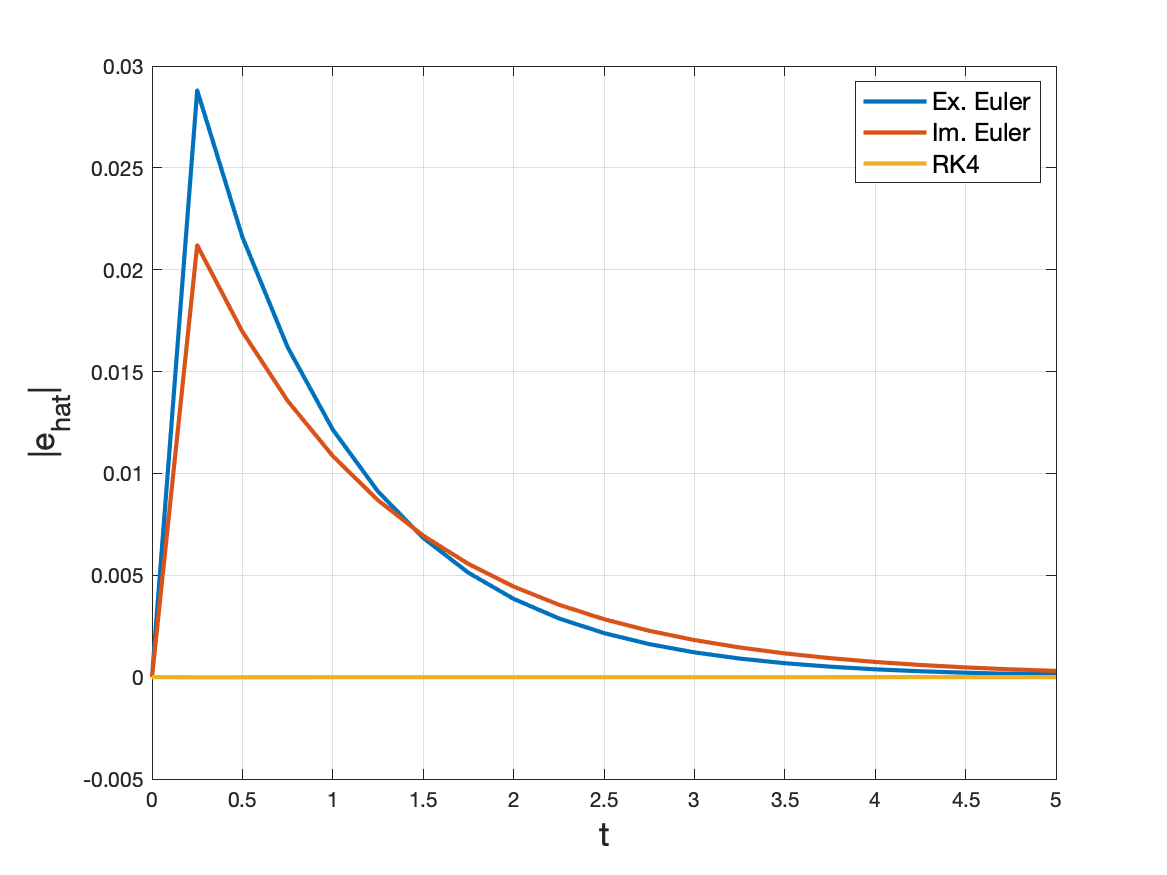
\includegraphics[width=10cm]{graphics/opg1/local_err1.png}
    \caption{Local truncation errors to test equation with $\lambda=-1$ and $x_0=1$ using different numerical methods.}
    \label{fig1:local_err1}
\end{figure}

Figure \ref{fig1:global_err1} shows the absolute value of the global truncation errors to the test equation with the given parameters for the three numerical methods in mention. Once again we see the behaviour where the errors are greatest initially and then decrease over time. This is again to do with the parameters in the test equation and the \textit{stability} of the methods used. Shortly, we will understand this better.

\begin{figure}[H]
    \centering
    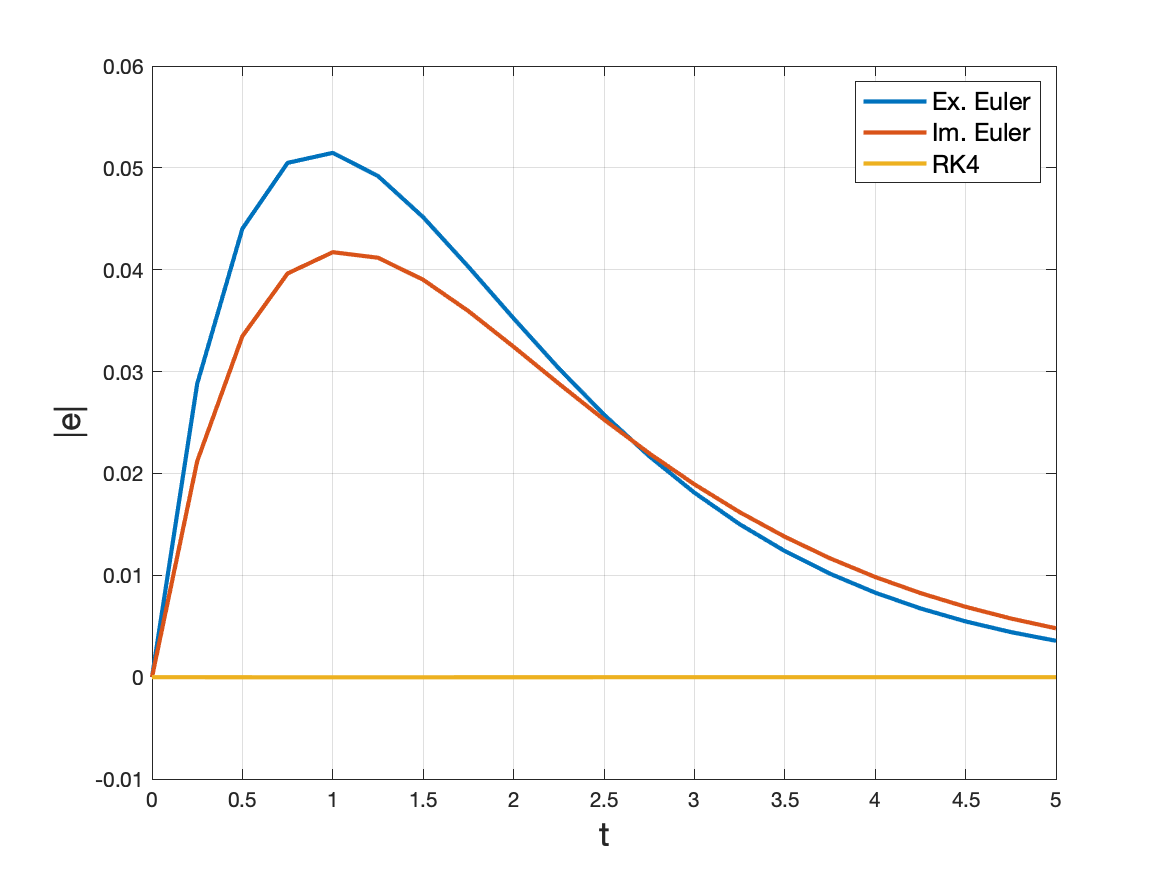
\includegraphics[width=10cm]{graphics/opg1/global_err1.png}
    \caption{Global truncation errors to test equation with $\lambda=-1$ and $x_0=1$ using different numerical methods.}
    \label{fig1:global_err1}
\end{figure}

\section{Local errors by step size}
The step size, $h$, plays an important role in the accuracy, i.e., the magnitude of local and/or global truncation errors, of any numerical method. Figure \ref{fig1:local_err2} shows the local error vs the time step for the numerical methods. Notice that the local truncation errors for both explicit and implicit Euler seem to roughly follow a linear trend. The local errors of the RK4 follow a higher order curve---from this plot alone it is difficult to determine the exact order.

\begin{figure}[H]
    \centering
    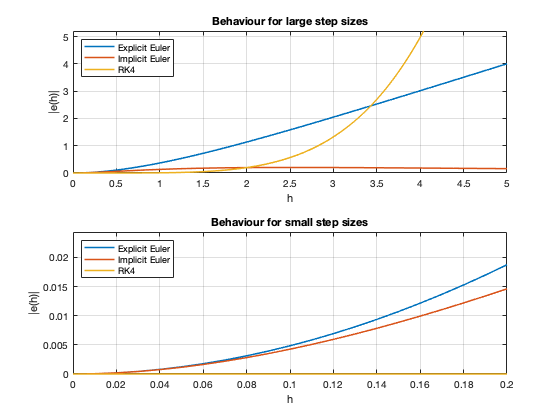
\includegraphics[width=10cm]{graphics/opg1/local_err_h.png}
    \caption{Local truncation errors as function of step size, $h$.}
    \label{fig1:local_err2}
\end{figure}

In fact, the local error has very much to do with the previously mentioned \textit{order} of the numerical method. Cf Ascher\cite{Ascher} a numerical method is said to have order $p$ if
\begin{align}
    e_t &= \mathcal{O}(h^p).
\end{align}
It turn out that the numerical methods in mention have order
\begin{align*}
    Explicit \ Euler:& \quad 1 \quad\quad\quad &&& \\
    Implicit \ Euler:& \quad 1 \quad\quad\quad &&& \\
    RK4:& \quad 4. \quad\quad\quad &&&
\end{align*}
The order of the methods will be shown later in this report.

\section{Global errors at t=1}
The order of the method has a large impact on the global truncation errors as just shown. However, the order also have a large impact on the global truncation errors. To demonstrate this, we re-use the IVP from Equation \ref{eq:ivp1}, at look at the global truncation error, i.e., the difference between the exact and the numerical solution, at $t=1$. We can do this for varying step sizes, $h$, and thereby get an idea of the impact. Figure \ref{fig1:err_t1} shows the absolute value of the global truncation errors at $t=1$, i.e., $|e_1|$. 

\begin{figure}[H]
    \centering
    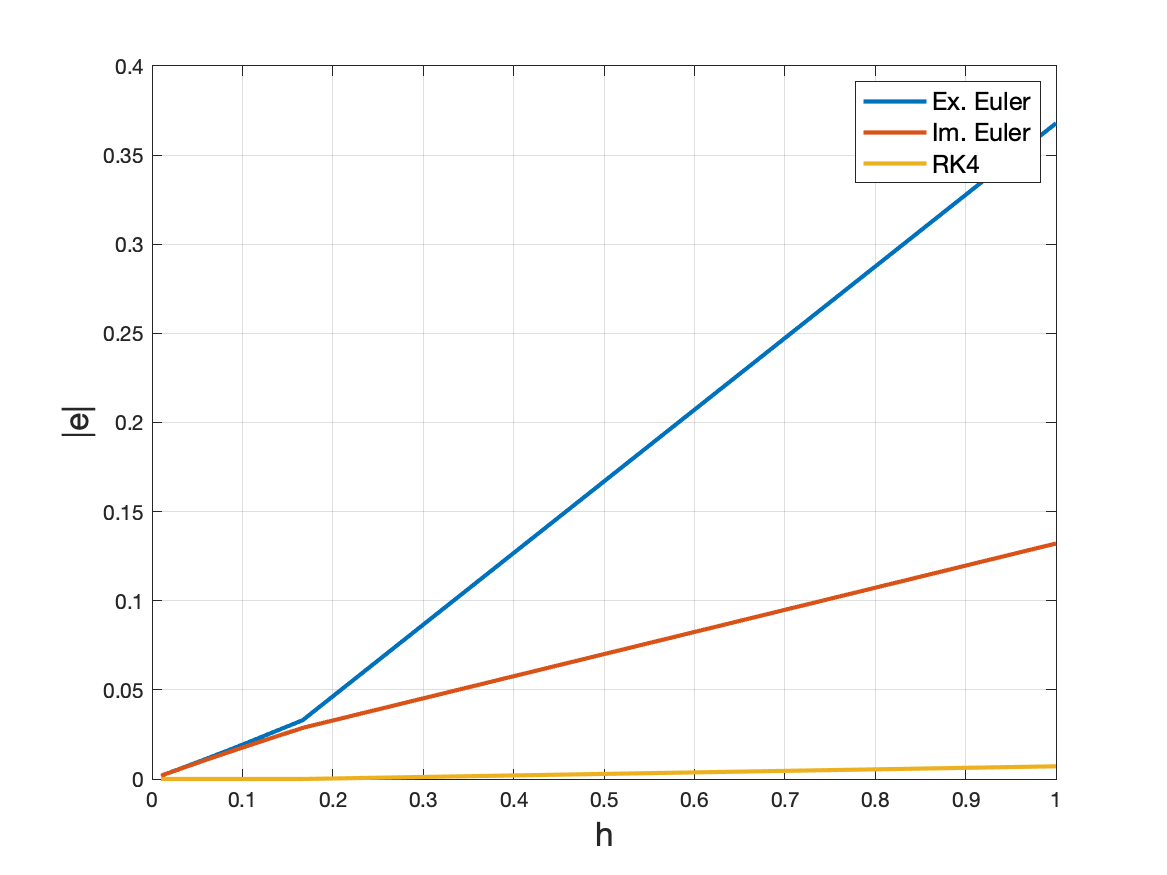
\includegraphics[width=10cm]{graphics/opg1/err_t1.png}
    \caption{Global truncation error to test equation with $\lambda=-1$ and $x_0=1$ using different numerical methods at $t=1$.}
    \label{fig1:err_t1}
\end{figure}

Notice that the absolute value of the global truncation errors of both the explicit and implicit Euler methods seem to increase linearly with the size of the time steps. This aligns with the order of the methods, since they are both methods of order 1. Since the classical Runge-Kutta method is of order 4, we would expect the global truncation error to follow $h^4$. However, based on this relatively small interval, it is difficult to see if that is actually the case. We can, however, see that the global truncation errors of RK4 are significantly lower than both the explicit and implicit Euler methods for the same time step sizes. 

\section{Stability of a numerical method}
As previously mentioned, \textit{stability}, i.e., how the methods converge, of numerical methods are an important characteristic of any numerical method. We have now introduced the test equation, and we will use this to say something about the stability of numerical methods. It is important to remember that stability is seen in this exact context, i.e., how the method perform on the test equation with a given set of parameters. 

Before we define exactly what we mean by stability of a numerical method, we need a little bit of framework. To investigate the properties of a numerical method, we write it on the form
\begin{align}
    x(t+h) &= R(\mu) x(t),
\end{align}
where the structure of $R(\cdot)$ depends on the numerical method used. 

A method is said to be \textit{stable} for some $\mu$ whenever $|R(\mu)| \leq 1$. Notice that \textit{stability} depends on the specific value for $\mu$. If we have that 
\begin{align}
    Re(\lambda) \leq 0 \quad \Leftrightarrow \quad |R(\mu)| \leq 1
\end{align}
we say that the method is \textit{A-stable}. Notice this means that for any $\lambda \leq 0$ we have stability, i.e., what we usually expect in the analytic case. 

If we further have that 
\begin{align}
    Re(\lambda) \rightarrow -\infty \quad \Rightarrow \quad |R(\mu)| \rightarrow 0
\end{align}
i.e., the method will converge in fewer steps when $\lambda$ becomes more negative, we say that the method is \textit{L-stable}. 

Let us look at a few examples. We will start with the explicit Euler method. The explicit Euler method is defined by 
\begin{align}
    x(t+h) &= x(t) + \lambda x(t) h \\
    &= (1+\lambda h) x(t).
\end{align}
So we have 
\begin{align}
    R(\mu) = 1 + \mu.
\end{align}
We can now define the stability region, $\mathcal{S}$, as the region where the method is stable. The stability region is therefore given by
\begin{align}
    \mathcal{S} = \left \{ \mu \in \mathcal{C} \ | \ |1+\mu| \leq 1 \right \}.
\end{align}

Figure \ref{fig1:ex_stability} shows stability region of the explicit Euler method. Notice that the method is only stable of a small circular region of $\mu=\lambda h$. Notice that this means that it is possible that the explicit Euler method does not converge, even if the exact solution does, i.e., the problem \textit{is} stable. It is therefore evident that the method is neither A nor L-stable.

\begin{figure}[H]
    \centering
    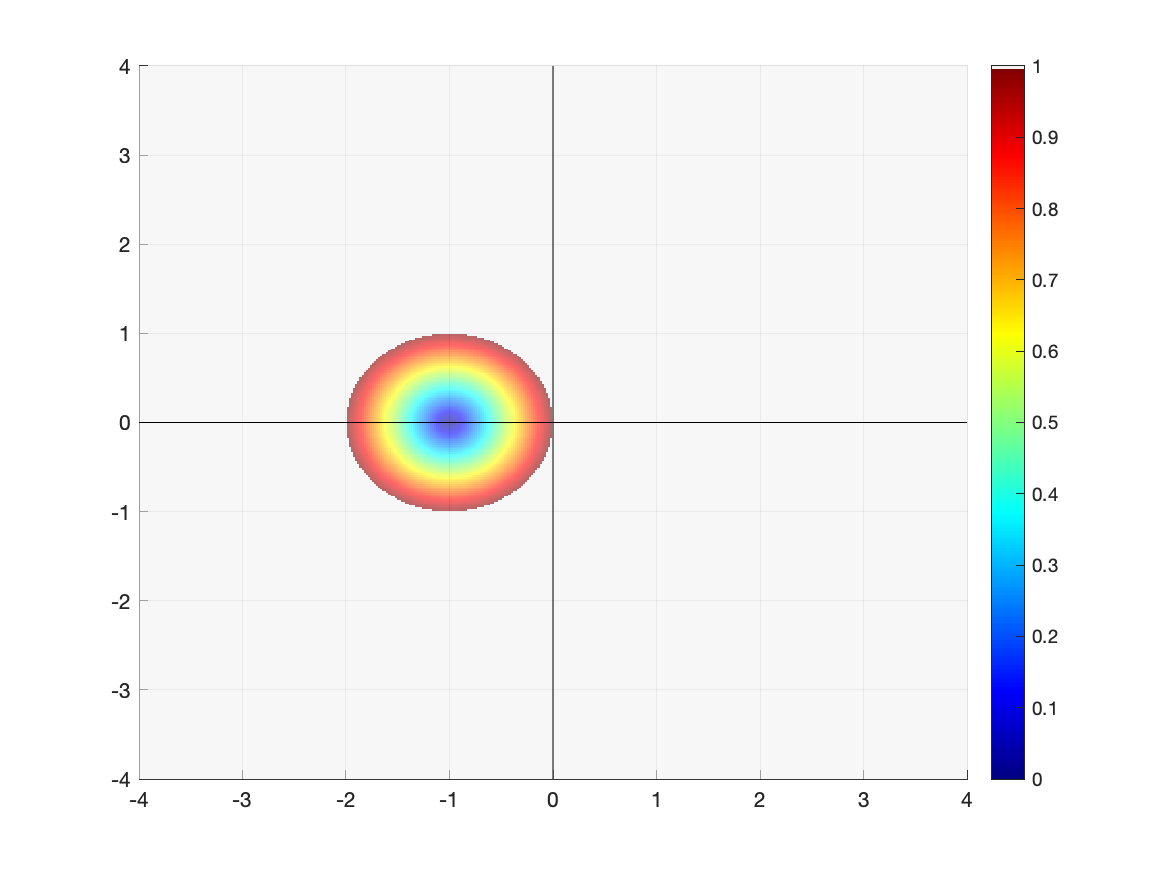
\includegraphics[width=10cm]{graphics/opg1/ex_stability.png}
    \caption{Stability region of the explicit Euler method on test equation. The colored region is the stable region.}
    \label{fig1:ex_stability}
\end{figure}


The implicit Euler method is given by
\begin{align}
    x(t+h) &= x(t) + \lambda x(t+h) h \\
    &= \frac{1}{1-\lambda h} x(t).
\end{align}
So we have 
\begin{align}
    R(\mu) = \frac{1}{1-\mu}.
\end{align}
We can now define the stability region, $\mathcal{S}$, for the implicit Euler method by
\begin{align}
    \mathcal{S} = \left \{ \mu \in \mathcal{C} \ | \ |\frac{1}{1-\mu}| \leq 1 \right \}.
\end{align}

Figure \ref{fig1:im_stability} shows the stability region of the implicit Euler method. Notice that a much larger area is stable than the for the explicit Euler method. In fact, the method is stable for all $Re(\lambda) \leq 0$, which tells us that the implicit Euler method is A-stable. Additionally, if we take a closer look at $R(\lambda h) = \frac{1}{1-\lambda h}$, we see that it goes towards $0$ for $\lambda \rightarrow -\infty$. Therefore the implicit Euler method is also L-stable. 

\begin{figure}[H]
    \centering
    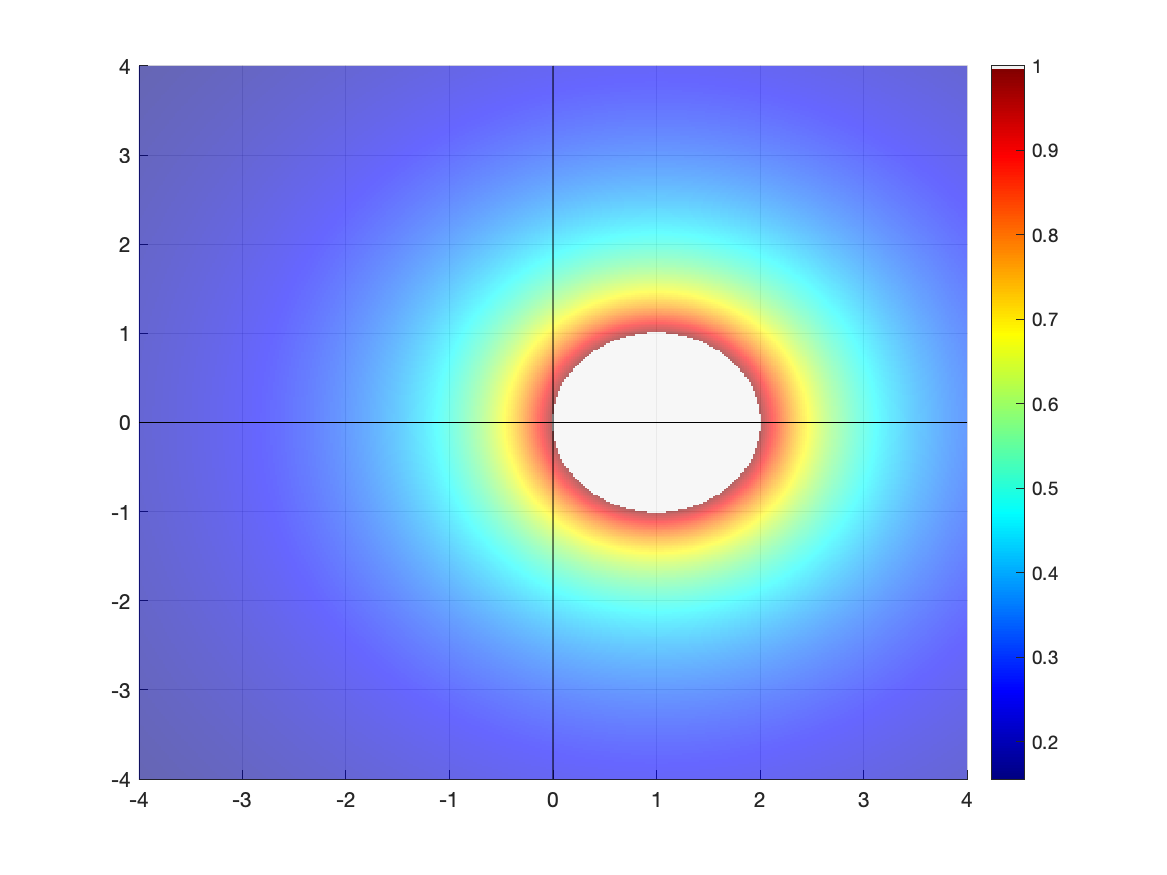
\includegraphics[width=10cm]{graphics/opg1/im_stability.png}
    \caption{Stability region of the implicit Euler method on test equation. The colored region is the stable region.}
    \label{fig1:im_stability}
\end{figure}

In fact, the implicit Euler method is \textit{too} stable. Notice that the method is stable even for some $Re(\lambda)>0$. This means that the implicit Euler method might converge even when the test equation is unstable! 

The classical Runge-Kutta method is a bit more complicated. We will therefore not derive the stability function, $R(\cdot)$ for RK4 here. Cf. Ascher\cite{Ascher}, the stability function for RK4 can be written as
\begin{align}
    R(\mu) = 1 + \mu + \frac{1}{2}\mu^2 + \frac{1}{6} \mu^3 + \frac{1}{24} \mu^4.
\end{align}
This gives us a region of stability, $\mathcal{S}$, as
\begin{align}
    \mathcal{S} = \left \{ \mu \in \mathcal{C} \ | \ | 1 + \mu + \frac{1}{2}\mu^2 + \frac{1}{6} \mu^3 + \frac{1}{24} \mu^4| \leq 1 \right \}.
\end{align}
Figure \ref{fig1:rk4_stability} shows the stability region for the classical Runge-Kutta method. Notice that the stability region is much like that of the explicit Euler method, in the sense that it is a small well defined region, albeit slightly larger. This also means that the classical Runge-Kutta method is neither A- nor L-stable. The real advantage of RK4 is not because is has a larger region of stability that the explicit Euler method, it is rather the fact that it is a 4th order method, and as such will be much more accurate. 

\begin{figure}[H]
    \centering
    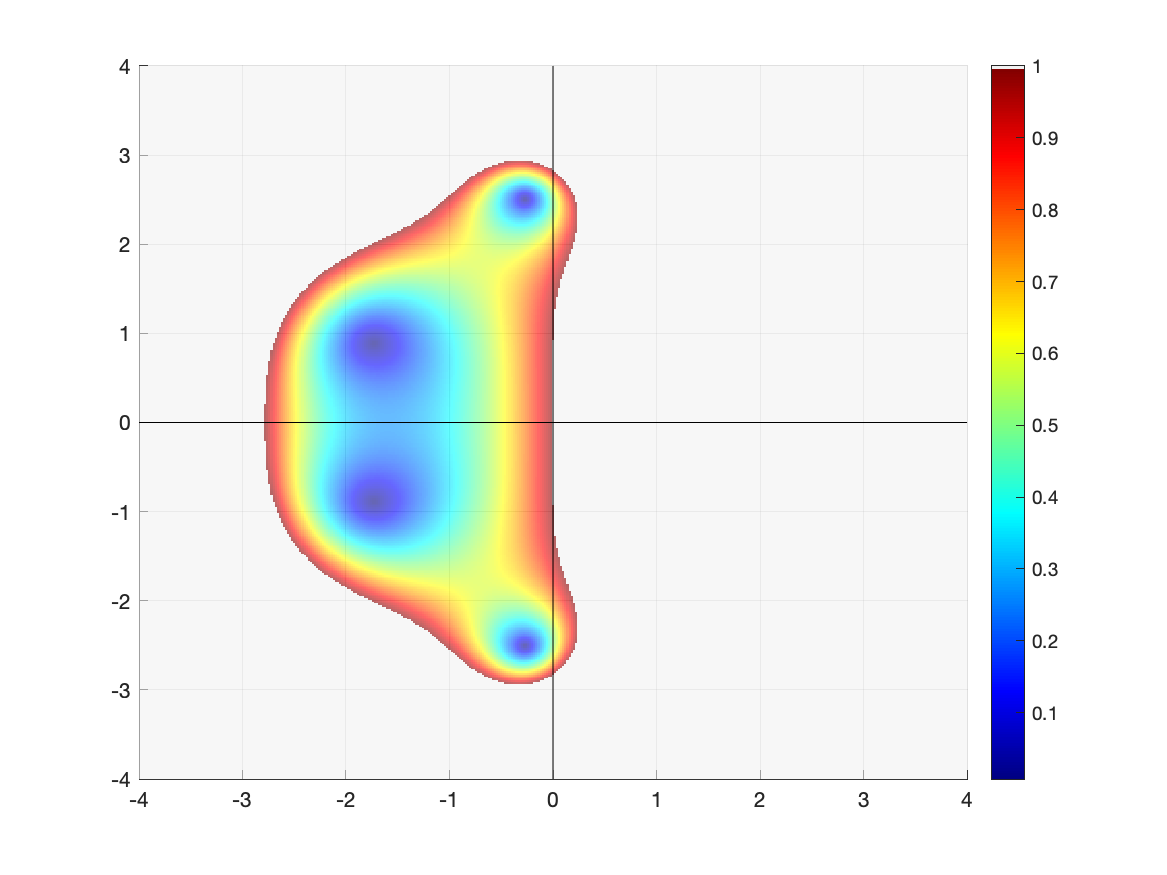
\includegraphics[width=10cm]{graphics/opg1/rk4_stability.png}
    \caption{Stability region of the classical Runge-Kutta method on test equation. The colored region is the stable region.}
    \label{fig1:rk4_stability}
\end{figure}










\clearforchapter
\chapter{Explicit ODE solver}
In the following, we consider the initial value problem (IVP) on the form
\begin{align}
    \dot{x}(t) &= f(t,x(t),p), & x(t_0) = x_0,
\end{align}
where $x \in \probR ^{n_x}$ and $p \in \probR ^{n_p}$. 

\section{Description of explicit Euler}
Our goal is to solve the IVP using a scientific, i.e., numeric, method. We remember that $\dot{x}(t)$ is given by the limit (multiple equal limits exist)
\begin{align}
    \dot{x}(t) &:= \lim_{h \rightarrow 0} \frac{x(t+h)-x(t)}{h}.
\end{align}
Since we are using numerical methods, we cannot represent the actual limit value. Instead, we have to use some finite approximation thereof. Choosing some $h>0$ therefore naturally leads to the approximation
\begin{align}
    \dot{x}(t) &\approx \frac{x(t+h)-x(t)}{h}, &h>0.
\end{align}
By rearranging the terms (isolating $x(t+h)$) we get
\begin{align}
    x(t+h) \approx x(t) + \dot{x}(t) h.
\end{align}
In fact, this corresponds to a first order Taylor expansion around $t$! From our basic course in calculus we therefore know that
\begin{align}
    x(t+h) &= x(t) + \dot{x}(t) h + \mathcal{O}(h^2).
    \label{eq2:ex_euler}
\end{align}
We now have a way to determine $x(t+h)$. This method is known as the explicit Euler method. 

\section{Explicit Euler fixed time step implementation}
When using the explicit Euler method, it is important to choose a suitable step size, $h$. Figure \ref{fig1:ex_stability} shows the stability region of the explicit Euler method for $\mu = \lambda h$ for the test equation. Notice that \textit{suitable} has to be seen in the in the context of the problem at hand. The most simple approach is to use a fixed step size; however, when doing so the user must select it very carefully. Listing \ref{lst2:ex_euler} shows an matlab implementation of the explicit Euler method.

\begin{lstlisting}[language=Matlab,caption=Explicit Euler with fixed step size,label=lst2:ex_euler]
function [t,x] = ExplicitEuler(fun,t0,tn,n,x0,varargin)
    % Explicit euler scheme 
    % f(x_t+1) = f(x_t) + f'(x_t)*h
    
    h = (tn-t0)/n; % Set the step size
    nx = size(x0,1);
    x = zeros(nx,n+1);
    t = zeros(1,n+1);

	t(:,1) = t0;
	x(:,1) = x0;
    for k=1:n
        f = feval(fun,t(k),x(:,k),varargin{:}); % make function evaluation 
        t(:,k+1) = t(:,k) + h;  % update the time step
        x(:,k+1) = x(:,k) + f*h; % update the function value
    end
	t = t';
	x = x';
\end{lstlisting}


\section{Explicit Euler adaptive time step implementation}
Sometimes it can be difficult to select a suitable step size, $h$. When dealing with problem with a more rich dynamic than the test equation, we might see that a smaller step size might be required in parts of the solution than others. To overcome this problem with a fixed step size, we must select a small step size and use that everywhere. However, this comes with a significant penalty to the speed, since we could get away with using a larger step size in most of the solution. This problem leads to a natural desire to construct an algorithm that can change the step size adaptively. The goal is to use as large step size as possible, while maintaining a sufficient accuracy in the individual steps. 

We therefore need some way of estimating the error, we do so using what is known as \textit{step doubling}. We have
\begin{align}
    x_{k+1} &= x_k + hf(t_k,x_k), \\
    \hat{x}_{k+1/2} &= x_k + \frac{h}{2}f(t_k,x_k), \ \text{and} \\
    \hat{x}_{k} &= \hat{x}_{k+1/2} + \frac{h}{2}f(t_k+\frac{h}{2},\hat{x}_{k+1/2}).
\end{align}
We now get the error estimate by means of step doubling by
\begin{align}
    e_{k+1} &= \hat{x}_{k+1} - x_{k+1}.
\end{align}
We are now able to define how to select the best step size, $h$. We do so by the \textit{asymptotic step size controller}, this means that our step size is given by
\begin{align}
    h_{k+1} &= \left(\frac{\varepsilon}{r_{k+1}} \right )^{1/2} h_k.
\end{align}
Where $r_{k+1}$ is found by
\begin{align}
    r_{k+1} &= \max_{i \in \{1,...,n_x\}} \left \{ \frac{|e_{k+1}|_i}{ \max \{ |\text{abstol}|_i, \ |x_{k+1}|_i \cdot |\text{reltol}|_i \} } \right \}
\end{align}
where $|\text{abstol}|_i$ and $|\text{reltol}|_i$ are the absolute and relative tolerance of $(x_{k+1})_i$ respectively. Listing \ref{lst2:ex_euler_adap} shows a matlab implementation of explicit Euler method with step doubling and asymptotic step size controller. 

\begin{lstlisting}[language=Matlab,caption=Explicit Euler with adaptive step size.,label=lst2:ex_euler_adap]
function [T,X,E,H,count_nfun,count_acp,count_rej] = ExplicitEulerAdaptiveStep(fun,tspan,x0,h0,abstol,reltol,varargin)
    % Explicit euler scheme with adaptive step length (h)
    % f(x_t+1) = f(x_t) + f'(x_t)*h
    
    epstol = 0.8; 
    facmin = 0.1; 
    facmax = 5.0; 

    t0 = tspan(1); 
    tf = tspan(2); 

    t = t0; 
    h = h0; 
    x = x0; 

    T = t; 
    X = x'; 
    E = 0;
    H = h0; 
    
    count_acp = 0; 
    count_step = 0; 
    count_nfun = 0; 
    count_rej = 0; 

    while t < tf 
        if (t+h>tf)
            h = tf - t; 
        end 

        f = feval(fun,t,x,varargin{:});
        AcceptStep = false;
        while ~AcceptStep
            x1 = x + h*f; 

            hm = 0.5*h; 
            tm = t + hm; 
            xm = x + hm*f; 
            fm = feval(fun,tm,xm,varargin{:});
            x1hat = xm + hm*fm; 

            e = x1hat-x1; 
            r = max( abs(e) ./ max(abstol, abs(x1hat).*reltol) ); 

            AcceptStep = (r <= 1.0);
            if AcceptStep
                t = t+h; 
                x = x1hat; 
                E = [E;abs(e)'];
                H = [H;h];

                T = [T;t];
                X = [X;x'];
                count_acp = count_acp + 1;
            else 
                count_rej = count_rej + 1; 
            end
            h = max(facmin, min(sqrt(epstol/r),facmax))*h; % change step size
            count_step = count_step + 1;
        end 
        count_nfun = count_step + count_rej;
    end
\end{lstlisting}


\section{Test on Van der Pol problem and comparison with Matlab ODE solvers}
Now that we have made an implementation of the explicit Euler method with both fixed and adaptive step size we want to compare these. To do so we look at the Van der Pol problem given by
\begin{align}
    \Ddot{x}(t) &= \mu (1-x(t)^2) \dot{x}(t) - x(t).
\end{align}
To solve the problem using the explicit Euler method we must first re-write the problem as a system of first order differential equations. Luckily this is done easily and given by
\begin{align}
    \dot{x}_1(t) &= x_2(t) \\
    \dot{x}_2(t) &= \mu(1-x_1(t)^2) x_2(t) - x_1(t).
\end{align}

We will now test the explicit Euler method on the Van der Pol problem with $\mu = 3$ and $\mu = 20$. 

\subsection{Van der Pol, $\mu = 3$}
The Van der Pol problem with $\mu = 3$ is a relatively straight forward non-stiff problem. There is no formal definition of when a problem is \textit{stiff}---only that whenever a problem change dynamics "very quickly" it is said to be. 

Figure \ref{fig2:fixed_mu3} shows the numerical solution to the Van der Pol problem with $\mu = 3$ for explicit Euler with $h \in \{0.1, 0.01, 0.001\}$, ODE45 and ODE15s. Notice that there is no visible difference between the solution obtained by ODE45 and ODE15s. Notice also that for $h=0.1$ there is a quite big difference between the explicit Euler solution and the other solutions; for $h=0.01$ the difference is smaller and for $h=0.001$ there is no visible difference anymore. This hints that it is a bad idea to use a step size larger than $h=0.001$ for this particular problem.

\begin{figure}[H]
    \centering
    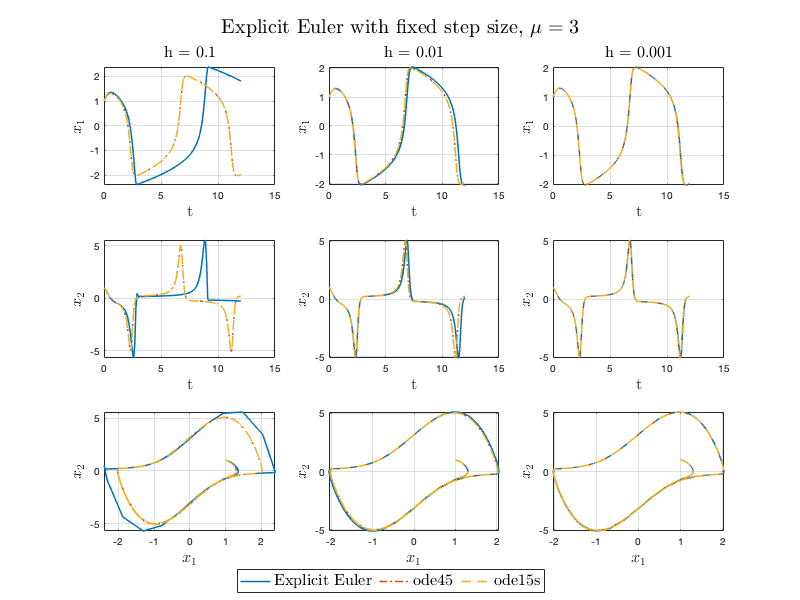
\includegraphics[width=\textwidth]{graphics/opg2/mu3_fixed.png}
    \caption{Solution to Van der Pol with $\mu = 3$ using fixed step sizes}
    \label{fig2:fixed_mu3}
\end{figure}

Table \ref{tab2:mu3_fixed} shows that CPU time and number of function evaluations when solving the Van der Pol problem with $\mu = 3$ using different time steps and Matlab ODE solvers. Notice that with $h=0.1$ the explicit Euler is much faster and uses less function evaluations that any of the other methods, however, as seen above the results are also quite poor. A time step of $h=0.01$ yields similar run time to ODE45---but with a slight deviation in the results. A step size of $h=0.001$ is by far the slowest of the methods, and the one that uses the most function evaluations. One of the reasons why ODE45 and ODE15s are able to outperform the explicit Euler with fixed step size is because they are able to adjust the step size such that a larger step size is used in the parts with a slower dynamic and vice versa. 

Notice that ODE45 seems to outperform ODE15s. This is a good indication that the problem is not particular stiff, i.e., it is not worth while to use an implicit method that comes with additional computational cost. 

\begin{table}[H]
    \centering
    \caption{CPU time and function evaluations of explicit Euler with fixed time step and Matlab ODE solvers}
    \begin{tabular}{|c||c|c|c|c|c|c|} \hline
         \textbf{Method}    & $h=0.1$&   $h=0.01$ & $h=0.001$ & ODE45 & ODE15s     \\ \hline \hline 
         \textbf{Time}      & 0.0007 &    0.0067  &    0.0389 & 0.0046 & 0.0175   \\ \hline
         \textbf{Fun evals} & 120   & 1200 & 12000 & 1069 & 926  \\ \hline
    \end{tabular}
    \label{tab2:mu3_fixed}
\end{table}



Figure \ref{fig2:adap_mu3} shows the numerical solution to the Van der Pol problem with $\mu = 3$ for explicit Euler with adaptive time steps and $AbsTol=RelTol \in \{10^{-2}, 10^{-4}, 10^{-6}\}$, ODE45 and ODE15s. Notice also that for $Tol = 10^{-2}$ there is a quite big difference between the explicit Euler solution and the other solutions; for $Tol = 10^{-4}$ the difference is almost not visible and for $Tol = 10^{-6}$ there is no visible difference anymore.

\begin{figure}[H]
    \centering
    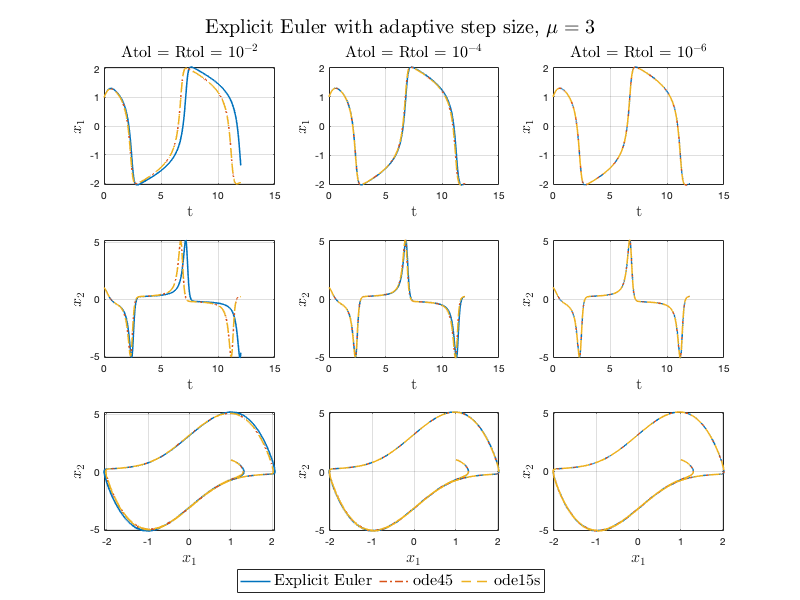
\includegraphics[width=\textwidth]{graphics/opg2/mu3_adap.png}
    \caption{Solution to Van der Pol with $\mu = 3$ using adaptive step sizes}
    \label{fig2:adap_mu3}
\end{figure}

Table \ref{tab2:mu3_adap} shows that CPU time and number of function evaluations when solving the Van der Pol problem with $\mu = 3$ using different tolerances and Matlab ODE solvers. Notice that with $Tol = 10^{-2}$ the explicit Euler is faster and uses less function evaluations that any of the other methods, however, as seen above the results are also quite poor. Using $Tol = 10^{-4}$ yields higher run time than ODE45, but with very little deviation in the results. Finally $Tol = 10^{-6}$ is by far the slowest of the methods, and the one that uses the most function evaluations. One of the reasons why ODE45 and ODE15s are able to outperform the explicit Euler with adaptive step size is because they are higher order method and implicit method respectively. This means that they are able to take larger step sizes, which requires less time.

\begin{table}[H]
    \centering
    \caption{CPU time and function evaluations of explicit Euler with adaptive time step and Matlab ODE solvers}
    \begin{tabular}{|c||c|c|c|c|c|c|} \hline
         \textbf{Method}    & $Tol = 10^{-2}$&   $Tol = 10^{-4}$ & $Tol = 10^{-6}$ & ODE45 & ODE15s     \\ \hline \hline 
         \textbf{Time}      & 0.0039  &  0.0730  &  0.1680 & 0.0046 & 0.0175   \\ \hline
         \textbf{Fun evals} & 482   & 4181 & 41780 & 1069 & 926  \\ \hline
    \end{tabular}
    \label{tab2:mu3_adap}
\end{table}

Figure \ref{fig2:adap_mu3_h} shows the used step sizes for the different tolerances. The red crosses mark whenever the step size controller failed to set the step size correctly, i.e., whenever the estimated (using step doubling) error was larger than the allowed maximum. Notice that the behaviour of all three tolerances are quite similar. Also notice that the step sizes vary by almost a factor 100! This means that even though the problem is not very stiff, there still is enough change in dynamics that the optimal step size vary by a factor 100. 

\begin{figure}[H]
    \centering
    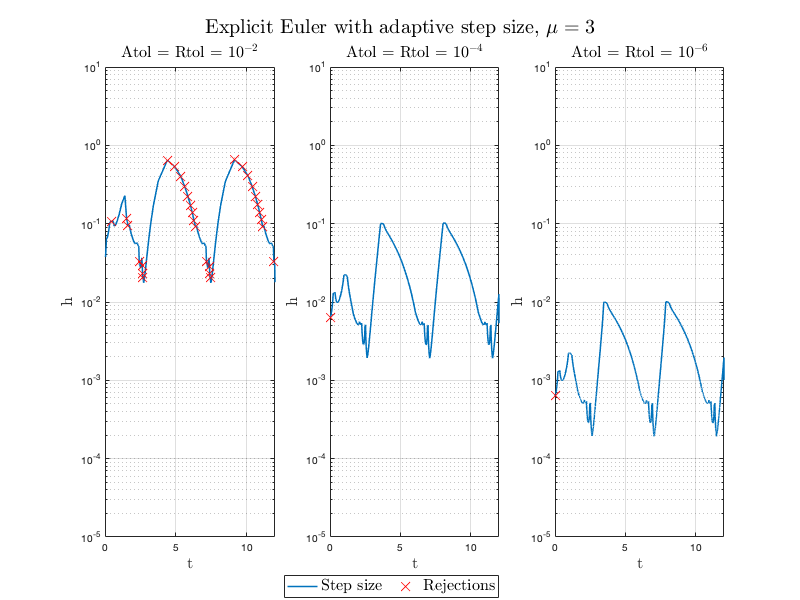
\includegraphics[width=\textwidth]{graphics/opg2/mu3_h.png}
    \caption{Step sizes when solving the Van der Pol with $\mu = 3$ at different tolerances}
    \label{fig2:adap_mu3_h}
\end{figure}

\subsection{Van der Pol, $\mu = 20$}
The Van der Pol problem with $\mu = 20$ is a more complicated problem. The dynamics of the problem is largely defined by the $\mu$ parameter. In particular, the problem becomes more stiff when $\mu$ is increased.

Figure \ref{fig2:fixed_mu20} shows the numerical solution to the Van der Pol problem with $\mu = 3$ for explicit Euler with $h \in \{0.1, 0.01, 0.001\}$, ODE45 and ODE15s. Notice that there is no visible difference between the solution obtained by ODE45 and ODE15s. For $h=0.1$ the solution diverges! It is not at all possible to solve the problem with such a large step size. There is a quite big difference between the explicit Euler solution and the other solutions for $h=0.01$. The difference is smaller for $h=0.001$, but it is still visible. This hints that it is a bad idea to use a step size larger than $h=0.001$ for this particular problem, and in fact we should use an even lower step size.

\begin{figure}[H]
    \centering
    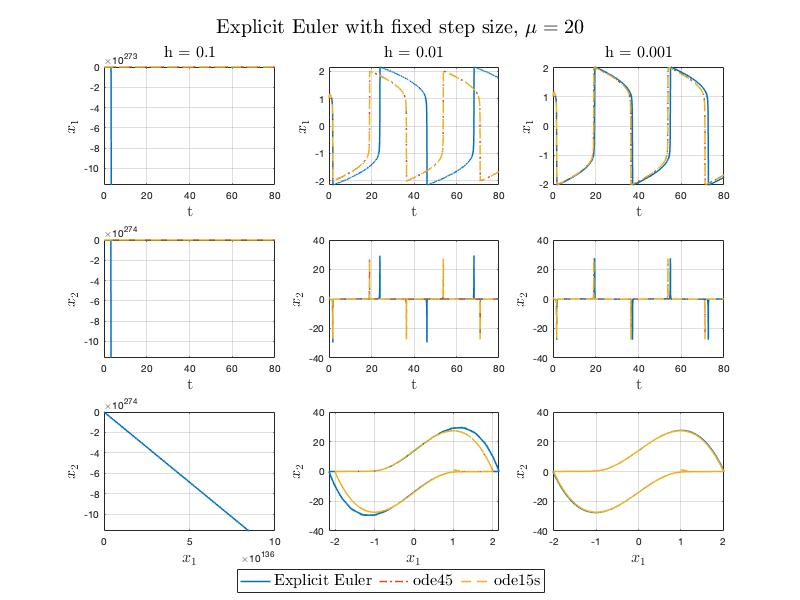
\includegraphics[width=\textwidth]{graphics/opg2/fixed_mu20.png}
    \caption{Solution to Van der Pol with $\mu = 20$ using fixed step sizes}
    \label{fig2:fixed_mu20}
\end{figure}

Table \ref{tab2:mu20_fixed} shows that CPU time and number of function evaluations when solving the Van der Pol problem with $\mu = 20$ using different time steps and Matlab ODE solvers. Notice that with $h=0.1$ the explicit Euler is much faster and uses less function evaluations that any of the other methods, however, as seen above the results are also completely wrong. A time step of $h=0.01$ yields similar run time to ODE45---but with substantial deviations in the results. A step size of $h=0.001$ is by far the slowest of the methods, and the one that uses the most function evaluations. One of the reasons why ODE45 and ODE15s are able to outperform the explicit Euler with fixed step size is because they are able to adjust the step size such that a larger step size is used in the parts with a slower dynamic and vice versa. 

Notice that ODE45 does not outperform ODE15s anymore. This is a good indication that the problem is stiff, i.e., it is worth while to use an implicit method that even when it comes with additional computational cost. The implicit method is also able to use far less function evaluations than the DoPri54. 

\begin{table}[H]
    \centering
    \caption{CPU time and function evaluations of explicit Euler with fixed time step and Matlab ODE solvers}
    \begin{tabular}{|c||c|c|c|c|c|c|} \hline
         \textbf{Method}    & $h=0.1$&   $h=0.01$ & $h=0.001$ & ODE45 & ODE15s     \\ \hline \hline 
         \textbf{Time}      & 0.0090  &  0.0382   &  0.2671 & 0.0370 & 0.0504   \\ \hline
         \textbf{Fun evals} & 800    &    8000    &   80000 & 8461 & 926  \\ \hline
    \end{tabular}
    \label{tab2:mu20_fixed}
\end{table}



Figure \ref{fig2:adap_mu20} shows the numerical solution to the Van der Pol problem with $\mu = 20$ for explicit Euler with adaptive time steps and $AbsTol=RelTol \in \{10^{-2}, 10^{-4}, 10^{-6}\}$, ODE45 and ODE15s. Notice also that for $Tol = 10^{-2}$ there is a quite big difference between the explicit Euler solution and the other solutions; for $Tol = 10^{-4}$ the difference is almost not visible and for $Tol = 10^{-6}$ there is no visible difference anymore.

\begin{figure}[H]
    \centering
    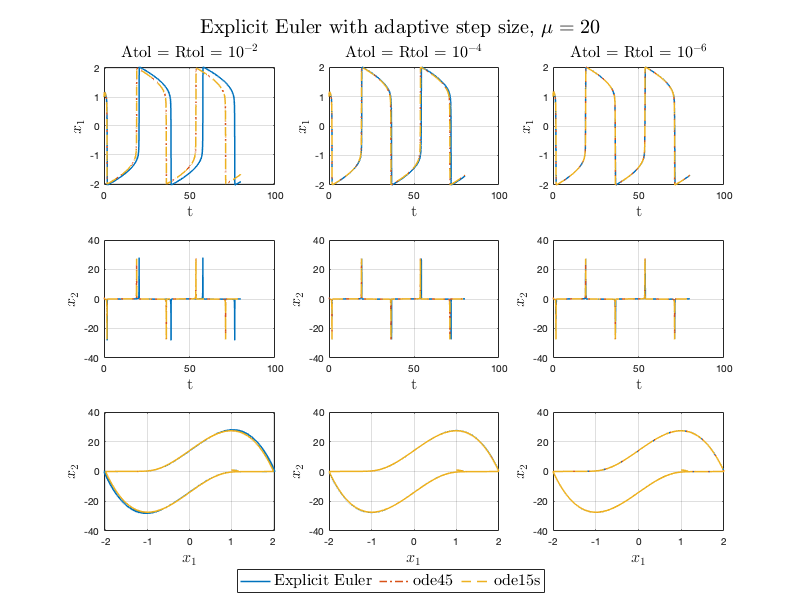
\includegraphics[width=\textwidth]{graphics/opg2/mu20_adap.png}
    \caption{Solution to Van der Pol with $\mu = 20$ using adaptive step sizes}
    \label{fig2:adap_mu20}
\end{figure}

Table \ref{tab2:mu20_adap} shows the CPU time and number of function evaluations when solving the Van der Pol problem with $\mu = 20$ using different tolerances and Matlab ODE solvers. Notice that with $Tol = 10^{-2}$ the explicit Euler is faster and uses less function evaluations that any of the other methods (as many as ODE15s), however, as seen above the results also deviate from the rest. Using $Tol = 10^{-4}$ yields higher run time than ODE45 and ODE15s, but with very little deviation in the results. Finally $Tol = 10^{-6}$ is by far the slowest of the methods, and the one that uses the most function evaluations (by a quite substantial amount). One of the reasons why ODE45 and ODE15s are able to outperform the explicit Euler with adaptive step size is because they are higher order method and implicit method respectively. This means that they are able to take larger step sizes, which requires less time.

\begin{table}[H]
    \centering
    \caption{CPU time and function evaluations of explicit Euler with adaptive time step and Matlab ODE solvers}
    \begin{tabular}{|c||c|c|c|c|c|c|} \hline
         \textbf{Method}    & $Tol = 10^{-2}$&   $Tol = 10^{-4}$ & $Tol = 10^{-6}$ & ODE45 & ODE15s     \\ \hline \hline 
         \textbf{Time}      & 0.0131  &  0.2286  &  0.5656 & 0.0386 & 0.0612   \\ \hline
         \textbf{Fun evals} & 3137   &    13154  &    111656 & 8461 & 2944  \\ \hline
    \end{tabular}
    \label{tab2:mu20_adap}
\end{table}

Figure \ref{fig2:adap_mu20_h} shows the used step sizes for the different tolerances. The red crosses mark whenever the step size controller failed to set the step size correctly, i.e., whenever the estimated (using step doubling) error was larger than the allowed maximum. Notice that the behaviour of all three tolerances are quite similar. Also notice that the step sizes vary by more than a factor 1000! This is a good indication that the problem is stiff. Also notice that for $AbsTol=RelTol \in \{10^{-2}, 10^{-4}\}$ the step size controller fails at setting the correct step size many times. This again indicates that there is a rapid change in dynamics, which leads to a large needed change in step size.

\begin{figure}[H]
    \centering
    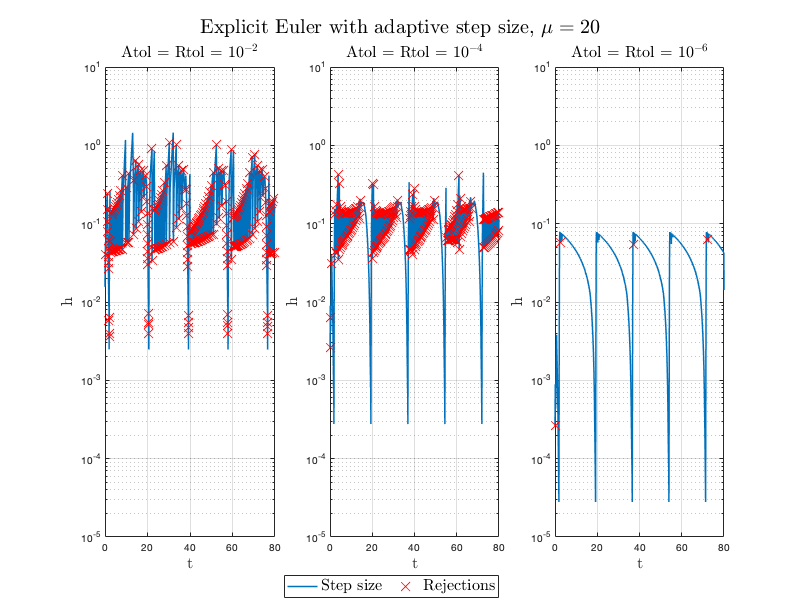
\includegraphics[width=\textwidth]{graphics/opg2/mu20_h.png}
    \caption{Step sizes when solving the Van der Pol with $\mu = 20$ at different tolerances}
    \label{fig2:adap_mu20_h}
\end{figure}






\clearforchapter
\chapter{Implicit ODE solver}
In the following, we consider the initial value problem (IVP) on the form
\begin{align}
    \dot{x}(t) &= f(t,x(t),p), & x(t_0) = x_0,
\end{align}
where $x \in \probR ^{n_x}$ and $p \in \probR ^{n_p}$. 

\section{Description of implicit Euler}
Our goal is to solve the IVP using a scientific, i.e., numeric, method. We note that $\dot{x}(t+h)$ is given by the limit (multiple equal limits exist)
\begin{align}
    \lim_{h \rightarrow 0} \dot{x}(t+h) &:= \lim_{h \rightarrow 0} \frac{x(t+h)-x(t)}{h}.
\end{align}
Since we are using numerical methods, we cannot represent the actual limit value. Instead, we have to use some finite approximation thereof. Choosing some $h>0$ therefore naturally leads to the approximation
\begin{align}
    \dot{x}(t+h) &\approx \frac{x(t+h)-x(t)}{h}, &h>0.
\end{align}
By rearranging the terms (isolating $x(t+h)$) we get
\begin{align}
    x(t+h) \approx x(t+h) + \dot{x}(t) h.
\end{align}
In fact, this corresponds to a first order Taylor expansion. From our basic course in calculus we therefore know that
\begin{align}
    x(t+h) &= x(t) + \dot{x}(t+h) h + \mathcal{O}(h^2).
    \label{eq3:im_euler}
\end{align}
This method is known as the implicit Euler method. Notice that unlike the explicit Euler method we do not know all terms on the right hand side. In stead, we must solve the equation
\begin{align}
    x(t+h) - (x(t) + \dot{x}(t+h) h) &= 0.
\end{align}
This is usually done using e.g. Newton's method. However, since it is only an approximation, we might as well loosen the restriction a bit, and consider 
\begin{align}
    x(t+h) - (x(t) + \dot{x}(t+h) h) &\leq \varepsilon, & \varepsilon>0.
\end{align}
This is known as \textit{in-exact Newton} and might produce a significant increase in speed for the method. 

We now have an alternative way of estimating $x(t+h)$. The implicit Euler method is more stable for stiff problems, i.e., problems with rapidly changing dynamics. Since an equation must be solved for each step, the steps are generally more expensive than for the explicit Euler method, so the implicit method must only be used when needed. If we compare the stability regions of the test equation for the explicit and implicit methods, we see that the implicit Euler method has a much larger stability region than the explicit Euler method. So much so that the implicit Euler method might converge even when the problem is actually not stable! 

\section{Implicit Euler fixed time step implementation}
When using the implicit Euler method, it is important to choose a suitable step size, $h$. Figure \ref{fig1:im_stability} shows the stability region of the implicit Euler method for $\mu = \lambda h$ for the test equation. Notice that \textit{suitable} has to be seen in the in the context of the problem at hand. The most simple approach is to use a fixed step size; however, when doing so the user must select it very carefully. Listing \ref{lst3:im_euler} shows a Matlab implementation of the implicit Euler method.

\begin{lstlisting}[language=Matlab,caption=Implicit Euler with fixed step size.,label=lst3:im_euler]
function [t,x,count_f] = ImplicitEuler(fun,ta,tb,n,xa,varargin)
    % Implicit euler scheme
    % f(x_t+1) = f(x_t) + f'(x_t+1)*h
    
    h = (tb-ta)/n;
    nx = size(xa,1);
    x = zeros(nx,n+1);
    t = zeros(1,n+1);
    count_f = 0; 

    tol = 1.0e-6;
    maxit = 100;

    t(:,1) = ta;
    x(:,1) = xa;
    for k=1:n
        [f,~] = feval(fun,t(k),x(:,k),varargin{:});
        t(:,k+1) = t(:,k) + h;
        x0 = x(:,k) + h*f;
        [x(:,k+1),count,~] = NewtonsMethodODE(fun,t(:,k), x(:,k), h, x0, tol, maxit,varargin{:});
        count_f = count_f + count;
    end

    t = t';
    x = x';

    end
\end{lstlisting}

\section{Implicit Euler adaptive time step implementation}
Sometimes it can be difficult to select a suitable step size, $h$. When dealing with problem with a more rich dynamic than the test equation, we might see that a smaller step size might be required in parts of the solution than others. To overcome this problem with a fixed step size, we must select a small step size and use that everywhere. However, this comes with a significant penalty to the speed, since we could get away with using a larger step size in most of the solution. This problem leads to a natural desire to construct an algorithm that can change the step size adaptively. The goal is to use as large step size as possible, while maintaining a sufficient accuracy in the individual steps. 

We therefore need some way of estimating the error, we do so using what is known as \textit{step doubling}. We have
\begin{align}
    x_{k+1} &= x_k + hf(t_k,x_k), \\
    \hat{x}_{k+1/2} &= x_k + \frac{h}{2}f(t_k,x_k), \ \text{and} \\
    \hat{x}_{k} &= \hat{x}_{k+1/2} + \frac{h}{2}f(t_k+\frac{h}{2},\hat{x}_{k+1/2}).
\end{align}
We now get the error estimate by means of step doubling by
\begin{align}
    e_{k+1} &= \hat{x}_{k+1} - x_{k+1}.
\end{align}
We are now able to define how to select the best step size, $h$. We do so by the \textit{asymptotic step size controller}, this means that our step size is given by
\begin{align}
    h_{k+1} &= \left(\frac{\varepsilon}{r_{k+1}} \right )^{1/2} h_k.
\end{align}
Where $r_{k+1}$ is found by
\begin{align}
    r_{k+1} &= \max_{i \in \{1,...,n_x\}} \left \{ \frac{|e_{k+1}|_i}{ \max \{ |\text{abstol}|_i, \ |x_{k+1}|_i \cdot |\text{reltol}|_i \} } \right \}
\end{align}
where $|\text{abstol}|_i$ and $|\text{reltol}|_i$ are the absolute and relative tolerance of $(x_{k+1})_i$ respectively. Listing \ref{lst3:im_euler_adap} shows a matlab implementation of implicit Euler method with step doubling and asymptotic step size controller. 

\begin{lstlisting}[language=Matlab,caption=Implicit Euler with adaptive step size.,label=lst3:im_euler_adap]
function [T,X,E,R,H,count_nfun,count_acp,count_rej] = ImplicitEulerAdaptiveStep(fun,tspan,x0,h0,abstol,reltol,varargin)
    % Implicit euler scheme with adaptive step length (h)
    % f(x_t+1) = f(x_t) + f'(x_t+1)*h
    
    epstol = 0.8; 
    facmin = 0.1; 
    facmax = 5.0; 

    t0 = tspan(1); 
    tf = tspan(2); 

    t = t0; 
    h = h0; 
    x = x0; 

    T = t; 
    X = x'; 
    E = 0;
    R = 0;
    H = h0; 
    
    count_acp = 0; 
    count_step = 0; 
    count_nfun = 0; 
    count_rej = 0; 

    while t < tf 
        if (t+h>tf)
            h = tf - t; 
        end 

        f = feval(fun,t,x,varargin{:});
        AcceptStep = false;
        while ~AcceptStep
            x0 = x + h*f; 
            [x1,count1,~] = NewtonsMethodODE(fun,t, x, h, x0, tol, maxit,varargin{:});

            hm = 0.5*h; 
            tm = t + hm; 
            x0 = x + hm*f; 
            [xm,count2,~] = NewtonsMethodODE(fun,t, x, hm, x0, tol, maxit,varargin{:});

            fm = feval(fun,tm,xm,varargin{:});
            x0 = xm + hm*fm; 
            [x1hat,count3,~] = NewtonsMethodODE(fun,tm, xm, hm, x0, tol, maxit,varargin{:});

            e = x1hat-x1; 
            r = max( abs(e) ./ max(abstol, abs(x1hat).*reltol) ); 

            AcceptStep = (r <= 1.0);
            if AcceptStep
                t = t+h; 
                x = x1hat; 
                E = [E;abs(e)'];
                R = [R;r];
                H = [H;h];

                T = [T;t];
                X = [X;x'];
                count_acp = count_acp + 1;
            else 
                count_rej = count_rej + 1; 
            end
            h = max(facmin, min(sqrt(epstol/r),facmax))*h; % change step size
            count_step = count_step + 1;
            count_nfun = count_nfun + count1 + count2 + count3;
        end 
        count_nfun = count_nfun + count_step + count_rej;
    end 
\end{lstlisting}

\section{Test on Van der Pol problem and comparison with Matlab ODE solvers}
Now that we have made an implementation of the implicit Euler method with both fixed and adaptive step size we want to compare these. To do so we look at the Van der Pol problem given by
\begin{align}
    \Ddot{x}(t) &= \mu (1-x(t)^2) \dot{x}(t) - x(t).
\end{align}
To solve the problem using the implicit Euler method we must first re-write the problem as a system of first order differential equations. Luckily this is done easily and given by
\begin{align}
    \dot{x}_1(t) &= x_2(t) \\
    \dot{x}_2(t) &= \mu(1-x_1(t)^2) x_2(t) - x_1(t).
\end{align}

We will now test the implicit Euler method on the Van der Pol problem with $\mu = 3$ and $\mu = 20$. 

\subsection{Van der Pol, $\mu = 3$}
The Van der Pol problem with $\mu = 3$ is a relatively straight forward non-stiff problem. There is no formal definition of when a problem is \textit{stiff}---only that whenever a problem change dynamics "very quickly" it is said to be. 

Figure \ref{fig3:fixed_mu3} shows the numerical solution to the Van der Pol problem with $\mu = 3$ for implicit Euler with $h \in \{0.1, 0.01, 0.001\}$, ODE45 and ODE15s. Notice that there is no visible difference between the solution obtained by ODE45 and ODE15s. Notice also that for $h=0.1$ there is a quite big difference between the implicit Euler solution and the other solutions; for $h=0.01$ the difference is smaller and for $h=0.001$ there is no visible difference anymore. This hints that it is a bad idea to use a step size larger than $h=0.001$ for this particular problem.

\begin{figure}[H]
    \centering
    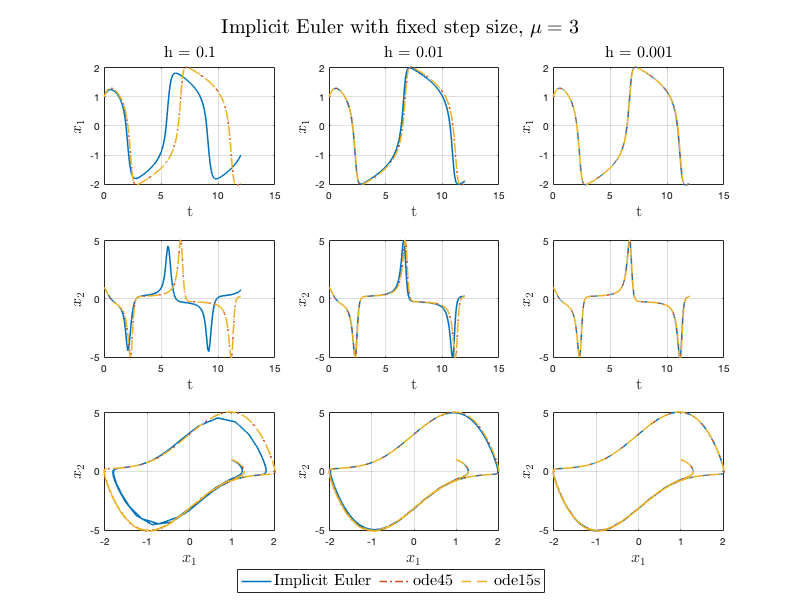
\includegraphics[width=\textwidth]{graphics/opg3/mu3_fixed.png}
    \caption{Solution to Van der Pol with $\mu = 3$ using fixed step sizes}
    \label{fig3:fixed_mu3}
\end{figure}

Table \ref{tab3:mu3_fixed} shows the CPU time and number of function evaluations when solving the Van der Pol problem with $\mu = 3$ using different time steps and Matlab ODE solvers. Notice that with $h=0.1$ the implicit Euler is much faster and uses less function evaluations that any of the other methods, however, as seen above the results are also quite poor. A time step of $h=0.01$ yields similar run time to ODE15s---but with a slight deviation in the results. A step size of $h=0.001$ is by far the slowest of the methods, and the one that uses the most function evaluations. One of the reasons why ODE45 and ODE15s are able to outperform the implicit Euler with fixed step size is because they are able to adjust the step size such that a larger step size is used in the parts with a slower dynamic and vice versa. 

Notice that ODE45 seems to outperform ODE15s. This is a good indication that the problem is not particular stiff, i.e., it is not worth while to use an implicit method that comes with additional computational cost. 

\begin{table}[H]
    \centering
    \caption{CPU time and function evaluations of implicit Euler with fixed time step and Matlab ODE solvers}
    \begin{tabular}{|c||c|c|c|c|c|c|} \hline
         \textbf{Method}    & $h=0.1$&   $h=0.01$ & $h=0.001$ & ODE45 & ODE15s     \\ \hline \hline 
         \textbf{Time}      & 0.0061 &   0.0162  &   0.0962 & 0.0046 & 0.0175   \\ \hline
         \textbf{Fun evals} & 807   &     5421   & 48001 & 1069 & 926  \\ \hline
    \end{tabular}
    \label{tab3:mu3_fixed}
\end{table}



Figure \ref{fig3:adap_mu3} shows the numerical solution to the Van der Pol problem with $\mu = 3$ for implicit Euler with adaptive time steps and $AbsTol=RelTol \in \{10^{-2}, 10^{-4}, 10^{-6}\}$, ODE45 and ODE15s. Notice also that for $Tol = 10^{-2}$ there is a quite big difference between the implicit Euler solution and the other solutions; for $Tol = 10^{-4}$ the difference is almost not visible and for $Tol = 10^{-6}$ there is no visible difference anymore.

\begin{figure}[H]
    \centering
    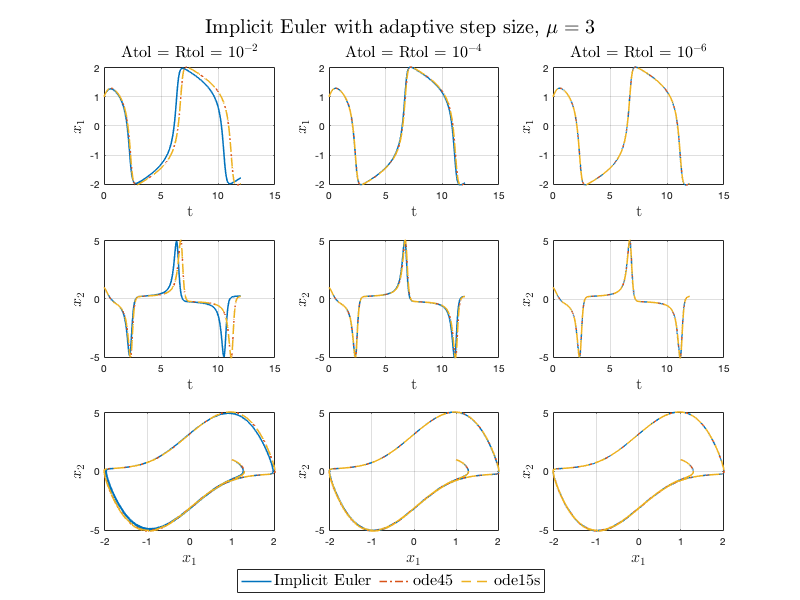
\includegraphics[width=\textwidth]{graphics/opg3/mu3_adap.png}
    \caption{Solution to Van der Pol with $\mu = 3$ using adaptive step sizes}
    \label{fig3:adap_mu3}
\end{figure}

Table \ref{tab3:mu3_adap} shows that CPU time and number of function evaluations when solving the Van der Pol problem with $\mu = 3$ using different tolerances and Matlab ODE solvers. Notice that with $Tol = 10^{-2}$ the implicit Euler is relatively fast (slower than ODE45 but faster than ODE15s), however, as seen above the results are also quite poor. Using $Tol = 10^{-4}$ yields higher run time than ODE15s, but with very little deviation in the results. Finally $Tol = 10^{-6}$ is by far the slowest of the methods, and the one that uses the most function evaluations. One of the reasons why ODE45 and ODE15s are able to outperform the implicit Euler with adaptive step size is because they are higher order methods. This means that they are able to take larger step sizes, which requires less time.

\begin{table}[H]
    \centering
    \caption{CPU time and function evaluations of implicit Euler with adaptive time step and Matlab ODE solvers}
    \begin{tabular}{|c||c|c|c|c|c|c|} \hline
         \textbf{Method}    & $Tol = 10^{-2}$&   $Tol = 10^{-4}$ & $Tol = 10^{-6}$ & ODE45 & ODE15s     \\ \hline \hline 
         \textbf{Time}      & 0.0127  &  0.0845  &  0.4249 & 0.0046 & 0.0175   \\ \hline
         \textbf{Fun evals} & 3575   &     16851    &   166983 & 1069 & 926  \\ \hline
    \end{tabular}
    \label{tab3:mu3_adap}
\end{table}

Figure \ref{fig3:adap_mu3_h} shows the used step sizes for the different tolerances. The red crosses mark whenever the step size controller failed to set the step size correctly, i.e., whenever the estimated (using step doubling) error was larger than the allowed maximum. Notice that the behaviour of all three tolerances are quite similar. Also notice that the step sizes vary by almost a factor 100! This means that even though the problem is not very stiff, there still is enough change in dynamics that the optimal step size vary by a factor 100. 

\begin{figure}[H]
    \centering
    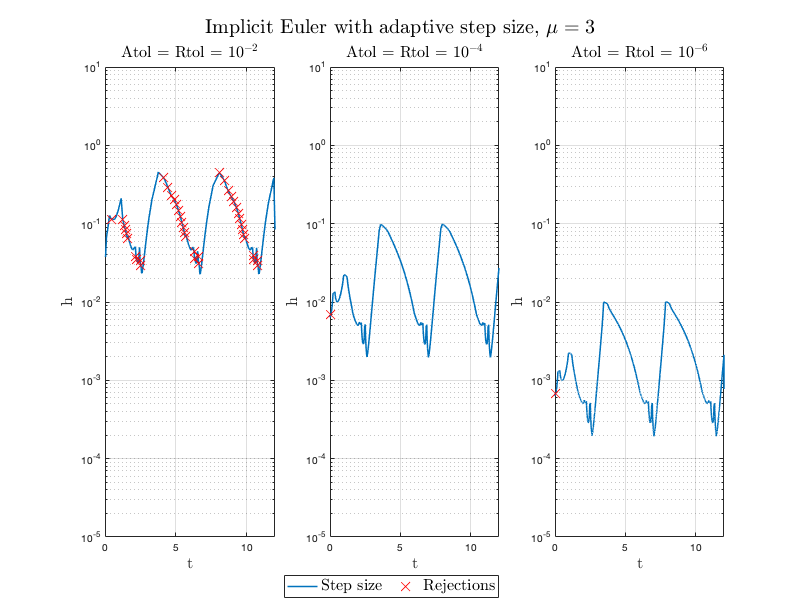
\includegraphics[width=\textwidth]{graphics/opg3/mu3_h.png}
    \caption{Step sizes when solving the Van der Pol with $\mu = 3$ at different tolerances}
    \label{fig3:adap_mu3_h}
\end{figure}

\subsection{Van der Pol, $\mu = 20$}
The Van der Pol problem with $\mu = 20$ is a more complicated problem. The dynamics of the problem is largely defined by the $\mu$ parameter. In particular, the problem becomes more stiff when $\mu$ is increased.

Figure \ref{fig3:fixed_mu20} shows the numerical solution to the Van der Pol problem with $\mu = 3$ for implicit Euler with $h \in \{0.1, 0.01, 0.001\}$, ODE45 and ODE15s. Notice that there is no visible difference between the solution obtained by ODE45 and ODE15s. For $h=0.1$ the solution does not diverge (as the explicit Euler did), however, it deviate substantially from the other solutions! There is a quite big difference between the implicit Euler solution and the other solutions for $h=0.01$. The difference is smaller for $h=0.001$, but it is still visible. This hints that it is a bad idea to use a step size larger than $h=0.001$ for this particular problem, and in fact we should use an even lower step size.

Notice that for the explicit Euler, we saw that the errors came because the curve was "behind" the rest, i.e., the sudden change in value for $x_1$ or $x_2$ came too late. Now we see the exact opposite---the sudden spikes comes too early. This is a key difference between the left point and right point method, i.e., explicit- and implicit Euler. The implicit Euler has much better convergence properties, which is also why we do not see any of the solutions diverge, albeit with some large errors. 

\begin{figure}[H]
    \centering
    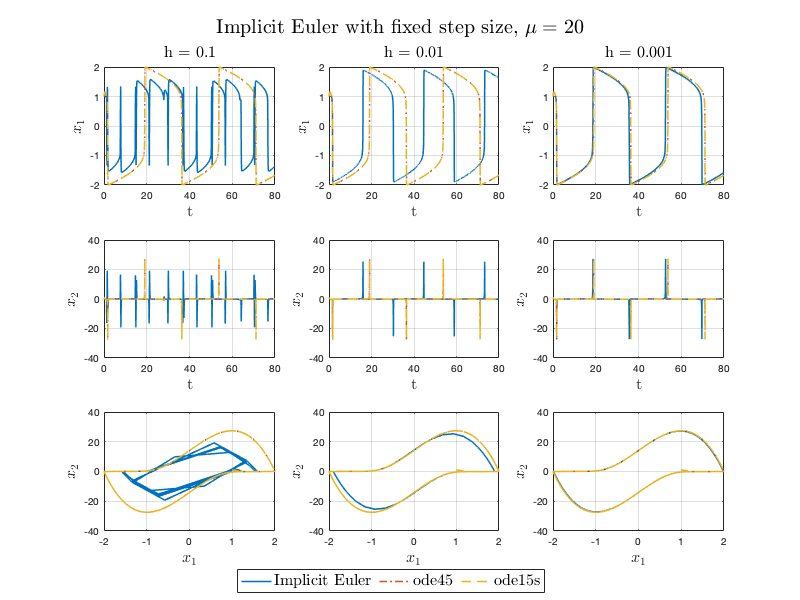
\includegraphics[width=\textwidth]{graphics/opg3/mu20_fixed.png}
    \caption{Solution to Van der Pol with $\mu = 20$ using fixed step sizes}
    \label{fig3:fixed_mu20}
\end{figure}

Table \ref{tab3:mu20_fixed} shows that CPU time and number of function evaluations when solving the Van der Pol problem with $\mu = 20$ using different time steps and Matlab ODE solvers. Notice that with $h=0.1$ the implicit Euler is as fast as any of the other methods, however, as seen above the results are also completely wrong. A time step of $h=0.01$ yields similar run time to ODE15s---but with substantial deviations in the results. A step size of $h=0.001$ is by far the slowest of the methods, and the one that uses the most function evaluations. One of the reasons why ODE45 and ODE15s are able to outperform the implicit Euler with fixed step size is because they are able to adjust the step size such that a larger step size is used in the parts with a slower dynamic and vice versa. 

Notice that ODE45 does not outperform ODE15s anymore. This is a good indication that the problem is stiff, i.e., it is worth while to use an implicit method that even when it comes with additional computational cost. The implicit method is also able to use far less function evaluations than the DoPri54. 

\begin{table}[H]
    \centering
    \caption{CPU time and function evaluations of implicit Euler with fixed time step and Matlab ODE solvers}
    \begin{tabular}{|c||c|c|c|c|c|c|} \hline
         \textbf{Method}    & $h=0.1$&   $h=0.01$ & $h=0.001$ & ODE45 & ODE15s     \\ \hline \hline 
         \textbf{Time}      & 0.0325  &  0.0691  &  0.3027 & 0.0370 & 0.0504   \\ \hline
         \textbf{Fun evals} & 7001    &   33175   &   199129 & 8461 & 926  \\ \hline
    \end{tabular}
    \label{tab3:mu20_fixed}
\end{table}



Figure \ref{fig3:adap_mu20} shows the numerical solution to the Van der Pol problem with $\mu = 20$ for implicit Euler with adaptive time steps and $AbsTol=RelTol \in \{10^{-2}, 10^{-4}, 10^{-6}\}$, ODE45 and ODE15s. Notice also that for $Tol = 10^{-2}$ there is a quite big difference between the implicit Euler solution and the other solutions; for $Tol = 10^{-4}$ the difference is almost not visible and for $Tol = 10^{-6}$ there is no visible difference anymore.

\begin{figure}[H]
    \centering
    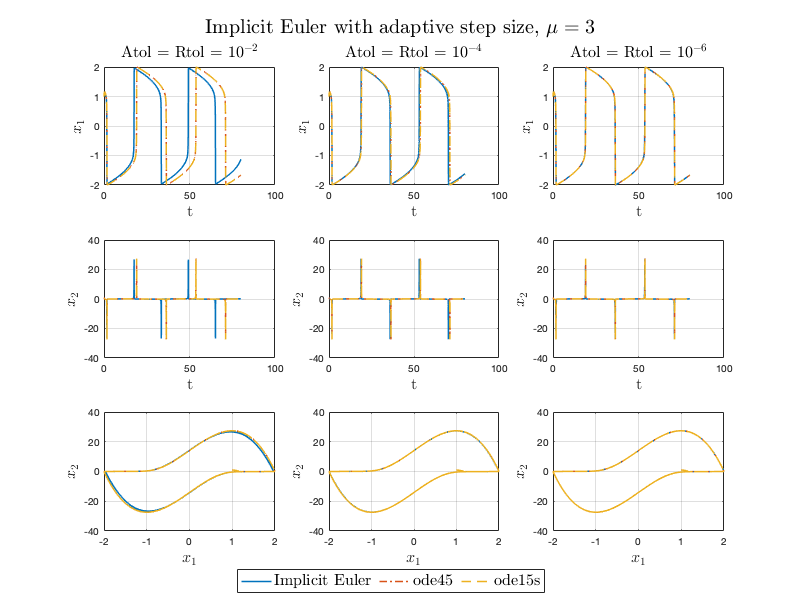
\includegraphics[width=\textwidth]{graphics/opg3/mu20_adap.png}
    \caption{Solution to Van der Pol with $\mu = 20$ using adaptive step sizes}
    \label{fig3:adap_mu20}
\end{figure}

Table \ref{tab3:mu20_adap} shows that CPU time and number of function evaluations when solving the Van der Pol problem with $\mu = 20$ using different tolerances and Matlab ODE solvers. Notice that with $Tol = 10^{-2}$ the implicit Euler is already slower than Matlab ODE solvers, and as seen above the results also deviate from the rest. Using $Tol = 10^{-4}$ yields even higher run time, but now with very little deviation in the results. Finally $Tol = 10^{-6}$ is by far the slowest of the methods, and the one that uses the most function evaluations (by a quite substantial amount). 

One of the reasons why ODE45 and ODE15s are able to outperform the implicit Euler with adaptive step size is because they are higher order methods and because they are implemented very very efficiently. 

\begin{table}[H]
    \centering
    \caption{CPU time and function evaluations of implicit Euler with adaptive time step and Matlab ODE solvers}
    \begin{tabular}{|c||c|c|c|c|c|c|} \hline
         \textbf{Method}    & $Tol = 10^{-2}$&   $Tol = 10^{-4}$ & $Tol = 10^{-6}$ & ODE45 & ODE15s     \\ \hline \hline 
         \textbf{Time}      & 0.1045 &    0.4818 &    0.8793 & 0.0386 & 0.0612   \\ \hline
         \textbf{Fun evals} &  21977 &  46903 &      446091 & 8461 & 2944  \\ \hline
    \end{tabular}
    \label{tab3:mu20_adap}
\end{table}

Figure \ref{fig3:adap_mu20_h} shows the used step sizes for the different tolerances. The red crosses mark whenever the step size controller failed to set the step size correctly, i.e., whenever the estimated (using step doubling) error was larger than the allowed maximum. Notice that the behaviour of all three tolerances are quite similar. Also notice that the step sizes vary by more than a factor 1000! This is a good indication that the problem is stiff. Also notice that for $AbsTol=RelTol=10^{-2}$ the step size controller fails at setting the correct step size many times. This again indicates that there is a rapid change in dynamics, which leads to a large needed change in step size---larger than anticipated by the step size controller.

\begin{figure}[H]
    \centering
    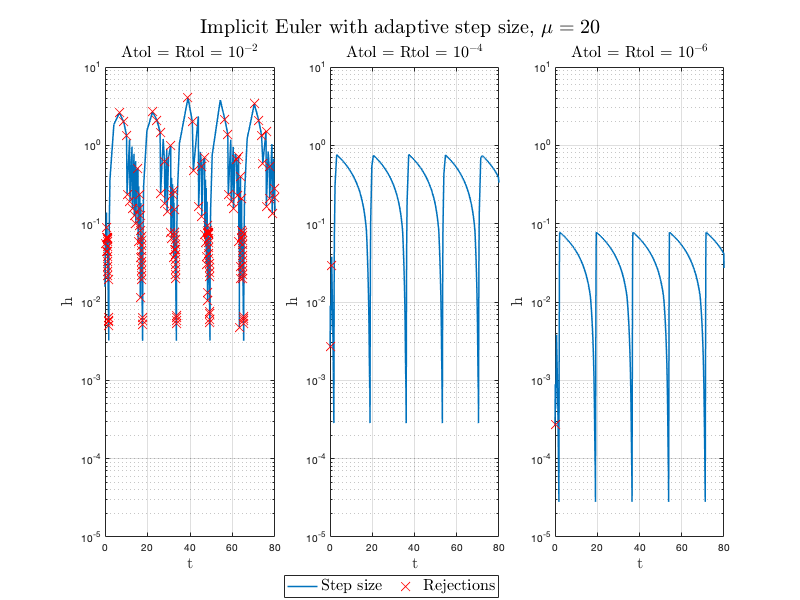
\includegraphics[width=\textwidth]{graphics/opg3/mu20_h.png}
    \caption{Step sizes when solving the Van der Pol with $\mu = 20$ at different tolerances}
    \label{fig3:adap_mu20_h}
\end{figure}







\clearforchapter
\chapter{Solvers for SDEs}
We now consider the stochastic differential equation (SDE) on the form

\begin{align}
    dx(t) &= f(t,x(t),p_f)dt + g(t,x(t),p_g)d\omega(t) \\
    d\omega & \sim N_{iid}(0,I dt)
\end{align}

where $x\in \probR^{n_x}$ and $\omega$ is Brownian motion with dimension $n_\omega$. $p_f$ and $p_g$ are parameters for the drift and the diffusion term respectively. 

\section{Multivariate Wiener process}
Before we can start simulating any SDEs, we need to have a way of generating realizations of Brownian motion. Brownian motion is defined as the integral of \textit{random noise}, which is a complex mathematical construction that does not exist in real life. Furthermore, Brownian motion is a fractal, meaning that its behaviour is scale indifferent, i.e., if you "zoom in" the pattern repeats itself indefinitely. Brownian motion is defined as a continuous function with mean $0$, and variance $t$. Brownian motion was discovered by the English botanist, Brown, as he saw pollen moving due to molecules bumping into each other. This later lead to the discovery of molecules, and precise estimation of the number of molecules in a mole. Sometimes Brownian motion is called \textit{the Wiener process}, hence we might denote it $\omega$. Listing \ref{lst4:bm} is a Matlab implementation of a function that simulates a realization of a multivariate Brownian motion. 

\begin{lstlisting}[language=Matlab,caption=Simulation of multivariate Brownian motion,label=lst4:bm]
function [W,Tw,dW] = StdWienerProcess(T,N,nW,Ns,seed)
    % StdWienerProcess Ns realizations of a standard Wiener process
    %
    % Syntax: [W,Tw,dW] = StdWienerProcess(T,N,Ns,seed)
    % W : Standard Wiener process in [0,T]
     %Tw : Time points
     %dW : White noise used to generate the Wiener process
    %
    % T : Final time
    % N : Number of intervals
    % nW : Dimension of W(k)
    % Ns : Number of realizations
    % seed : To set the random number generator (optional)
    if nargin == 4
        rng(seed);
    end
    dt = T/N;
    dW = sqrt(dt)*randn(nW,N,Ns);
    W = [zeros(nW,1,Ns) cumsum(dW,2)];
    Tw = 0:dt:T;
\end{lstlisting}

Figure \ref{fig4:2dBM} shows three realizations of 2D standard Brownian motion. 

\begin{figure}[H]
    \centering
    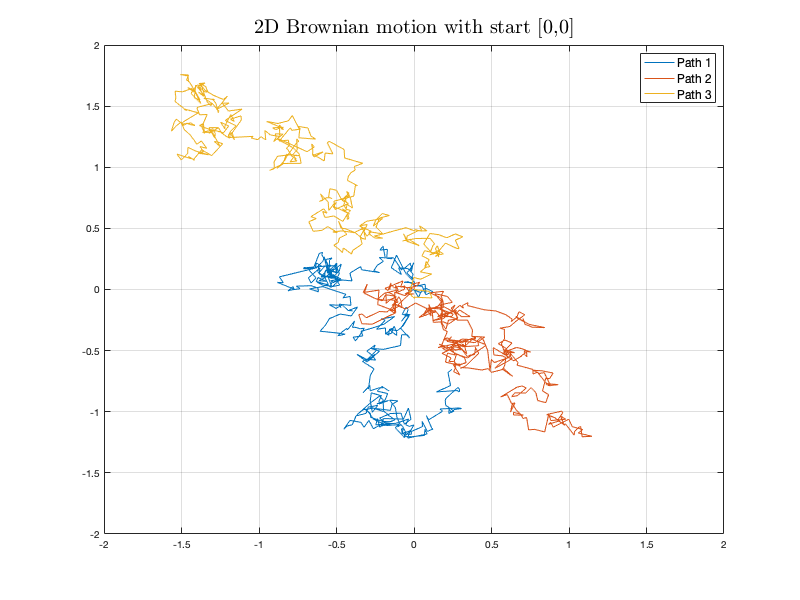
\includegraphics[width=\textwidth]{graphics/opg4/2dBM.png}
    \caption{Three realizations of 2D standard Wiener process}
    \label{fig4:2dBM}
\end{figure}



\section{Implementation of Euler-Manayam}
Given a SDE, we want to be able to simulate sample paths. To do this, we need to be able to solve the SDE numerically. Generally, speaking SDEs are often solved by the stochastic analogue to the explicit Euler method, i.e., 1. order Taylor with left-bound starting point, to solve the stochastic part. In fact, this is so pronounced that there is an entire algebra that is based on this principle known as It$\Bar{\text{o}}$ calculus, after the Japanese mathematician. 

The first approach, and perhaps most natural, is to use explicit Euler for both the drift and the diffusion term. This is known as the explicit-explicit method or alternatively \textit{Euler-Manayama}. The method is based upon

\begin{align}
    x(t+h) - x(t) &= f(t,x(t),p_f)h + g(t,x(t),p_g)(\omega(t+h)-\omega(t)) \\
    x(t+h) &= x(t) + f(t,x(t),p_f)h + g(t,x(t),p_g)(\omega(t+h)-\omega(t)).
\end{align} 

Listing \ref{lst4:EE} shows the Matlab implementation of the explicit-explicit method.


\begin{lstlisting}[language=Matlab,caption=Implementation of Euler-Manayama,label=lst4:EE]
function [x,f,J] = SDENewton(ffun,t,dt,psi,xinit,tol,maxit,varargin)
    I = eye(length(xinit));
    x = xinit;
    [f,J] = feval(ffun,t,x,varargin{:});
    R = x - f*dt - psi;
    it = 1;
    while ( (norm(R,'inf') > tol) && (it <= maxit) )
        dRdx = I - J*dt;
        mdx = dRdx\R;
        x = x - mdx;
        [f,J] = feval(ffun,t,x,varargin{:});
        R = x - f*dt - psi;
        it = it+1;
    end
\end{lstlisting}



\section{Implementation of implicit-explicit}
Another approach to solving the SDE is to combine an implicit and an explicit method. To maintain the consistency wrt ordinary stochastic calculus the diffusion term is still treated by an explicit method, however, the drift term is now solved by an implicit Euler method. Hence the method is based upon

\begin{align}
    x(t+h) - x(t) = f(t+h,x(t+h),p_f)h + g(t,x(t),p_g)(\omega(t+h)-\omega(t)) \\
    x(t+h) - x(t) - f(t+h,x(t+h),p_f)h - g(t,x(t),p_g)(\omega(t+h)-\omega(t)) = 0.
\end{align} 

The latter can be solved by using Newton method (alternatively inexact Newton). Listing \ref{lst4:IE} shows the Matlab implementation of the implicit-explicit method.

\begin{lstlisting}[language=Matlab,caption=Implementation of the implicit-explicit method for SDEs,label=lst4:IE]
function X=SDEimplicit(ffun,gfun,T,x0,W,varargin)
    tol = 1.0e-8;
    maxit = 100;

    N = length(T);
    nx = length(x0);
    X = zeros(nx,N);

    X(:,1) = x0;
    k=1;
    [f,~] = feval(ffun,T(k),X(:,k),varargin{:});

    for k=1:N-1
        g = feval(gfun,T(k),X(:,k),varargin{:});
        dt = T(k+1)-T(k);
        dW = W(:,k+1)-W(:,k);
        psi = X(:,k) + g*dW;
        xinit = psi + f*dt;
        [X(:,k+1),f,~] = SDENewton(ffun, T(:,k+1), dt, psi, xinit, tol, maxit, varargin{:});
    end
\end{lstlisting}


\section{Test on stochastic Van der Pol}
Now that we have made an implementation of the both and explicit-explicit and an implicit-explicit method with fixed step size we want to compare these. To do so we look at the Van der Pol problem given by
\begin{align}
    \Ddot{x}(t) &= \mu (1-x(t)^2) \dot{x}(t) - x(t).
\end{align}
To solve the problem using the explicit Euler method we must first re-write the problem as a system of first order differential equations. Luckily this is done easily and given by

\begin{align}
    \dot{x}_1(t) &= x_2(t) \\
    \dot{x}_2(t) &= \mu(1-x_1(t)^2) x_2(t) - x_1(t).
\end{align}

Since we are looking at SDEs, we will use a stochastic version of the system. Van der Pol with state \textit{independent} diffusion is given by

\begin{align}
    dx_1(t) &= x_2(t)dt \\
    dx_2(t) &= \left[\mu(1-x_1(t)^2) x_2(t) - x_1(t)\right] dt + \sigma d\omega (t).
\end{align}

The Van der Pol problem with state \textit{dependent} diffusion is given by

\begin{align}
    dx_1(t) &= x_2(t)dt \\
    dx_2(t) &= \left[\mu(1-x_1(t)^2) x_2(t) - x_1(t)\right] dt + \sigma\left(1+ x_1(t)^2\right) d\omega (t).
\end{align}

We will now test the explicit Euler method on the Van der Pol problem with $\mu \{3,20\}$,  $x_1(0)=x_2(0)=0.5$ and $\sigma \in \{1,2\}$, with both state dependent and state independent diffusion terms.

\subsection{Explicit-explicit}
Figure \ref{fig4:ex_indep} shows realization of solution to the stochastic Van der Pol problem with state independent diffusion solved with Euler-Manayama. From the plot it is evident that faster dynamic given when $\mu=20$ reduce the relative effect of the diffusion term. Therefore, the system with $\mu=20$ exhibit less stochastic behaviour.

It is also evident that increasing the diffusion parameter, $\sigma$, increases the stochasticity in the system. The realization with high diffusion parameter have visibly more variance. 

\begin{figure}[H]
    \centering
    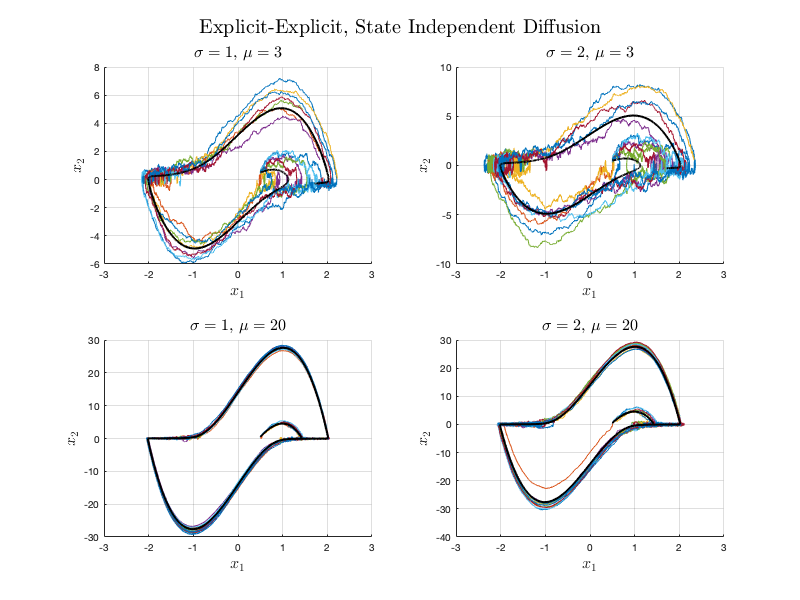
\includegraphics[width=\textwidth]{graphics/opg4/ex_indep.png}
    \caption{Explicit-explicit solution with state independent diffusion}
    \label{fig4:ex_indep}
\end{figure}


Figure \ref{fig4:ex_dep} shows realization of solution to the stochastic Van der Pol problem with state dependent diffusion again solved with Euler-Manayama. From the plot we can see quite different behaviour compared with the realizations for state independent diffusion. Specifically, the stochasticity is more pronounced when $|x_1|$ is large, i.e., in the left- and right hand side of the plots.  

This time the effect of increasing the diffusion parameter, $\sigma$, increases the stochasticity in the system even more than before. Before we mainly saw a difference in variance for the low value of $\mu$. This time we also see a big difference where $\mu=20$.

\begin{figure}[H]
    \centering
    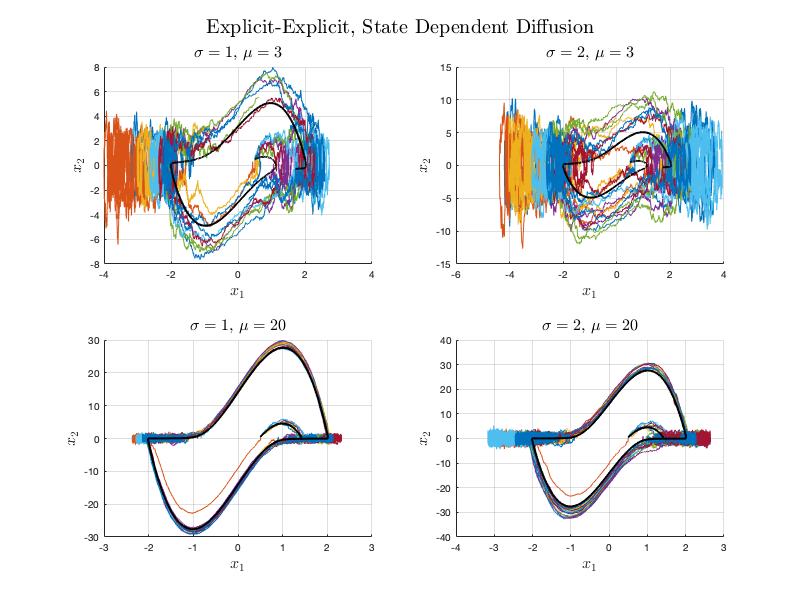
\includegraphics[width=\textwidth]{graphics/opg4/ex_dep.png}
    \caption{Explicit-explicit solution with state dependent diffusion}
    \label{fig4:ex_dep}
\end{figure}

\subsection{Implicit-explicit}
Figure \ref{fig4:im_indep} shows realization of solution to the stochastic Van der Pol problem with state independent diffusion solved with an implicit-explicit method. From the plot it is evident that faster dynamic given when $\mu=20$ reduce the relative effect of the diffusion term. Therefore, the system with $\mu=20$ exhibit less stochastic behaviour.

It is also evident that increasing the diffusion parameter, $\sigma$, increases the stochasticity in the system. The realization with high diffusion parameter have visibly more variance. 

\begin{figure}[H]
    \centering
    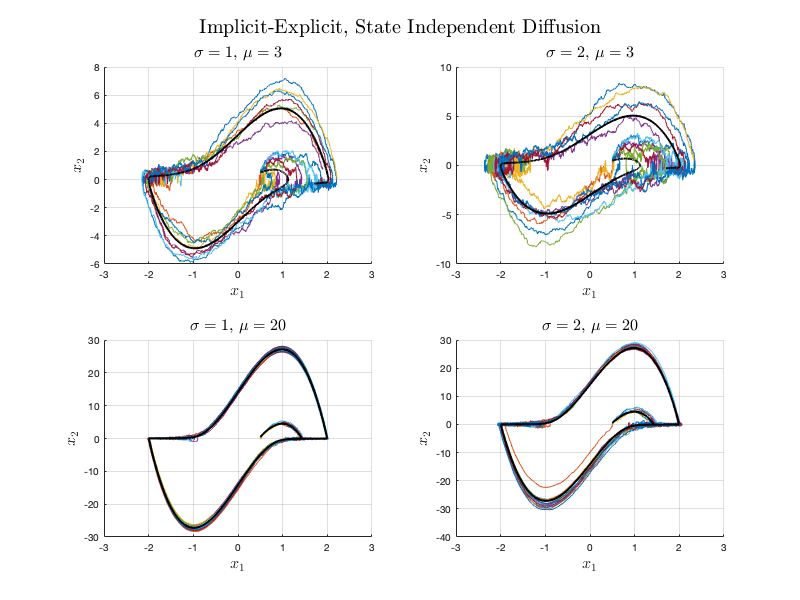
\includegraphics[width=\textwidth]{graphics/opg4/im_indep.png}
    \caption{Implicit-explicit solution with state independent diffusion}
    \label{fig4:im_indep}
\end{figure}


Figure \ref{fig4:im_dep} shows realization of solution to the stochastic Van der Pol problem with state dependent diffusion again solved with an implicit-explicit method. From the plot we can see quite different behaviour compared with the realizations for state independent diffusion. Specifically, the stochasticity is more pronounced when $|x_1|$ is large, i.e., in the left- and right hand side of the plots.  

This time the effect of increasing the diffusion parameter, $\sigma$, increases the stochasticity in the system even more than before. Before we mainly saw a difference in variance for the low value of $\mu$. This time we also see a big difference where $\mu=20$.

Overall, the difference between the solutions with the explicit-explicit and implicit-explicit method is very small. By visual inspections of the realization it is not possible to tell the solution curves apart---however, for particularly stiff systems the implicit-explicit method might not require as many function calls. 


\begin{figure}[H]
    \centering
    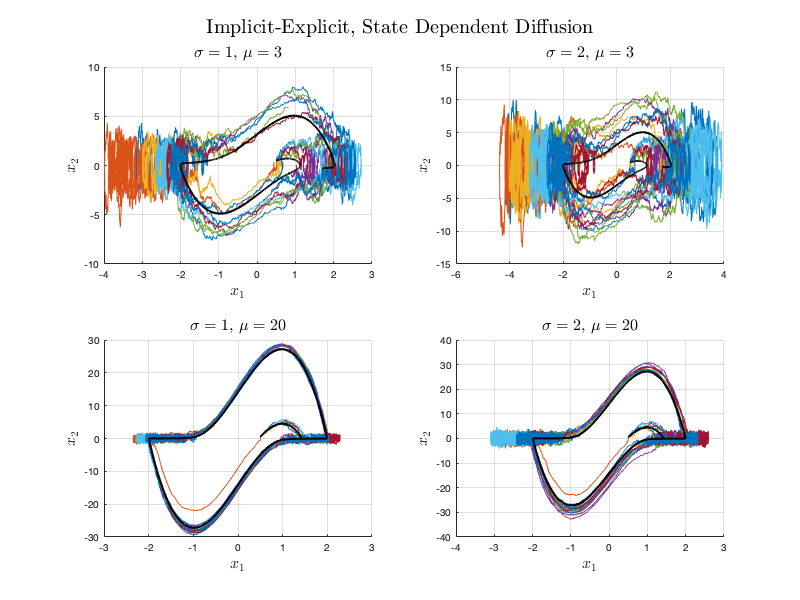
\includegraphics[width=\textwidth]{graphics/opg4/im_dep.png}
    \caption{Implicit-explicit solution with state dependent diffusion}
    \label{fig4:im_dep}
\end{figure}


\subsection{Weak vs strong convergence}
Generally, the goal of numerical methods is to approximate systems of differential equation as good as possible with as little computational cost as possible. A requirement for such numerical methods is some consistency, i.e., the approximation should become arbitrarily good when the step size becomes arbitrarily small. To this end, we have introduced the notion of \textit{order}. 

We say that a method as order $p$ whenever $e = \mathcal{O}(h^p)$, where $e$ is the errors and $h$ is the step size. Naturally, we want the order to be as big as possible (we generally use $h<1$). However, for stochastic methods it is not as simple. For stochastic systems we can measure both the accuracy of the mean, known as \textit{strong convergence}. Alternatively, we can measure the accuracy of the statistics of the individual trajectories at the end point---known as \textit{weak convergence}. 

Euler-Manayama has weak order 1, but only strong order 0.5. This means that for very noisy systems, we might require a very low step size. Figure \ref{fig4:sde_order} shows solutions to realizations to the stochastic Van der Pol together with solution to the deterministic system. Notice that for the same step size the stochastic system might diverge while the deterministic does not. This is because of the difference between the strong and weak convergence of the Euler-Manayama scheme. 

\begin{figure}[H]
    \centering
    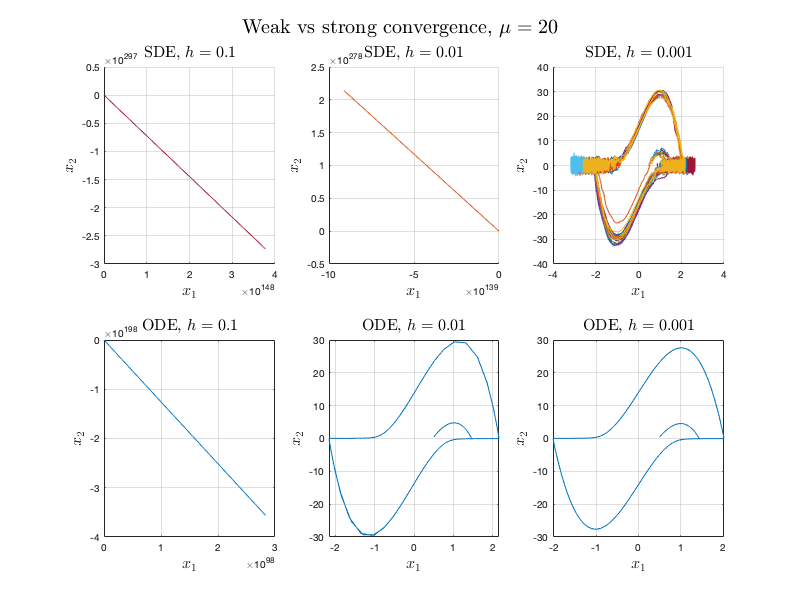
\includegraphics[width=\textwidth]{graphics/opg4/sde_order.png}
    \caption{Implicit-explicit solution with state dependent diffusion}
    \label{fig4:sde_order}
\end{figure}






\clearforchapter
\chapter{Classical Runge-Kutta}
In the following, we go back to considering the initial value problem (IVP) on the form
\begin{align}
    \dot{x}(t) &= f(t,x(t),p), & x(t_0) = x_0,
\end{align}
where $x \in \probR ^{n_x}$ and $p \in \probR ^{n_p}$. 

\section{Description of the classical Runge Kutta}
We have previously seen how to use the explicit- or implicit Euler method to solve IVPs. Both of these are first order methods, meaning that their global truncation errors will be directly proportional to the step size of the method, as described in chapter 1. We will now consider a slightly more elaborate method, namely the classical Runge-Kutta method (RK4). 

Again, we wish to determine $x(t+h), \ h>0$ when we know $x(t)$. Via the fundamental theorem of calculus, we have

\begin{align}
    x(t+h) &= x(t) + \int_{t}^{t+h} \dot{x}(t,x(t)) dt.
\end{align}

Notice that our goal now boils down to determining 

\begin{align}
\int_{t}^{t+h} \dot{x}(t,x(t)) dt, \quad h > 0.
\end{align}

If we remember our basic courses in calculus, we remember that there exits many ways to approximate such an integral. The simplest methods are probably the left or right point methods. These correspond to using explicit- or implicit Euler method. The next step is to use the midt point method 

\begin{align}
    x(t+h) &= x(t) + h \cdot \dot{x}\left (t+\frac{h}{2}, x\left (t+\frac{h}{2}\right) \right).
\end{align}

Another is the trapezoidal method

\begin{align}
    x(t+h) &= x(t) + \frac{h}{2} \cdot \dot{x}\left (t, x\left (t\right) \right) + \frac{h}{2} \cdot \dot{x}\left (t+h, x\left (t+h\right) \right).
\end{align}

Notice that this method use a second order Taylor to approximate $x(t)$, which results in integral of an affine function. We could take it one step further and use Simpson's rule, i.e., taking the integral of the approximating quadratic function, then we would get

\begin{align}
    x(t+h) &= x(t) + \frac{h}{6} \left( \dot{x}\left (t, x\left (t\right) \right) + 4 \dot{x}\left (t+ \frac{h}{2}, x\left (t+\frac{h}{2}\right) \right) +\dot{x}\left (t+h, x\left (t+h\right) \right) \right).
\end{align}

Using this approximation, we get what is known as the classical Runge-Kutta method (RK4). The method relies on a non-linear approximation of the original function, as such it approximates it better than first order methods. In fact, RK4 is or order 4\cite{Ascher}. So we have

\begin{align}
    x(t+h) &= x(t) + \frac{h}{6} \left( \dot{x}\left (t, x\left (t\right) \right) + 4 \cdot ...  \right) + \mathcal{O}(h^5).
\end{align}

Now we have the intuition on how RK4 works, however, notice that we do not have all elements on the right hand side. We will therefore dig into how we actually use these methods. In practice, we define for a $s$ stage Runge-Kutta method 

\begin{align}
    T_i &= t_n+c_i \cdot h, \quad i = \{1,2,...,s\}\\
    X_i &= x_n + h \cdot \sum_{j=i}^{s} a_{ij} f(T_j, X_j), \quad i = \{1,2,...,s\},
\end{align}
and
\begin{align}
    t_{n+1} &= t_n + h \\
    x_{n+1} &= x_n + h \cdot \sum_{i=1}^s b_i f(T_i,X_i)
\end{align}
where $x_n=x(t_n)$. We see that the $c_i$'s are used to determine the intermediate time points. The $a_i$'s scale how important each slope estimate is for the individual stages. Finally, the $b_i$'s weights the slopes in relation to the total slope estimate. Often, and for simplicity, we show the parameters in a \textit{butcher tableau}

\begin{align}
    \begin{array}{c|cccc}
         c_1 & & & &   \\
         c_2 & a_{21} & & & \\
         \vdots & \vdots  & \vdots & & \\
         c_s & a_{s1} & a_{s2} & \cdots & \\ \hline 
         x & b_1 & b_2 & \cdots & b_s
    \end{array}
\end{align}
The method is said to be consistent iff we have
\begin{align}
    \sum b_1 = 1.
\end{align}

For the classical Runge-Kutta method, the butcher tableau is given by

\begin{align}
    \begin{array}{c|cccc}
         0   & & & &   \\
         1/2 & 1/2 & & & \\
         1/2 & 0 & 1/2 & & \\
         1   & 0 & 0   & 1 & \\ \hline 
         x   & 1/6 & 1/3 & 1/3 & 1/6.
    \end{array}
\end{align}

The RK4 method is not A- nor L-stable. Figure \ref{fig1:rk4_stability} shows the stability region of RK4 on the test equation. 


\section{Classical Runge Kutta fixed time step implementation}
We now have all theory in place such that we can start using RK4. Listing \ref{lst5:rk4_fixed} shows a Matlab implementation of an explicit Runge-Kutta solver with fixed time step. Notice that to use RK4, we must use the parameters from the butcher tableau. These can be seen in the code below the solver. 

\begin{lstlisting}[language=Matlab,caption=Implementation of explicit Runge-Kutta solver. Parameters corresponding to RK4 given at the end,label=lst5:rk4_fixed]
function [x,t,function_calls,hs] = explicitRungeKutta(f,param,h,t0,T,x0,A,b,c)
    N = ceil((T-t0)/h);
    t = zeros(1,N+1);
    hs = ones(1,N+1);
    hs = h.*hs;
    x = zeros(length(x0),N+1);
    s = length(b);
    k = zeros(length(x0),s)';
    t(1) = t0;
    x(:,1) = x0;
    function_calls = 0;
    
    Ah = h*A;
    bh = h*b;
    ch = h*c;
    
    for i = 2:N+1
       if t(i-1)+h > T
            h = T-t(i-1);
       end
       k = 0*k;
       for j = 1:s
           k(j,:) = f(t(i-1)+ch(j),x(:,i-1)+sum(k.*Ah(j,:)',1)', param);
           function_calls = function_calls +1;
       end
       x(:,i) = x(:,i-1)+sum(k.*bh,1)';
       t(i) = t(i-1)+h;
    end
    x = x';
end

%% RK4 paramters:
A = [0 0 0 0; 0.5 0 0 0; 0 0.5 0 0; 0 0 1 0];
b = [1/6 2/6 2/6 1/6]';
c = [0 1/2 1/2 1]';
p = 4;
\end{lstlisting}


\section{Classical Runge Kutta adaptive time step implementation}
As discussed in previous chapters it can be difficult to select a suitable step size, $h$. When dealing with more advanced problems, particularly stiff problems, we might see that a smaller step size might be required in parts of the solution than others. This problem leads to a desire to construct an algorithm that can change the step size adaptively. The goal is to use as large step size as possible, while maintaining a sufficient accuracy in the individual steps. 

We will again use \textit{step doubling} to estimate the one step errors of the methods, as described in previous chapters. Once again, we are able to define how to select the best step size, $h$. We do so by using the \textit{asymptotic step size controller}. Since RK4 is a 4th order method this means that our step size is given by
\begin{align}
    h_{k+1} &= \left(\frac{\varepsilon}{r_{k+1}} \right )^{1/5} h_k.
\end{align}
Where $r_{k+1}$ is found by
\begin{align}
    r_{k+1} &= \max_{i \in \{1,...,n_x\}} \left \{ \frac{|e_{k+1}|_i}{ \max \{ |\text{abstol}|_i, \ |x_{k+1}|_i \cdot |\text{reltol}|_i \} } \right \}
\end{align}
where $|\text{abstol}|_i$ and $|\text{reltol}|_i$ are the absolute and relative tolerance of $(x_{k+1})_i$ respectively.

Listing \ref{lst5:rk4_adap} shows a Matlab implementation of a general Runge-Kutta solver with error estimation using step doubling and asymptotic step size controller. As before, the specific parameters for RK4 are given below the solver. 

\begin{lstlisting}[language=Matlab,caption=Implementation of explicit Runge-Kutta solver with adaptive time step. Parameters corresponding to RK4 given at the end,label=lst5:rk4_adap]
function [x,t,function_calls,hs] = explicitRungeKuttaDoubling(f,param,h,t0,T,x0,A,b,c,Atol,Rtol,hmin,hmax,eps_tol,p,initial_step_algo)
    N = ceil((T-t0)/hmin);
    s = length(b);
    d = length(x0);
    t = zeros(1,N+1);
    hs = zeros(1,N+1);
    x = zeros(length(x0),N+1);
    k = zeros(d,s)';
    t(1) = t0;
    x(:,1) = x0;
    accept_step = false;
    function_calls = 0;
    
    if initial_step_algo % slide 4b, 9 whic is from p169 Hairer
        [h,function_calls] = initialStepSize(f,param,t0,x0);
    end
    
    i = 2;
    while t(i-1)<=T
       while(~accept_step)
           if t(i-1)+h>T
               h = max(hmin,T-t(i-1));
           end
           
           k = 0*k;
           for j = 1:s
               k(j,:) = f(t(i-1)+h*c(j),x(:,i-1)+sum(h*k.*A(j,:)',1)', param);
               function_calls = function_calls +1;
           end
           oneAhead = x(:,i-1)+sum(h*k.*b,1)';

           hhalf = h/2;
           k = 0*k;
           for j = 1:s
               k(j,:) = f(t(i-1)+hhalf*c(j),x(:,i-1)+sum(hhalf*k.*A(j,:)',1)', param);
               function_calls = function_calls +1;
           end
           halfAhead = x(:,i-1)+sum(hhalf*k.*b,1)';

           k = 0*k;
           for j = 1:s
               k(j,:) = f(t(i-1)+2*hhalf*c(j),halfAhead+sum(hhalf*k.*A(j,:)',1)', param);
               function_calls = function_calls +1;
           end
           halfAhead = halfAhead+sum(hhalf*k.*b,1)';
           
           % Step doubling, see section II.4(s164) in Harier and slide 4c,3
           e = abs(oneAhead-halfAhead);
           r = max(e./max(Atol,abs(halfAhead).*Rtol));
           
           if r<=1
               x(:,i) = halfAhead;
               hs(i-1) = h;
               t(i) = t(i-1)+h;
               accept_step = true;
           else
               accept_step = false;
           end
           h = h*max(hmin,min(hmax,(eps_tol/r)^(1/(1+p)))); % eq 4.13 in Harier
       end
       accept_step = false;
       i = i+1;
    end
    x = x(:,1:i-1)';
    t = t(1:i-1);
    hs = hs(1:i-2);
end

%% RK4 paramters:
A = [0 0 0 0; 0.5 0 0 0; 0 0.5 0 0; 0 0 1 0];
b = [1/6 2/6 2/6 1/6]';
c = [0 1/2 1/2 1]';
p = 4;
\end{lstlisting}


\section{Test on Van der Pol problem and comparison with Matlab ODE solvers}
Now that we have made an implementation of the classical Runge Kutta method with both fixed and adaptive step size we want to compare these. To do so we look at the Van der Pol problem given by
\begin{align}
    \Ddot{x}(t) &= \mu (1-x(t)^2) \dot{x}(t) - x(t).
\end{align}
To solve the problem we must first re-write the problem as a system of first order differential equations. Luckily this is done easily and given by
\begin{align}
    \dot{x}_1(t) &= x_2(t) \\
    \dot{x}_2(t) &= \mu(1-x_1(t)^2) x_2(t) - x_1(t).
\end{align}

We will now test the classical Runge Kutta method on the Van der Pol problem with $\mu = 3$ and $\mu = 20$. 

\subsection{Van der Pol, $\mu = 3$}
The Van der Pol problem with $\mu = 3$ is a relatively straight forward non-stiff problem. There is no formal definition of when a problem is \textit{stiff}---only that whenever a problem change dynamics "very quickly" it is said to be. 

Figure \ref{fig5:fixed_mu3} shows the numerical solution to the Van der Pol problem with $\mu = 3$ for RK4 with $h \in \{0.1, 0.01, 0.001\}$, ODE45 and ODE15s. Notice that there is no visible difference between the solution obtained by ODE45 and ODE15s. Notice also that for already for $h=0.1$ there is almost no difference between RK4 and ODE45/ODE15s. If we look very closely, we can see some small local deviation in the line, however, they are actually not because the method is wrong, the distance between the estimated points are just so big, that we can see the straight line Matlab draws between them. It seems that this problem is an easy task for the RK4 method, even with relatively large step sizes.

\begin{figure}[H]
    \centering
    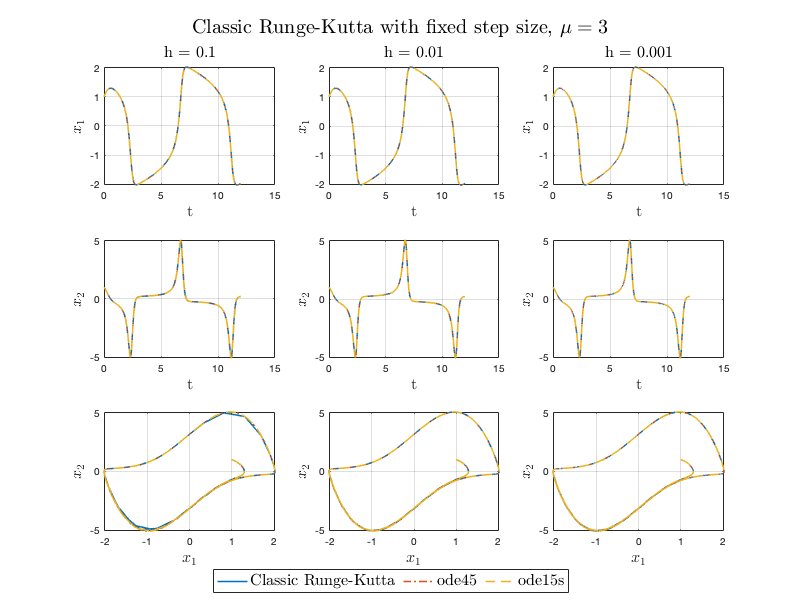
\includegraphics[width=\textwidth]{graphics/opg5/mu3_fixed.png}
    \caption{Solution to Van der Pol with $\mu = 3$ using fixed step sizes}
    \label{fig5:fixed_mu3}
\end{figure}

Table \ref{tab5:mu3_fixed} shows that CPU time and number of function evaluations when solving the Van der Pol problem with $\mu = 3$ using different time steps and Matlab ODE solvers. Notice that with $h=0.1$ the RK4 uses the fewest function calls of any of the methods. Even so, the ODE45 is still as fast---which might be a bit surprising. The issue here is that when we call our own function, they are made in Matlab. Therefore there will be some overhead on the run time. This has been minimized on the build in functions, which makes the Matlab function very difficult to beat when comparing run-times. 

Notice that ODE45 seems to outperform ODE15s. This is a good indication that the problem is not particular stiff, i.e., it is not worth while to use an implicit method that comes with additional computational cost. 

\begin{table}[H]
    \centering
    \caption{CPU time and function evaluations of classical Runge Kutta with fixed time step and Matlab ODE solvers}
    \begin{tabular}{|c||c|c|c|c|c|c|} \hline
         \textbf{Method}    & $h=0.1$&   $h=0.01$ & $h=0.001$ & ODE45 & ODE15s     \\ \hline \hline 
         \textbf{Time}      & 0.0042 &   0.0196 &   0.2029 &  0.0046 & 0.0175   \\ \hline
         \textbf{Fun evals} & 480     &   4800   &    48000 & 1069 & 926  \\ \hline
    \end{tabular}
    \label{tab5:mu3_fixed}
\end{table}



Figure \ref{fig5:adap_mu3} shows the numerical solution to the Van der Pol problem with $\mu = 3$ for the classical Runge Kutta with adaptive time steps and $AbsTol=RelTol \in \{10^{-2}, 10^{-4}, 10^{-6}\}$, ODE45 and ODE15s. Notice also that for $Tol = 10^{-2}$ we again see some difference in the plots. Once again, it is simply because at the tolerance, the RK4 take such large time steps, that we can see the straight lines by Matlab. This is especially visible in the "corner" of the solution curve.

\begin{figure}[H]
    \centering
    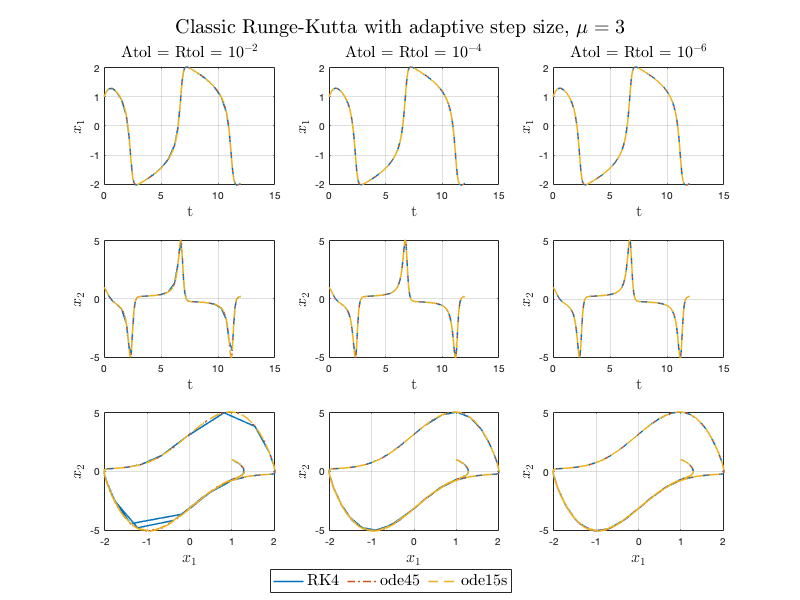
\includegraphics[width=\textwidth]{graphics/opg5/mu3_adap.png}
    \caption{Solution to Van der Pol with $\mu = 3$ using adaptive step sizes}
    \label{fig5:adap_mu3}
\end{figure}

Table \ref{tab5:mu3_adap} shows the CPU time and number of function evaluations when solving the Van der Pol problem with $\mu = 3$ using different tolerances and Matlab ODE solvers. Notice that with $Tol = 10^{-2}$ the RK4 is relatively fast (slower than ODE45 but as fast as ODE15s). Generally, it is very hard to tell the solutions curves apart just by looking at them. Even for the lowest tolerance, we get quite good results. What is interesting is the CPU time usage and number of function evaluations used at the different tolerances. For both explicit- and implicit Euler, we saw that the CPU time and function evaluations increased dramatically when we required higher accuracy, now this increase is not as pronounced. This demonstrates the power of higher order methods quite well.

One of the reasons why ODE45 is able to outperform the RK4 with adaptive step size is because it used an embedded error estimate, i.e., not step doubling. Using an embedded error estimate is a more efficient way of estimating the errors and hence the algorithm is faster.

\begin{table}[H]
    \centering
    \caption{CPU time and function evaluations of RK4 with adaptive time step and Matlab ODE solvers}
    \begin{tabular}{|c||c|c|c|c|c|c|} \hline
         \textbf{Method}    & $Tol = 10^{-2}$&   $Tol = 10^{-4}$ & $Tol = 10^{-6}$ & ODE45 & ODE15s     \\ \hline \hline 
         \textbf{Time}      & 0.0209 &   0.0622 &    0.0577 & 0.0046 & 0.0175   \\ \hline
         \textbf{Fun evals} & 758   &     1562   &     3374 & 1069 & 926  \\ \hline
    \end{tabular}
    \label{tab5:mu3_adap}
\end{table}

Figure \ref{fig5:adap_mu3_h} shows the used step sizes for the different tolerances. The red crosses mark whenever the step size controller failed to set the step size correctly, i.e., whenever the estimated (using step doubling) error was larger than the allowed maximum. Notice that the behaviour of all three tolerances are quite similar. Also notice that the step sizes does not vary nearly as much for the individual tolerances as previously seen (for explicit- and implicit Euler). Additionally, if we look at the difference in step sizes for the different tolerances, we see that in order to decrease the tolerance by a factor $10^4$, we only need to decrease the step size by a factor $10^1$. This is the true power of higher order methods! And shows that the RK4 is indeed of order 4. 

\begin{figure}[H]
    \centering
    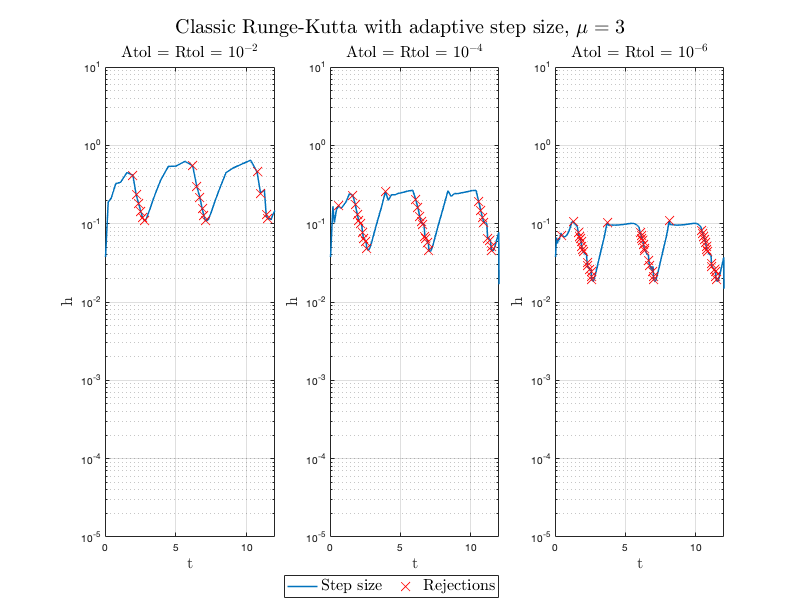
\includegraphics[width=\textwidth]{graphics/opg5/mu3_h.png}
    \caption{Step sizes when solving the Van der Pol with $\mu = 3$ at different tolerances}
    \label{fig5:adap_mu3_h}
\end{figure}

\subsection{Van der Pol, $\mu = 20$}
The Van der Pol problem with $\mu = 20$ is a more complicated problem. The dynamics of the problem is largely defined by the $\mu$ parameter. In particular, the problem becomes more stiff when $\mu$ is increased.

Figure \ref{fig5:fixed_mu20} shows the numerical solution to the Van der Pol problem with $\mu = 20$ for RK4 with $h \in \{0.1, 0.01, 0.001\}$, ODE45 and ODE15s. Notice that there is no visible difference between the solution obtained by ODE45 and ODE15s. For $h=0.1$ the solution once again diverged (as the explicit Euler did). This demonstrated the unfortunate weak property of explicit methods in general. Explicit methods generally have much worse convergence properties compared to implicit methods. In chapter 1 we also showed that RK4 is neither A- nor L-stable, and has a region of stability fairly similar to that of the explicit Euler method. However, when RK4 is within its region of stability, the results are quite good. For both $h=0.01$ and $h=0.001$ there are no visible difference between RK4 and ODE45/ODE15s. 

\begin{figure}[H]
    \centering
    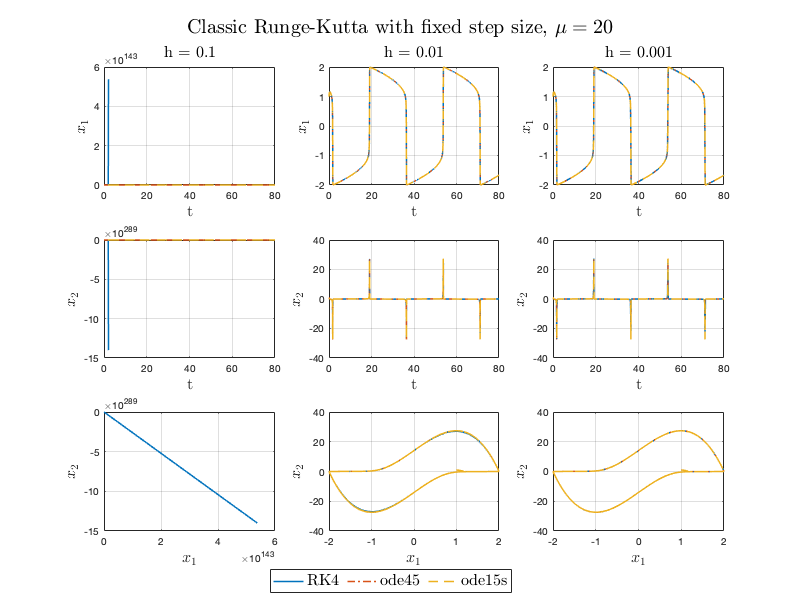
\includegraphics[width=\textwidth]{graphics/opg5/mu20_fixed.png}
    \caption{Solution to Van der Pol with $\mu = 20$ using fixed step sizes}
    \label{fig5:fixed_mu20}
\end{figure}

Table \ref{tab5:mu20_fixed} shows that CPU time and number of function evaluations when solving the Van der Pol problem with $\mu = 20$ using different time steps and Matlab ODE solvers. Notice that with $h=0.1$ the RK4 is faster than any of the other methods, however, as seen above the results are also completely wrong. At a time step of $h=0.01$ RK4 is already slower than ODE45/ODE15s and use many more function calls. At this point there is also no visible difference the results. 

Notice that ODE45 does not outperform ODE15s anymore. This is a good indication that the problem is stiff, i.e., it is worth while to use an implicit method that even when it comes with additional computational cost. The implicit method is also able to use far less function evaluations than the DoPri54. 

\begin{table}[H]
    \centering
    \caption{CPU time and function evaluations of RK4 with fixed time step and Matlab ODE solvers}
    \begin{tabular}{|c||c|c|c|c|c|c|} \hline
         \textbf{Method}    & $h=0.1$&   $h=0.01$ & $h=0.001$ & ODE45 & ODE15s     \\ \hline \hline 
         \textbf{Time}      & 0.0179   & 0.1187  &  1.0235 & 0.0370 & 0.0504   \\ \hline
         \textbf{Fun evals} & 3200    &   32000   &   320000 & 8461 & 926  \\ \hline
    \end{tabular}
    \label{tab5:mu20_fixed}
\end{table}



Figure \ref{fig5:adap_mu20} shows the numerical solution to the Van der Pol problem with $\mu = 20$ for the classical Runge Kutta method with adaptive time steps and $AbsTol=RelTol \in \{10^{-2}, 10^{-4}, 10^{-6}\}$, ODE45 and ODE15s. Notice also that for $Tol = 10^{-2}$ the only difference visible is again due to the relatively large steps that the algorithm takes in the "non-stiff" area. Otherwise, all tolerances seem to follow the ODE45/ODE15s solutions very well.

\begin{figure}[H]
    \centering
    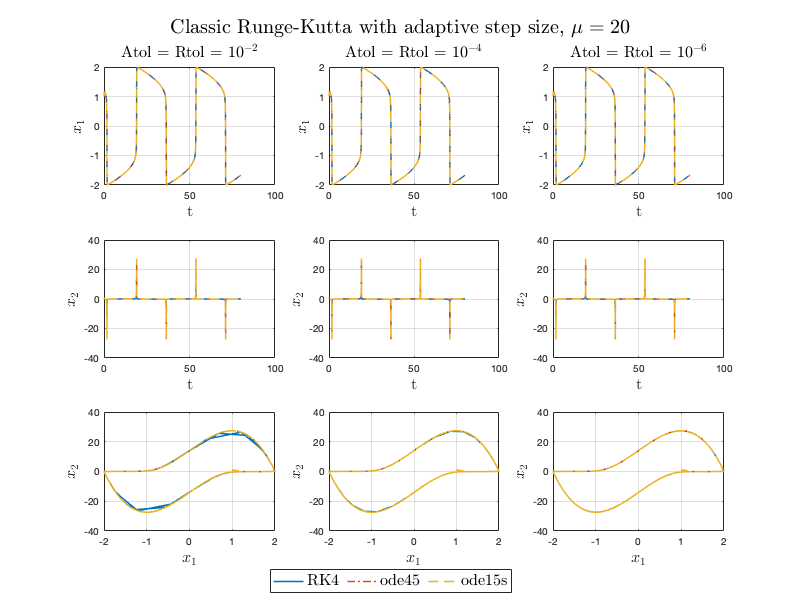
\includegraphics[width=\textwidth]{graphics/opg5/mu20_adap.png}
    \caption{Solution to Van der Pol with $\mu = 20$ using adaptive step sizes}
    \label{fig5:adap_mu20}
\end{figure}

Table \ref{tab5:mu20_adap} shows that CPU time and number of function evaluations when solving the Van der Pol problem with $\mu = 20$ using different tolerances and Matlab ODE solvers. Notice that with $Tol = 10^{-2}$ the RK4 is very similar in speed and number of function calls to ODE45 (and faster then ODE15s). Once again notice that 100 times the accuracy does not require 100 times the CPU time or 100 times the function calls. This is because RK4 is a 4th order method, i.e., the accuracy increase much faster than linear. 

\begin{table}[H]
    \centering
    \caption{CPU time and function evaluations of RK4 with adaptive time step and Matlab ODE solvers}
    \begin{tabular}{|c||c|c|c|c|c|c|} \hline
         \textbf{Method}    & $Tol = 10^{-2}$&   $Tol = 10^{-4}$ & $Tol = 10^{-6}$ & ODE45 & ODE15s     \\ \hline \hline 
         \textbf{Time}      & 0.0365  &  0.2100  &  0.2309 & 0.0386 & 0.0612   \\ \hline
         \textbf{Fun evals} &  9194    &   11306   &    18626 & 8461 & 2944  \\ \hline
    \end{tabular}
    \label{tab5:mu20_adap}
\end{table}

Figure \ref{fig5:adap_mu20_h} shows the used step sizes for the different tolerances. The red crosses mark whenever the step size controller failed to set the step size correctly, i.e., whenever the estimated (using step doubling) error was larger than the allowed maximum. Notice that the behaviour of all three tolerances are quite similar. Also notice that the step sizes does not vary nearly as much for the individual tolerances as previously seen (for explicit- and implicit Euler). Additionally, if we look at the difference in step sizes for the different tolerances, we see that in order to decrease the tolerance by a factor $10^4$, we only need to decrease the step size by a factor $10^1$. This is the true power of higher order methods! And shows that the RK4 is indeed of order 4. 

Finally, notice that the estimated step sizes are quite often rejected, i.e., the step size controller underestimated the need for more accuracy. Judging by the number of rejection for this fairly stiff problem, it might be worthwhile to consider other controller, e.g. a PID controller instead of the asymptotic step size controller we are currently using. 

\begin{figure}[H]
    \centering
    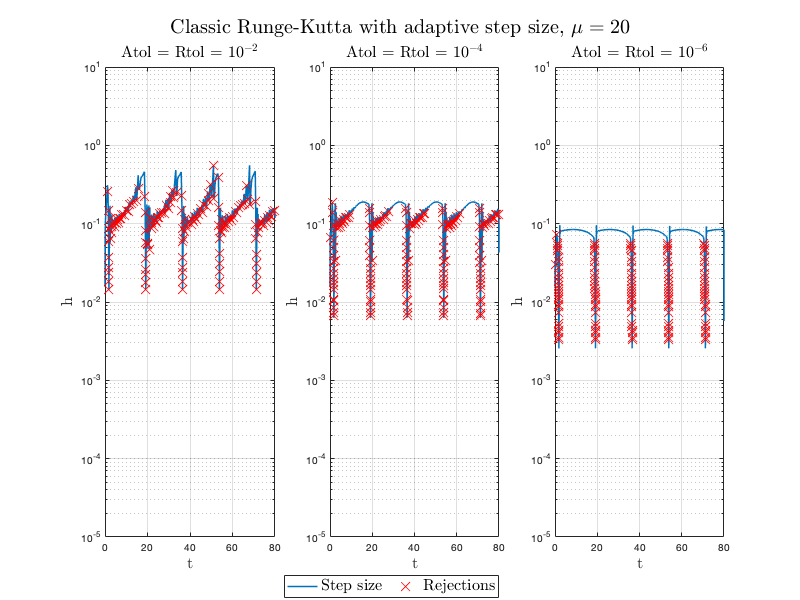
\includegraphics[width=\textwidth]{graphics/opg5/mu20_h.png}
    \caption{Step sizes when solving the Van der Pol with $\mu = 20$ at different tolerances}
    \label{fig5:adap_mu20_h}
\end{figure}






\clearforchapter
\chapter{Dormand-Prince 5(4)}
In the following, we consider the initial value problem (IVP) on the form
\begin{align}
    \dot{x}(t) &= f(t,x(t),p), & x(t_0) = x_0,
\end{align}
where $x \in \probR ^{n_x}$ and $p \in \probR ^{n_p}$. 

\section{Description of Dormand-Prince 5(4)}
The Dorman-Prince 5(4) (DoPri54) method is to a large extend inspired by the classical Runge-Kutta, RK4, outlined in the previous chapter. They are both explicit Runge-Kutta methods, and as such are neither A- nor L-stable regarding the test equation. In practise, DoPri54 is one of the most used methods for solving IVPs on the form given above. In Matlab, it is the method used in the function \textit{ode45}. 

For typical Runge-Kutta methods, we can estimate the errors of the steps by means of step doubling. However, instead of using step doubling to estimate the errors, we can instead use an \textit{embedded} error estimate. Consider the butcher tableau given below

\begin{align}
    \begin{array}{c|cccc}
         c_1 & & & &   \\
         c_2 & a_{21} & & & \\
         \vdots & \vdots  & \vdots & & \\
         c_s & a_{s1} & a_{s2} & \cdots & \\ \hline 
         x & b_1 & b_2 & \cdots & b_s \\
         \hat{x} & \hat b_1 &  \hat b_2 & \cdots & \hat b_s \\ \hline
         e & d_1 & d_2 & \cdots & d_s
    \end{array}
\end{align}

as with RK4 we have 

\begin{align}
    T_i &= t+c_i \cdot h, \quad i = \{1,2,...,s\}\\
    X_i &= x_n + h \cdot \sum_{j=i}^{i-1} a_{ij} f(T_j, X_j), \quad i = \{1,2,...,s\}, \ and \\
    x_{n+1} &= x_n + h \cdot \sum_{i=1}^s b_i f(T_i,X_i).
\end{align}

Now we additionally have 

\begin{align}
    \hat x_{n+1} &= x_n + h \cdot \sum_{i=1}^s \hat b_i f(T_i,X_i) \\
    e_{n+1} &= x_{n+1} - \hat x_{n+1} = h \cdot \sum_{i=1}^s d_i f(T_i,X_i)
\end{align}
where $x_n=x(t_n)$, and $e_n = e(t_n)$. Now we will by design have an error estimate, $e(t)$. The accuracy of the estimate naturally depends on the specific tableau. The reason for using a method with an embedded error estimate is to avoid having to solve multiple steps. Computers are very good at solving linear algebra and as such it can give a computational advantage to use embedded errors estimates compared to step doubling. 

Dormand-Prince 5(4) is a 5th order, 7 stage Runge-Kutta method with embedded error estimation of 4th order. The specific butcher tableau is given by 

\begin{align}
        \begin{array}{c|ccccccc}
0	&0 &&&&&& \\
\frac{1}{5}	&\frac{1}{5} &&&&&& \\
\frac{3}{10}	&\frac{3}{40}	&\frac{9}{40} &&&&& \\
\frac{4}{5}	&\frac{44}{45}	&-\frac{56}{15}	&\frac{32}{9} &&&& \\
\frac{8}{9}	& \frac{19372}{6561}	&-\frac{25360}{2187}	& \frac{64448}{6561}	&-\frac{212}{729} &&& \\
1	&\frac{9017}{3168}	&-\frac{355}{33}	&\frac{46732}{5247}	&\frac{49}{176}	&-\frac{5103}{18656} && \\
1	&\frac{35}{384}	&0	&\frac{500}{1113}	&\frac{125}{192}	&-\frac{2187}{6784}	&\frac{11}{84}	& \\ \hline
x& \frac{35}{384}	&0	&\frac{500}{1113}	&\frac{125}{192}	&-\frac{2187}{6784}	&\frac{11}{84}	&0 \\
\hat{x}&\frac{5179}{57600}	&0	&\frac{7571}{16695}	&\frac{393}{640}	&-\frac{92097}{339200}	&\frac{187}{2100}	&\frac{1}{40} \\ \hline
e & \frac{71}{57600} &0 & -\frac{71}{16695} &\frac{71}{1920} &-\frac{17253}{339200} & \frac{22}{525} &-\frac{1}{40}
    \end{array}
\end{align}

We are now able to define how to select the best step size, $h$. We do so by the \textit{asymptotic step size controller}, this means that our step size is given by
\begin{align}
    h_{k+1} &= \left(\frac{\varepsilon}{r_{k+1}} \right )^{1/6} h_k.
\end{align}
Where $r_{k+1}$ is found by
\begin{align}
    r_{k+1} &= \max_{i \in \{1,...,n_x\}} \left \{ \frac{|e_{k+1}|_i}{ \max \{ |\text{abstol}|_i, \ |x_{k+1}|_i \cdot |\text{reltol}|_i \} } \right \}
\end{align}
where $|\text{abstol}|_i$ and $|\text{reltol}|_i$ are the absolute and relative tolerance of $(x_{k+1})_i$ respectively.

\section{Implementation of Dormand-Prince 5(4)}
Listing \ref{lst6:DoPri54} shows a Matlab implementation of a general explicit Runge-Kutta method with embedded error estimates. The specific parameters that correspond to DoPri54 are listed below the function. 

In the code we see that lines 2-12 initializes parameters, lines 15-17 determines if the an algorithm sould be run to estimate the best initial step size. Line 20 the main loop is initiated, $x_n$, $\hat x_n$, $e_n$ and $r_n$ are estimated. If $r_n \leq 1$ (line 35) we take one step, else we do not. Then the step size, $h$, is estimated (line 43), and if we did take a step, the new values are stored.

\begin{lstlisting}[language=Matlab,caption=Implementation of explicit Runge-Kutta solver with adaptive time step using embedded error estimates. Parameters corresponding to DoPri54 given at the end,label=lst6:DoPri54]
function [x,t,function_calls,hs] = explicitRungeKuttaEmbedded(f,param,h,t0,T,x0,A,b,bhat,c,Atol,Rtol,hmin,hmax,eps_tol,p,initial_step_algo)
    N = ceil((T-t0)/hmin);
    s = length(b);
    d = length(x0);
    t = zeros(1,N+1);
    hs = zeros(1,N+1);
    x = zeros(length(x0),N+1);
    k = zeros(d,s)';
    t(1) = t0;
    x(:,1) = x0;
    accept_step = false;
    function_calls = 0;
    
    
    if initial_step_algo % slide 4b, 9 whic is from p169 Hairer
        [h,function_calls] = initialStepSize(f,param,t0,x0);
    end
    
    i = 2;
    while t(i-1)<=T
        
       while(~accept_step)
           k = 0*k;
           for j = 1:s
               k(j,:) = f(t(i-1)+h*c(j),x(:,i-1)+sum(h*k.*A(j,:)',1)', param);
               function_calls = function_calls +1;
           end
           oneAhead = x(:,i-1)+sum(h*k.*b,1)';
           oneAheadhat = x(:,i-1)+sum(h*k.*bhat,1)';
           
           % Embedded error estimate
           e = abs(oneAhead-oneAheadhat);
           r = max(e./max(Atol,abs(oneAhead).*Rtol));
           
           if r<=1
               x(:,i) = oneAhead;
               hs(i-1) = h;
               t(i) = t(i-1)+h;
               accept_step = true;
           else
               accept_step = false;
           end
           h = h*max(hmin,min(hmax,(eps_tol/r)^(1/(1+p)))); % eq 4.13 in Harier
           
       end
       accept_step = false;
       i = i+1;
    end
    x = x(:,1:i-1)';
    t = t(1:i-1);
    hs = hs(1:i-2);
end

%% DoPri54 parameters
c = [0 1/5 3/10 4/5 8/9 1 1]';
A = [0 0 0 0 0 0 0 ;
     1/5 0 0 0 0 0 0
     3/40 9/40 0 0 0 0 0 ;
     44/45 -56/15 32/9 0 0 0 0 ;
     19372/6561 -25360/2187 64448/6561 -212/729 0 0 0;
     9017/3168 -355/33 46732/5247 49/176 -5103/18656 0 0;
     35/384 0 500/1113 125/192 -2187/6784 11/84 0];
b = [35/384 0 500/1113 125/192 -2187/6784 11/84 0]';
bhat = [5179/57600 0 7571/16695 393/640 -92097/339200 187/2100 1/40]';
p = 5;
\end{lstlisting}

\section{Test on the test equation}
As previously mentioned, \textit{stability}, i.e., how the methods converge, of numerical methods are an important characteristic of any numerical method. We have introduced the test equation in chapter 1, and we will use this to say something about the stability of numerical methods. It is important to remember that stability is seen in this exact context, i.e., how the method perform on the test equation with a given set of parameters. 

Again, we define the stability function, $R(\mu)$, by the relation

\begin{align}
    x(t+h) &= R(\mu) x(t).
\end{align}

Now, cf Ascher\cite{Ascher} (alternatively slide 8B), we know that for Runge Kutta methods we have

\begin{align}
    R(\mu) &= 1 + \mu b^T (I-\mu A)^{-1} e.
\end{align}

Then
\begin{align}
    e_{n+1} &= x_{n+1} - x(t_{n+1}) = \left [ R(\mu) - exp(\mu) \right] x_n.
\end{align}

The stability function now simplifies to 

\begin{align}
    R(\mu) &= 1 + \mu + \frac{\mu^2}{2} + \frac{\mu^3}{6} + \frac{\mu^4}{24} + \frac{\mu^5}{120} + \frac{\mu^6}{600}.
\end{align}

We remember that the stability region is given by

\begin{align}
    \mathcal{S} = \left \{ \mu \in \mathcal{C} \ | \ |R(\mu)| \leq 1 \right \}.
\end{align}

Figure \ref{fig6:dopri_stability} shows the stability region of the Dormand-Prince 5(4) method. As previously stated, the method is neither A- nor L-stable. 

\begin{figure}[H]
    \centering
    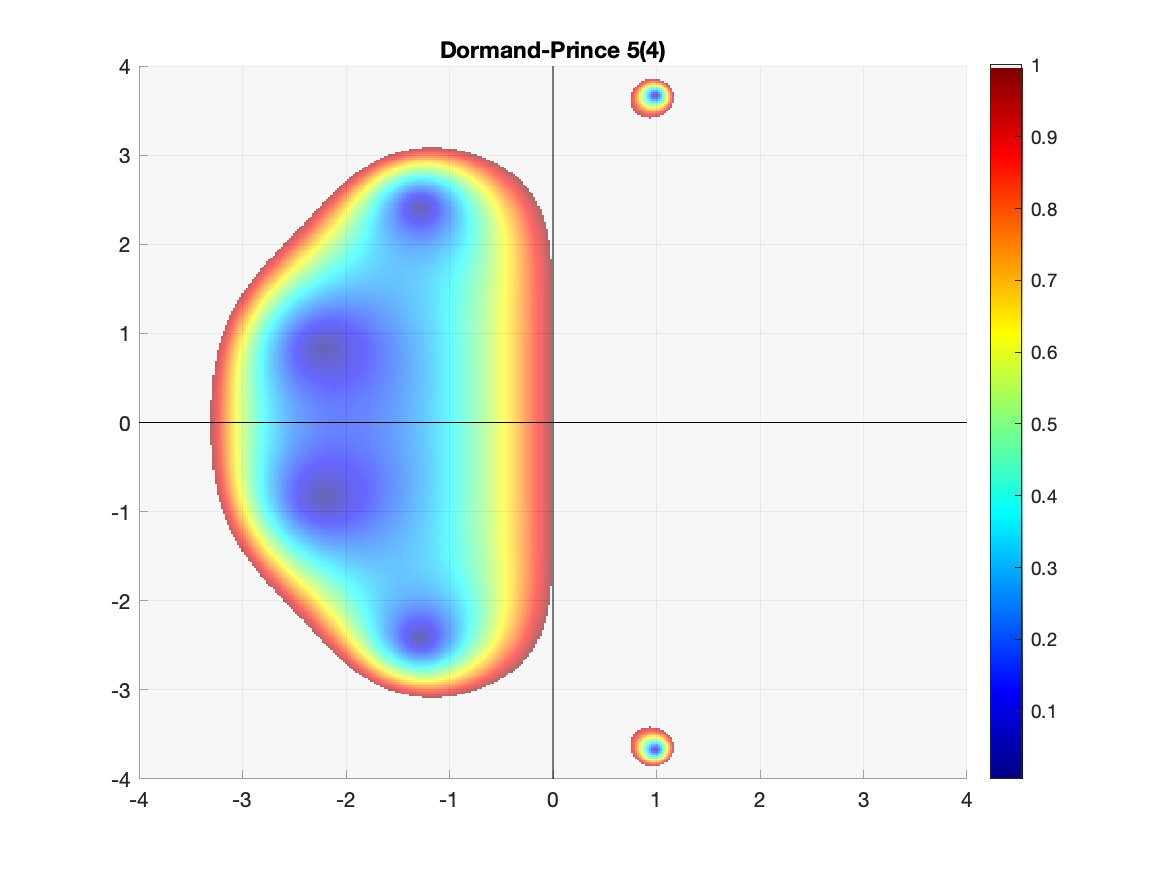
\includegraphics[width=10cm]{graphics/opg6/dopri-stability.png}
    \caption{Stability region of Dormand-Prince 5(4) method on test equation. The colored region is the stable region.}
    \label{fig6:dopri_stability}
\end{figure}


Regarding the order of the DoPri54, it is tedious to show a full proof of the order, as it required knowledge about \textit{rooted trees} and Hopf algebra. However, in Ascher\cite{Ascher} it is shown that DoPri54 has order 5, and the error estimate has order 4. 

Figure \ref{fig6:test_problem} shows the solution, local truncation error and global truncation error for the test problem with a fixed step size of $h=1$. Additionally, it also shows the analytical errors, i.e., the errors we expect DoPri54 to make with this step size. Notice how the dots are the discrete realizations of the analytical curves. 

\begin{figure}[H]
    \centering
    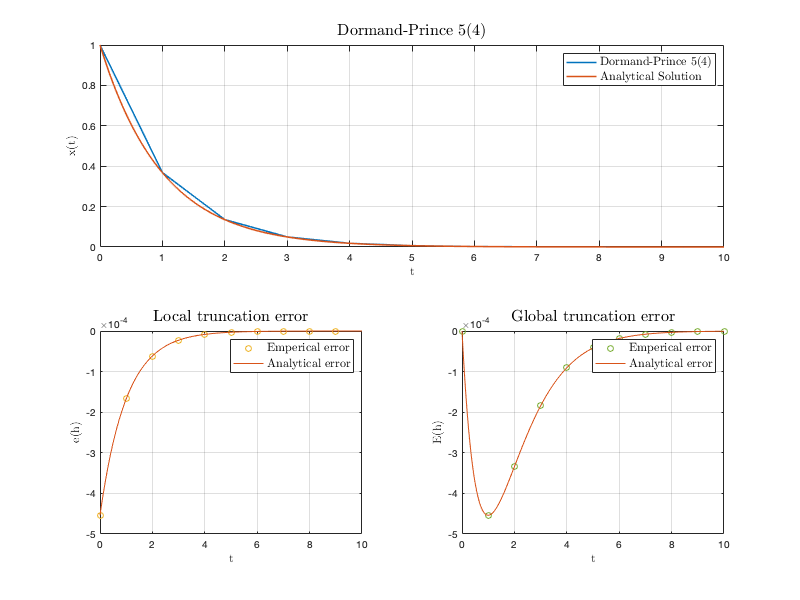
\includegraphics[width=10cm]{graphics/opg6/test_problem.png}
    \caption{Solution, local truncation error and global truncation error for the test problem}
    \label{fig6:test_problem}
\end{figure}



\section{Test on Van der Pol problem and comparison with Matlab ODE solvers}
Now that we have made an implementation of DoPri54 with adaptive step size we want to test it. To do so we look at the Van der Pol problem given by
\begin{align}
    \Ddot{x}(t) &= \mu (1-x(t)^2) \dot{x}(t) - x(t).
\end{align}
To solve the problem we must first re-write the problem as a system of first order differential equations. Luckily this is done easily and given by
\begin{align}
    \dot{x}_1(t) &= x_2(t) \\
    \dot{x}_2(t) &= \mu(1-x_1(t)^2) x_2(t) - x_1(t).
\end{align}

We will now test DoPri54 on the Van der Pol problem with $\mu = 3$ and $\mu = 20$. 

\subsection{Van der Pol, $\mu = 3$}
Figure \ref{fig6:adap_mu3} shows the numerical solution to the Van der Pol problem with $\mu = 3$ for DoPri54 with adaptive time steps and $AbsTol=RelTol \in \{10^{-2}, 10^{-4}, 10^{-6}\}$, ODE45 and ODE15s. Notice also that for $Tol = 10^{-2}$ we see some difference in the plots. It is simply because at the tolerance, DoPri54 take such large time steps, that we can see the straight lines by Matlab. This is especially visible in the "corner" of the solution curve.

\begin{figure}[H]
    \centering
    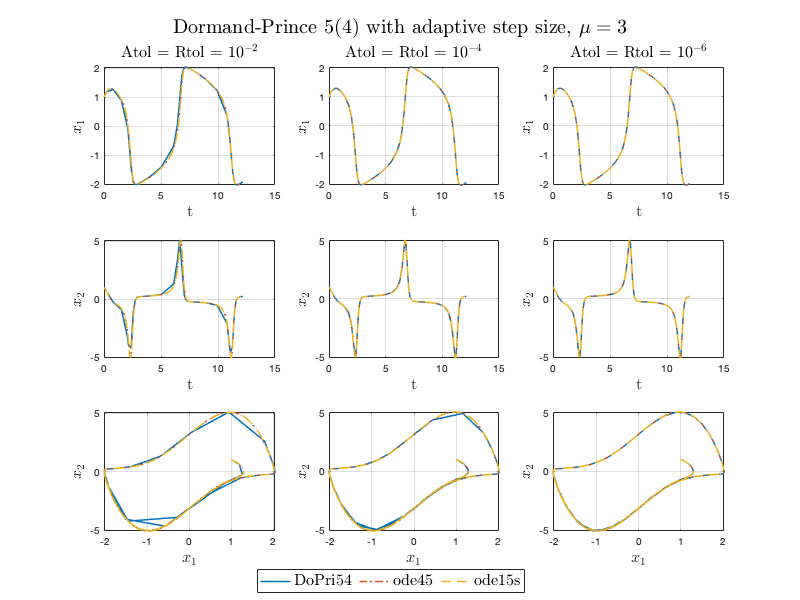
\includegraphics[width=\textwidth]{graphics/opg6/mu3_adap.png}
    \caption{Solution to Van der Pol with $\mu = 3$ using adaptive step sizes}
    \label{fig6:adap_mu3}
\end{figure}

Table \ref{tab6:mu3_adap} shows the CPU time and number of function evaluations when solving the Van der Pol problem with $\mu = 3$ using different tolerances and Matlab ODE solvers. Notice that with $Tol = 10^{-2}$ the DoPri54 is relatively fast (slower than ODE45 but faster than ODE15s). Generally, it is very hard to tell the solutions curves apart just by looking at them. Even for the lowest tolerance, we get quite good results. What is interesting is the CPU time usage and number of function evaluations used at the different tolerances. For both explicit- and implicit Euler, we saw that the CPU time and function evaluations increased dramatically when we required higher accuracy, now this increase is not as pronounced. This demonstrates the power of higher order methods quite well.

One of the reasons why ODE45 is able to outperform the DoPri45 with adaptive step size is because it has lower overhead. ODE45 uses the same algorithm as DoPri45, so we would expect the same asymptotic performance. Additionally, ODE45 might employ a different step size controller---this will obviously also affect the performance. 

\begin{table}[H]
    \centering
    \caption{CPU time and function evaluations of DoPri54 with adaptive time step and Matlab ODE solvers}
    \begin{tabular}{|c||c|c|c|c|c|c|} \hline
         \textbf{Method}    & $Tol = 10^{-2}$&   $Tol = 10^{-4}$ & $Tol = 10^{-6}$ & ODE45 & ODE15s     \\ \hline \hline 
         \textbf{Time}      & 0.0059  &  0.0376  &  0.0160 & 0.0046 & 0.0175   \\ \hline
         \textbf{Fun evals} & 373     &    681   &     1332 & 1069 & 926  \\ \hline
    \end{tabular}
    \label{tab6:mu3_adap}
\end{table}

Figure \ref{fig6:adap_mu3_h} shows the used step sizes for the different tolerances. The red crosses mark whenever the step size controller failed to set the step size correctly, i.e., whenever the estimated (using the embedded error estimate) error was larger than the allowed maximum. Notice that the behaviour of all three tolerances are quite similar. Also notice that the step sizes does not vary nearly as much for the individual tolerances as previously seen (for explicit- and implicit Euler). Additionally, if we look at the difference in step sizes for the different tolerances, we see that in order to decrease the tolerance by a factor $10^4$, we do not even need to decrease the step size by a factor $10^1$. This is the true power of higher order methods! And shows that the DoPri54 is indeed of order 5. 

\begin{figure}[H]
    \centering
    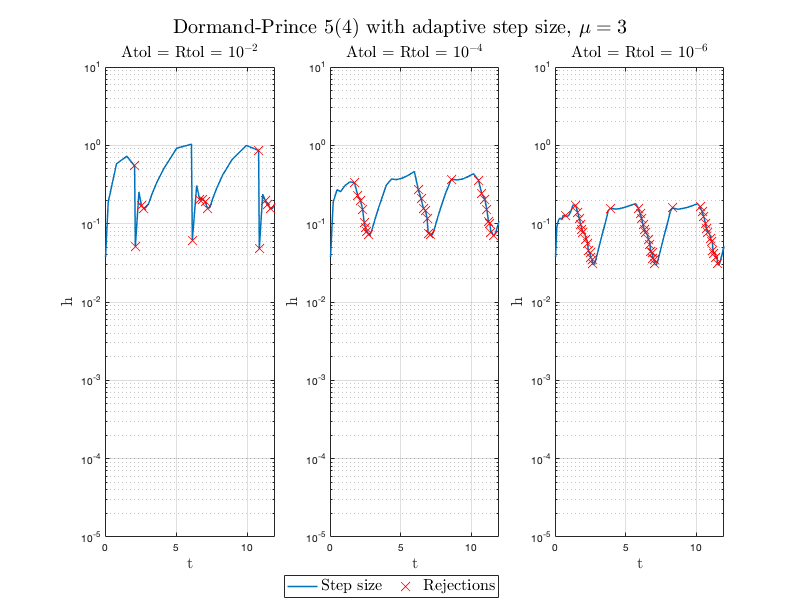
\includegraphics[width=\textwidth]{graphics/opg6/mu3_h.png}
    \caption{Step sizes when solving the Van der Pol with $\mu = 3$ at different tolerances}
    \label{fig6:adap_mu3_h}
\end{figure}

\subsection{Van der Pol, $\mu = 20$}
The Van der Pol problem with $\mu = 20$ is a more complicated problem. The dynamics of the problem is largely defined by the $\mu$ parameter. In particular, the problem becomes more stiff when $\mu$ is increased.

Figure \ref{fig6:adap_mu20} shows the numerical solution to the Van der Pol problem with $\mu = 20$ for DoPri54 with adaptive time steps and $AbsTol=RelTol \in \{10^{-2}, 10^{-4}, 10^{-6}\}$, ODE45 and ODE15s. Notice also that for $Tol = 10^{-2}$ the only difference visible is again due to the relatively large steps that the algorithm takes in the "non-stiff" area. Otherwise, all tolerances seem to follow the ODE45/ODE15s solutions very well.

\begin{figure}[H]
    \centering
    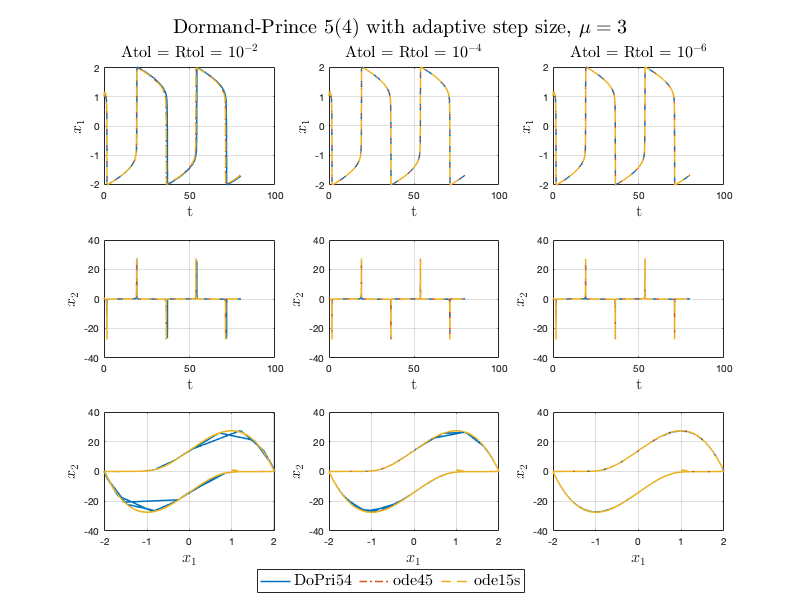
\includegraphics[width=\textwidth]{graphics/opg6/mu20_adap.png}
    \caption{Solution to Van der Pol with $\mu = 20$ using adaptive step sizes}
    \label{fig6:adap_mu20}
\end{figure}

Table \ref{tab6:mu20_adap} shows that CPU time and number of function evaluations when solving the Van der Pol problem with $\mu = 20$ using different tolerances and Matlab ODE solvers. Notice that with $Tol = 10^{-2}$ the DoPri54 is very similar in speed to ODE45 (and faster than ODE15s). Once again notice that 100 times the accuracy does not require 100 times the CPU time or 100 times the function calls. This is because DoPri54 is a 5th order method, i.e., the accuracy increase much faster than linear. Particular notice the relatively low difference in number of function calls between the tolerances.

\begin{table}[H]
    \centering
    \caption{CPU time and function evaluations of DoPri54 with adaptive time step and Matlab ODE solvers}
    \begin{tabular}{|c||c|c|c|c|c|c|} \hline
         \textbf{Method}    & $Tol = 10^{-2}$&   $Tol = 10^{-4}$ & $Tol = 10^{-6}$ & ODE45 & ODE15s     \\ \hline \hline 
         \textbf{Time}      & 0.0344 &   0.1419  &  0.2723 & 0.0386 & 0.0612   \\ \hline
         \textbf{Fun evals} &  6708    &    7422   &     9522 & 8461 & 2944  \\ \hline
    \end{tabular}
    \label{tab6:mu20_adap}
\end{table}

Figure \ref{fig6:adap_mu20_h} shows the used step sizes for the different tolerances. The red crosses mark whenever the step size controller failed to set the step size correctly, i.e., whenever the estimated error was larger than the allowed maximum. Notice that the behaviour of all three tolerances are not nearly as similar as previously seen. This time especially the most accurate tolerance struggles to determine the correct step sizes. This is mainly because the method generally takes very large steps (being a 5th order method), hence the change in step sizes can be very big in stiff areas. Also notice that the step sizes does not vary nearly as much for the individual tolerances as previously seen (for explicit- and implicit Euler). 

Finally, notice that the estimated step sizes are quite often rejected, i.e., the step size controller underestimated the need for more accuracy. Judging by the number of rejection for this fairly stiff problem, it might be worthwhile to consider other controller, e.g. a PID controller instead of the asymptotic step size controller we are currently using. 

\begin{figure}[H]
    \centering
    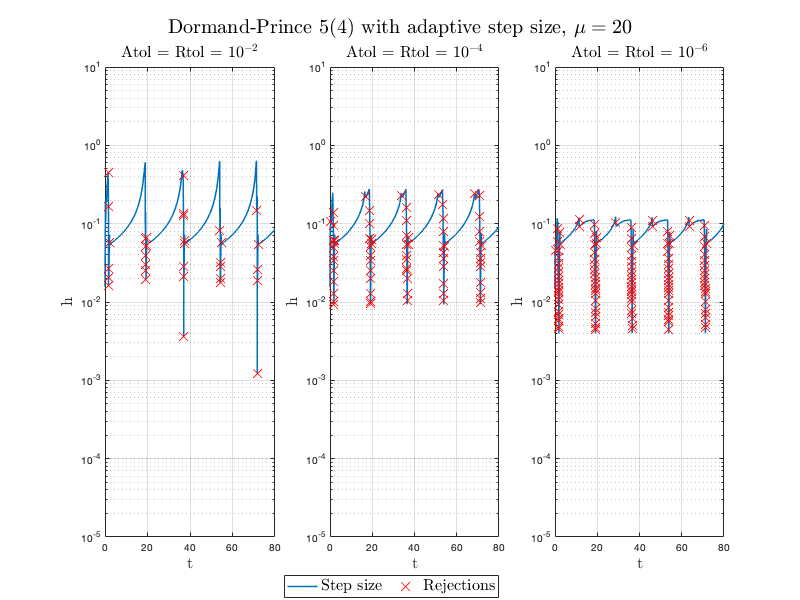
\includegraphics[width=\textwidth]{graphics/opg6/mu20_h.png}
    \caption{Step sizes when solving the Van der Pol with $\mu = 20$ at different tolerances}
    \label{fig6:adap_mu20_h}
\end{figure}


 
\section{Test on CSTR problem and comparison with Matlab ODE solvers}
To furhter test the DoPri54, we will also perform test on the adiabatic continuous stirred tank reactor (CSTR). The process is described in depth in \cite{cstr}, it is essentially a exothermic chemical reaction happening in two connected tanks. We will focus on the temperature of the tanks, and not look to much into the concentration of active compounds. 

The temperature of the CSTR problem is generally modelled by a system of three ODEs (where one is temperature), we will refer to this as the 3D system. However, as shown in the article, the dynamics of the temperature can be approximated by a single ODE, i.e., a 1D system. We will perform analysis of both the 1D and the 3D system.

The 1D CSTR system is given by

\begin{align}
    \dot T &=  \frac{F}{V} (T_{in} − T)+R_T (C_A(T),C_B(T),T)
\end{align}

and the 3D is given by

\begin{align}
\dot{C}_{A} &=\frac{F}{V}\left(C_{A, i n}-C_{A}\right)+R_{A}\left(C_{A}, C_{B}, T\right) \\
\dot{C}_{B} &=\frac{F}{V}\left(C_{B, i n}-C_{B}\right)+R_{B}\left(C_{A}, C_{B}, T\right) \\
\dot{T} &=\frac{F}{V}\left(T_{i n}-T\right)+R_{T}\left(C_{A}, C_{B}, T\right)
\end{align}

where all are constants. There is a small caveat---we will adjust the value of $F$ every 2 minutes. Figure \ref{fig6:f-val} shows the values of $F$ used in the CTSR problems. Notice we assume the value is modulated in 2min intervals. 

\begin{figure}[H]
    \centering
    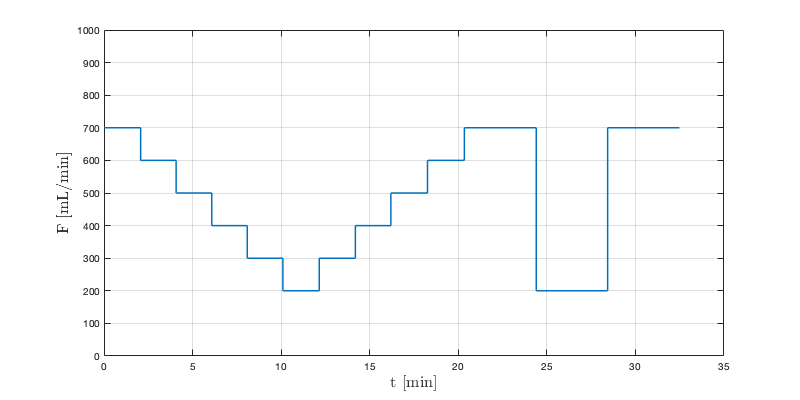
\includegraphics[width=\textwidth]{graphics/opg6/f-val.png}
    \caption{Value of $F$ as a function of time}
    \label{fig6:f-val}
\end{figure}

\subsection{1D}
We are now able to solve the IVP using the $F$ given above and constant parameters as given in \cite{cstr}. Figure \ref{fig6:1d_sol} shows the solution to the 1D CSTR using $AbsTol=RelTol \in \{10^{-2}, 10^{-4}, 10^{-6}\}$, together with solutions using ODE45 and ODE15s. For $Tol=10^{-2}$ we see some deviation from DoPri54 to ODE45/ODE15s, especially in areas where there is a fairly abrupt change in dynamics, i.e., areas that are stiff. For the tolerances $Tol \in \{10^{-4}, 10^{-6}\}$ there is no visible difference between the ODE45/ODE15s and DoPri54.

\begin{figure}[H]
    \centering
    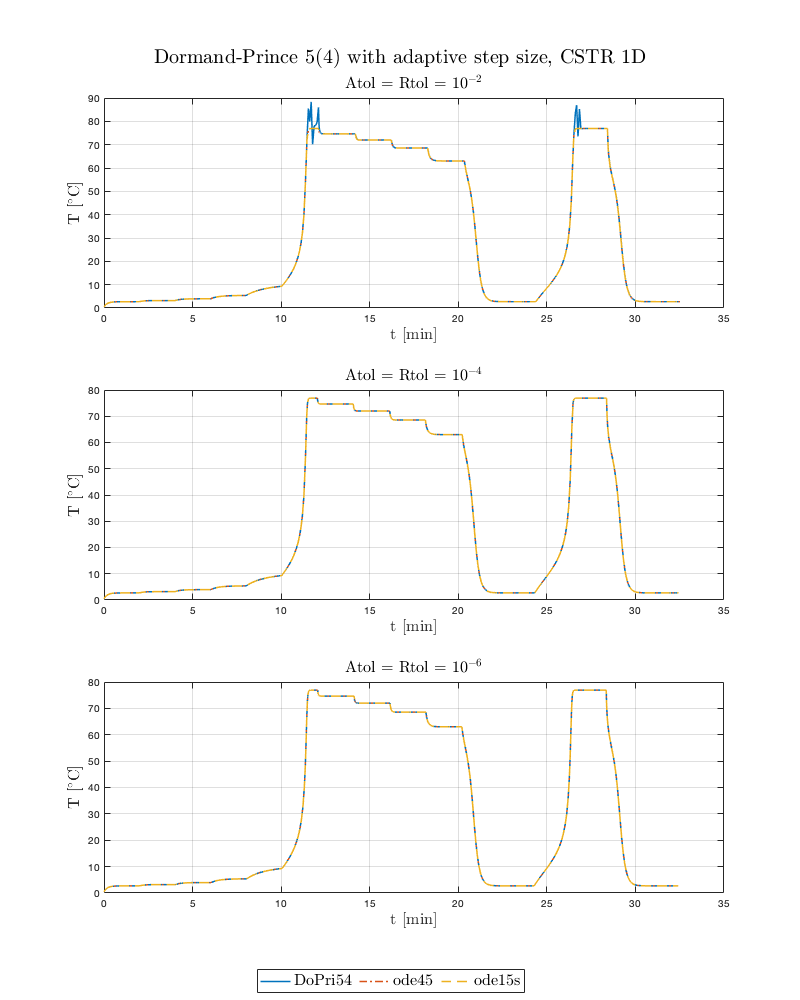
\includegraphics[width=\textwidth]{graphics/opg6/cstr-1d.png}
    \caption{Solutions to 1D CSTR using adaptive time step DoPri54}
    \label{fig6:1d_sol}
\end{figure}

Table \ref{tab6:1d_cstr} shows the CPU time and number of function evaluations for DoPri54 with varying tolerances, ODE45 and ODE15s. Notice that all DoPri45 methods use very similar number of function calls, and in fact they almost use exactly the same time. Notice also that ODE45 and ODE15s outperform DoPri54 quite dramicially, especially considering that they use more function calls. The reason for this is quite simply because ODE45/ODE15s has less overhead, i.e., it is not as expensive to call the function. In this setup, where all functions are call several times, this overhead becomes quite important. 

\begin{table}[H]
    \centering
    \caption{CPU time and function evaluations of DoPri54 with adaptive time step and Matlab ODE solvers}
    \begin{tabular}{|c||c|c|c|c|c|c|} \hline
         \textbf{Method}    & $Tol = 10^{-2}$&   $Tol = 10^{-4}$ & $Tol = 10^{-6}$ & ODE45 & ODE15s     \\ \hline \hline 
         \textbf{Time}      & 0.6190 &   0.5789  &  0.5667 & 0.0413 & 0.0814   \\ \hline
         \textbf{Fun evals} &  2902  &   2986    &  3266   &   5886 & 4308  \\ \hline
    \end{tabular}
    \label{tab6:1d_cstr}
\end{table}

Figure \ref{fig6:1d_h} shows the step sizes when solving the 1D CSTR using DoPri54 with adaptive time steps for the different tolerances. Notice that for the most part, the step sizes for the 3 tolerances are almost the same. This is because the CSTR problem for the most part is quite smooth, i.e., it is easy for good solver to find good solutions. However, there are some areas where the problem changes dynamics quite rapidly. We see this as very sudden drops in step sizes. Notice the difference between the drop at the different tolerances. For the low tolerance the drops are much deeper than for the large tolerance. This is seen as the deviations as discussed above.

\begin{figure}[H]
    \centering
    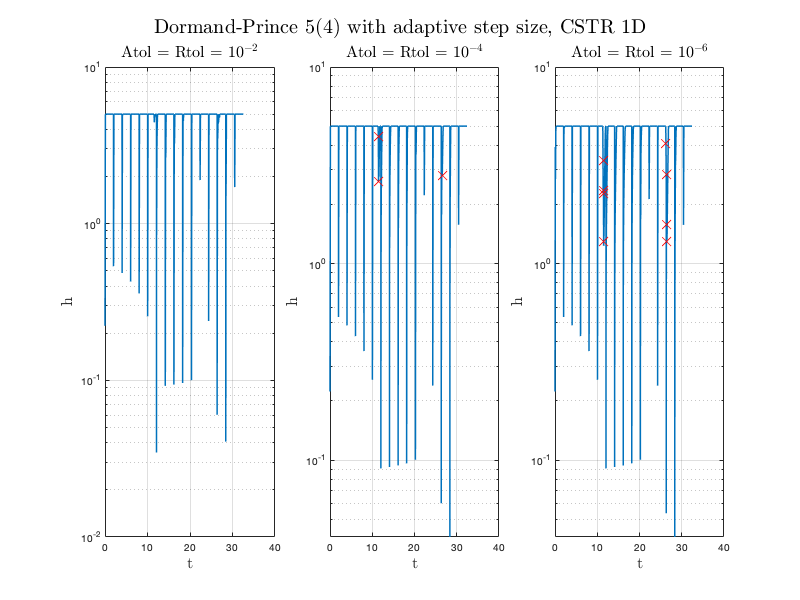
\includegraphics[width=\textwidth]{graphics/opg6/cstr_1d_h.png}
    \caption{Step sizes when solving the 1D CSTR using adaptive time step DoPri54}
    \label{fig6:1d_h}
\end{figure}

\subsection{3D}
Figure \ref{fig6:3d_sol} shows the solution to the 3D CSTR using $AbsTol=RelTol \in \{10^{-2}, 10^{-4}, 10^{-6}\}$, together with solutions using ODE45 and ODE15s. For $Tol=10^{-2}$ we see some deviation from DoPri54 to ODE45/ODE15s. This time the differences do not occur at the corner, but rather just after. For the tolerances $Tol \in \{10^{-4}, 10^{-6}\}$ there is no visible difference between the ODE45/ODE15s and DoPri54.

\begin{figure}[H]
    \centering
    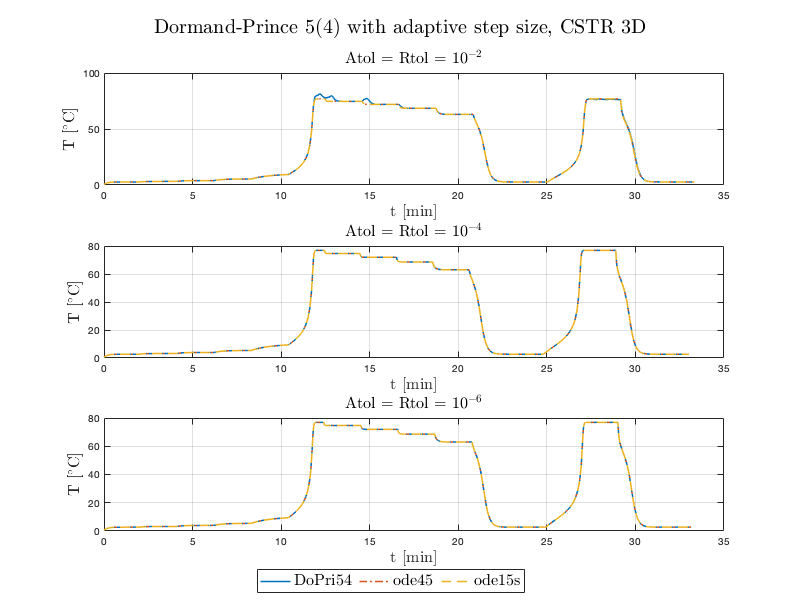
\includegraphics[width=\textwidth]{graphics/opg6/cstr-3d.png}
    \caption{Solutions to 3D CSTR using adaptive time step DoPri54}
    \label{fig6:3d_sol}
\end{figure}

Table \ref{tab6:3d_cstr} shows the CPU time and number of function evaluations for DoPri54 with varying tolerances, ODE45 and ODE15s. Notice that all DoPri45 methods use very similar number of function calls, and in fact they almost use exactly the same time. Notice also that ODE45 outperform DoPri54 quite dramatically, but this time ODE15s does not! For some reason our implementation of DoPri54 is faster for the 3D system than the 1D system. One possible reason for this is that that the 3D system is less stiff than the 1D system, and hence the optimal step size is easier obtained, and step sizes can be larger. Notice in particular the large difference in number of function calls between DoPri54 and ODE45/ODE15s. It seems that our implementation is able to take some really large steps.

\begin{table}[H]
    \centering
    \caption{CPU time and function evaluations of DoPri54 with adaptive time step and Matlab ODE solvers}
    \begin{tabular}{|c||c|c|c|c|c|c|} \hline
         \textbf{Method}    & $Tol = 10^{-2}$&   $Tol = 10^{-4}$ & $Tol = 10^{-6}$ & ODE45 & ODE15s     \\ \hline \hline 
         \textbf{Time}      & 0.2747 &   0.2420  &   0.2460 & 0.0899 & 0.6997   \\ \hline
         \textbf{Fun evals} &  1743     &   1477    &    2289   &  24828 & 15603  \\ \hline
    \end{tabular}
    \label{tab6:3d_cstr}
\end{table}

Figure \ref{fig6:3d_h} shows the step sizes when solving the 3D CSTR using DoPri54 with adaptive time steps for the different tolerances. Notice that for the most part, the step sizes for the 3 tolerances are almost the same. This is because the CSTR problem for the most part is quite smooth, i.e., it is easy for good solver to find good solutions. However, there are some areas where the problem changes dynamics quite rapidly. We see this as very sudden drops in step sizes. Notice the difference between the drop at the different tolerances. For the high tolerance the drops are much deeper than for the low tolerance. It seems that the asymptotic step size controller expects the most sudden change for the large tolerance. This might be the reason why the large tolerance is slower than the lower tolerances. Also notice that the step sizes are really large for some parts, with step sizes well above 10s! Finally, notice how much smoother this plot is compared to the 1D version. This really underlines that while the 1D version might be of lower dimension, that does not necessarily make it an easier problem. 

\begin{figure}[H]
    \centering
    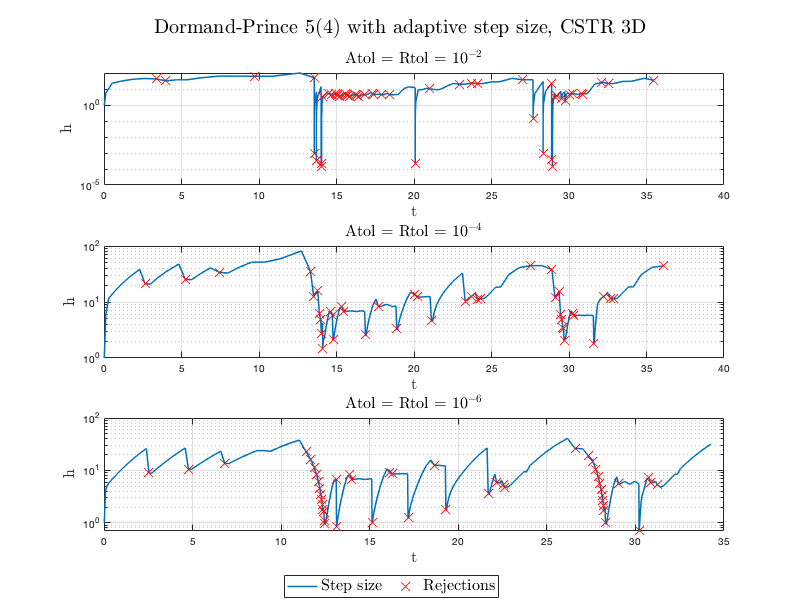
\includegraphics[width=\textwidth]{graphics/opg6/cstr_3d_h.png}
    \caption{Step sizes when solving the 3D CSTR using adaptive time step DoPri54}
    \label{fig6:3d_h}
\end{figure}







\clearforchapter
\chapter{ESDIRK23}
In the following, we consider the initial value problem (IVP) on the form
\begin{align}
    \dot{x}(t) &= f(t,x(t),p), & x(t_0) = x_0,
\end{align}
where $x \in \probR ^{n_x}$ and $p \in \probR ^{n_p}$. 

\section{Description of ESDIRK23}
In this final chapter, we consider a special type of implicit Runge-Kutta methods, namely the explicit singly diagonal implicit Runge-Kutta (ESDIRK) integration methods. These are generally used for systems of stiff differential equations. Remember that any s-stage Runge-Kutta methods with embedded error estimates follow 

\begin{align}
    T_i &= t_n+c_i \cdot h, \quad i = \{1,2,...,s\}\\
    X_i &= x_n + h \cdot \sum_{j=i}^{i-1} a_{ij} f(T_j, X_j), \quad i = \{2,3,...,s\}, \ and \\
    x_{n+1} &= x_n + h \cdot \sum_{i=1}^s b_i f(T_i,X_i) \\
    \hat x_{n+1} &= x_n + h \cdot \sum_{i=1}^s \hat b_i f(T_i,X_i) \\
    e_{n+1} &= x_{n+1} - \hat x_{n+1} = h \cdot \sum_{i=1}^s d_i f(T_i,X_i)
\end{align}
where $x_{n} = x(t_n)$, $\hat{x}_n = \hat x(t_n)$ and $e_n = e(t_n)$. 

The class of Runge-Kutta methods is very diverse and there big difference between the various implementations. All classes, however, are described by their \textit{butcher tableau}. This butcher tableau is given on the form (for RK methods with embedded error estimates)

\begin{align}
    \begin{array}{c|c}
        c & A  \\ \hline
        x & b  \\
        \hat{x} & \hat{b} \\ \hline
        e & d
    \end{array}
\end{align}

From the A matrix it is possible to see whether a method is explicit or implicit. Iff A is a lower triangular matrix, then the method is explicit. Fully implicits methods are generally great at dealing with stiff systems, but they come at a great computational cost. Therefore, diagonally implicit Runge-Kutta (DIRK), singly diagonally implicit Runge-Kutta (SDIRK), and explicit singly diagonally implicit Runge-Kutta (ESDIRK) methods were invented. They have some of the good stability properties of fully implicit methods, but at a lower cost. 

We will focus on the ESDIRK methods, i.e., Runge-Kutta methods whose butcher tableau is given on the form

\begin{align}
    \begin{array}{l|l|lllll}
0 & 0 & 0 & 0 & \ldots & 0 & 0 \\
\hline c_{2} & a_{21} & \gamma & 0 & \ldots & 0 & 0 \\
c_{3} & a_{31} & a_{32} & \gamma & \ldots & 0 & 0 \\
\vdots & \vdots & \vdots & \vdots & & \vdots & \vdots \\
c_{s-1} & a_{s-1,1} & a_{s-1,2} & a_{s-1,3} & \ldots & \gamma & 0 \\
1 & b_{1} & b_{2} & b_{3} & \ldots & b_{s-1} & \gamma \\
\hline & b_{1} & b_{2} & b_{3} & \ldots & b_{s-1} & \gamma
\end{array}
\end{align}

Specifically, we will look at the 3-stage ESDIRK23 given by

\begin{align}
    \begin{array}{c|ccc}
0 & 0 & & \\
c_{2} & a_{21} & \gamma & \\
1 & b_{1} & b_{2} & \gamma \\
\hline x_{n+1} & b_{1} & b_{2} & \gamma \\
\hat{x}_{n+1} & \hat{b}_{1} & \hat{b}_{2} & \hat{b}_{3} \\
\hline e_{n+1} & d_{1} & d_{2} & d_{3}
\end{array}
\end{align}

For ESDIRK23 the first step is explicit since $c_1 = 0$ and $a_{11} = 0$. Stages $\{2, .., s\}$ are singly diagonally implicit. From the butcher table, we can see that the last $X_i$ is equal to $x(t+h)$, which reduce compute time. It also makes it stiffly accurate. Stiffly accurate
methods avoid the order reduction for stiff systems. Further $\hat x(t)$ is of order 3, as shown by Jørgensen\cite{dotdot2018}. They also showed that the stability function in a 3 stage, stiffly accurate ESDIRK method is given by

\begin{align}
    R(z)=\frac{1+\left(b_{1}+b_{2}-\gamma\right) z+\left(a_{21} b_{2}-b_{1} \gamma\right) z^{2}}{(1-\gamma z)^{2}}.
\end{align}

In order to be L-stable, the numerator order must be less than the denominator order in in the stability function, so

\begin{align}
    a_{21} b_{2}-b_{1} \gamma = 0
\end{align}
Additionally, the consistency requirements must be satisfied 

\begin{align}
    \sum_{j=1}^s a_{ij} c_j = \frac{1}{2}c_i^2, \quad i \in \{2,...,s-1\} \quad \Rightarrow \\
    c_2 = a_{21} + \gamma \\
    1 = b_1 + b_2 + \gamma 
\end{align}

Finally, the order conditions are given by

\begin{align}
    Order \ 1: \quad & b_1 + b_2 + \gamma = 1 \\
    Order \ 2: \quad & b_2 c_2 + \gamma = \frac{1}{2} \\
    Order \ 3: \quad & b_2 c_2^2 + \gamma = \frac{1}{3}.
\end{align}

We can now solve the system and find parameters such that the system is of order 3. Unfortunately, upon revision, we see that there exists no solution of order 3 that are also L-stable! In stead, we settle for a solution of order 2, here a L-stable solutions does exit. We get

\begin{align}
    b_1 = b_2 = \frac{1- \gamma}{2} \\
    c_2 = 2 \gamma \\
    \gamma = \frac{2- \sqrt{2}}{2}.
\end{align}

Similarly, we can find the $\hat b's$, such that $\hat x$ satisfies the 3. order conditions. In the end, we get the L-stable stiffly accurate 2. order method with an embedded 3. order error estimate summarized by the butcher tableau 

\begin{align}
    \begin{array}{c|ccc}
0 & 0 & & \\
2 \gamma & \gamma & \gamma & \gamma \\
1 & \frac{1-\gamma}{2} & \frac{1-\gamma}{2} & \gamma \\
\hline x_{n+1} & \frac{1-\gamma}{2} & \frac{1-\gamma}{2} & \frac{1-3 \gamma}{3(1-2 \gamma)} \\
\hat{x}_{n+1} & \frac{6 \gamma-1}{12 \gamma} & \frac{1}{12 \gamma(1-2 \gamma)} & \frac{6 \gamma(1-\gamma)-1}{3(1-2 \gamma)}
\end{array}
\end{align}

where $\gamma = \frac{2- \sqrt{2}}{2}$. This is known as ESDIRK23. 

\section{Stability of ESDIRK23}
Let us remember that the stability function for any stiff accurate ESDIRK method is given by\cite{dotdot2018} 

\begin{align}
    R(z)=\frac{1+\left(b_{1}+b_{2}-\gamma\right) z+\left(a_{21} b_{2}-b_{1} \gamma\right) z^{2}}{(1-\gamma z)^{2}}.
\end{align}

For ESDIRK23 we therefore get

\begin{align}
    R(z)=\frac{1+\left( 1 - 2 \gamma\right) z}{(1-\gamma z)^{2}}, \quad \gamma = \frac{2- \sqrt{2}}{2}.
\end{align}

We define the stability region

\begin{align}
    \mathcal{S} = \left \{ z \in \mathcal{C} \ | \ | R(z) | \leq 1 \right \}.
\end{align}

We immediately notice that 

\begin{align}
    Re(z)<0 \quad \Rightarrow \quad |R(z)|<1,
\end{align}

so the method is A-stable. Furthermore, we have

\begin{align}
    \lim_{z \rightarrow -\infty} |R(z)| = 0,
\end{align}

so the method is also L-stable, as previously claimed. 

Figure \ref{fig7:stable} shows the stability region of ESDIRK23. Notice that not only is the method A-stable, the stability region also extends into the realm where $Re(\mu)>0$. This is exactly like the implicit Euler method. In practise it means that the solutions to the test equation might converge, even when the exact solution diverges. The methods are said to be more than stable, and while good convergence properties are good, it is unfortunate if the methods leads us to believe a problem in stable even when it is not. 

\begin{figure}[H]
    \centering
    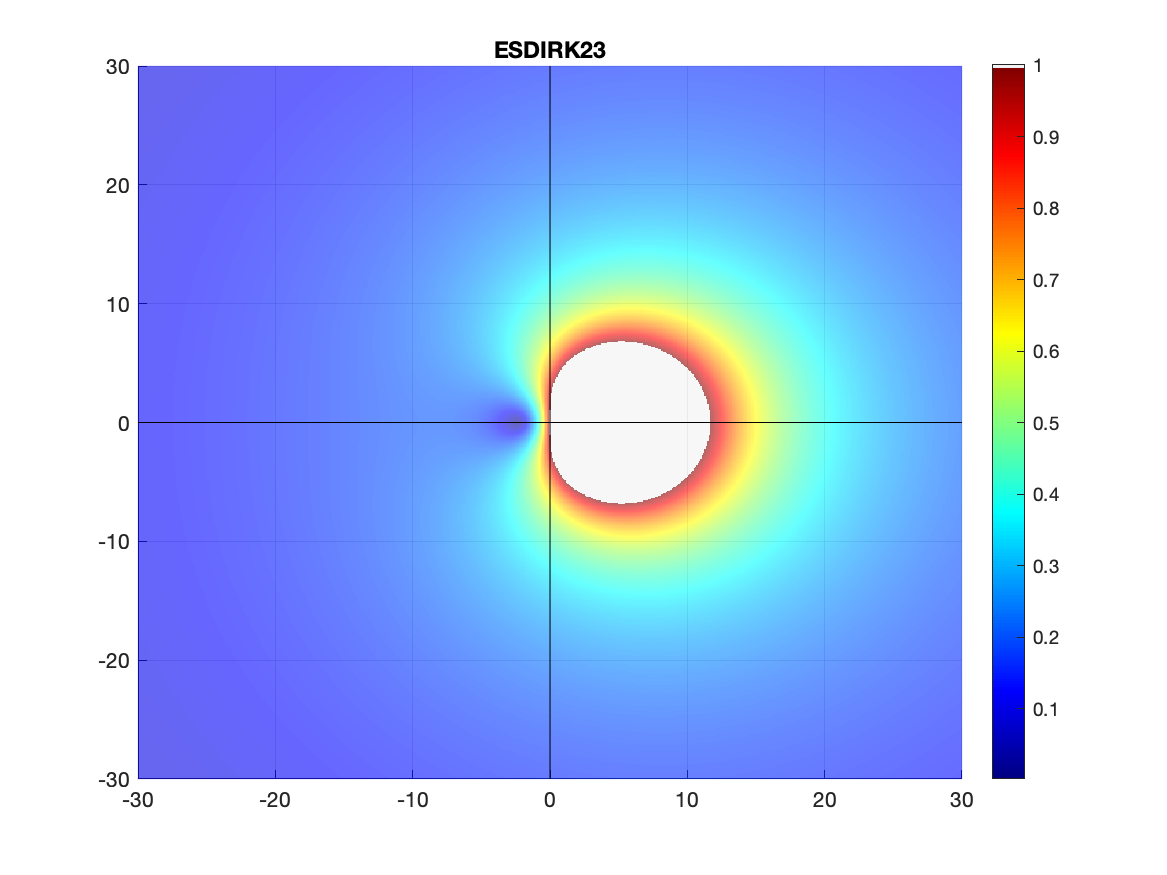
\includegraphics[width=\textwidth]{graphics/opg7/ESDIRK23-stability.png}
    \caption{Stability region of ESDIRK23, coloured area is stable}
    \label{fig7:stable}
\end{figure}

\section{Implementation of ESDIRK23 with adaptive time step}
Because ESDIRK23 is not an explicit method, we need to use an iterative method to determine each step. Specifically, we use a special form of inexact Newton, for stage 2 we want to solve

\begin{align}
    R_2(X_2) &= X_2 - h \gamma f(T_2,X_2) - \xi_2 = 0, \quad \xi_2 = x_n + h a_{21} f_1.
\end{align}
We do this by
\begin{align}
    f_2 &= f(T_2,X_2) \\
    J &= \frac{\partial f}{\partial x} (T_2,X_2) \\
    M &= I - h \gamma J \\
    M &= LU  \quad \text{LU: LU factorization of M} \\
    R_2 &= X_2 - h \gamma f(T_2,X_2) - \xi_2 \\
    LU \Delta X_2 &= -R_2 \quad \text{sole for $\Delta X_2$} \\
    X_2 :&= X_2 + \Delta X_2  \quad \text{Continue untill $||R_2|| < \varepsilon$}.
\end{align}

Notice that this is a specialized version that only works for ESDIRK23, and exploits structures in the tableau table to be more efficient.

For selecting the appropriate step size, we will use the \textit{predictive error controller} (PI controller). This means that we have

\begin{align}
    h_{n+1} &= \left ( \frac{h_n}{h_{n-1}}  \right )
    \left ( \frac{\varepsilon}{r_{n+1}} \right )^{\frac{1}{3}} 
    \left ( \frac{r_n}{r_{n+1}} \right )^{\frac{1}{3}} h_n
\end{align}
where (we use $||\cdot ||_\infty$)
\begin{align}
    r = \max_i \frac{|e_i|}{max \{AbsTol_i, |(x_n)_i| RelTol_i\} }
\end{align}

Listing \ref{lst7:esdirk} shows a Matlab implementation of a ESDIRK23 with adaptive time step.

\begin{lstlisting}[language=Matlab,caption=Implementation of ESDIRK23 with adaptive time step,label=lst7:esdirk]
function [Tout,Xout,Gout,info,stats] = ESDIRK(fun,jac,t0,tf,x0,h0,absTol,relTol,varargin)
%% ESDIRK23 Parameters 
%=========================================================================
% ESDIRK23 parameters
gamma = 1-1/sqrt(2);
a31 = (1-gamma)/2;
AT = [0 gamma a31;0 gamma a31;0 0 gamma];
c  = [0; 2*gamma; 1];
b  = AT(:,3);
bhat = [    (6*gamma-1)/(12*gamma); ...
    1/(12*gamma*(1-2*gamma)); ...
    (1-3*gamma)/(3*(1-2*gamma))    ];
d  = b-bhat;
p  = 2;
phat = 3;
s = 3;

% error and convergence controller
epsilon = 0.8;
tau = 0.1*epsilon; %0.005*epsilon;
itermax = 20;
ke0 = 1.0/phat;
ke1 = 1.0/phat;
ke2 = 1.0/phat;
alpharef = 0.3;
alphaJac = -0.2;
alphaLU  = -0.2;
hrmin = 0.01;
N = ceil((tf-t0)/hmin);
hs = zeros(2,N+1);
hrmax = 10;
%========================================================================
tspan = [t0 tf]; % carsten
info = struct(...
            'nStage',    s,       ... % carsten
            'absTol',    'dummy',  ... % carsten
            'relTol',    'dummy',  ... % carsten
            'iterMax',   itermax, ... % carsten
            'tspan',     tspan,   ... % carsten
            'nFun',      0, ...
            'nJac',      0, ...
            'nLU',       0, ...
            'nBack',     0, ...
            'nStep',     0, ...
            'nAccept',   0, ...
            'nFail',     0, ...
            'nDiverge',  0, ...
            'nSlowConv', 0);


        
%% Main ESDIRK Integrator
%========================================================================
nx = size(x0,1);
F = zeros(nx,s);
t = t0;
x = x0;
h = h0;

[F(:,1),g]  = feval(fun,t,x,varargin{:});
info.nFun = info.nFun+1;
[dfdx,dgdx] = feval(jac,t,x,varargin{:});
info.nJac = info.nJac+1;
FreshJacobian = true;
if (t+h)>tf
    h = tf-t;
end
hgamma = h*gamma;
dRdx = dgdx - hgamma*dfdx;
[L,U,pivot] = lu(dRdx,'vector');
info.nLU = info.nLU+1;
hLU = h;

FirstStep = true;
ConvergenceRestriction = false;
PreviousReject = false;
iter = zeros(1,s);

% Output
chunk = 100;
Tout = zeros(chunk,1);
Xout = zeros(chunk,nx);
Gout = zeros(chunk,nx); 

Tout(1,1) = t;
Xout(1,:) = x.';
Gout(1,:) = g.';

runs = 1;
while t<tf
    info.nStep = info.nStep+1;
    %=====================================================================
    % A step in the ESDIRK method
    i=1;   
    diverging = false;
    SlowConvergence = false; % carsten
    alpha = 0.0;
    Converged = true;
    while (i<s) && Converged
        % Stage i=2,...,s of the ESDIRK Method
        i=i+1;
        phi = g + F(:,1:i-1)*(h*AT(1:i-1,i));

        % Initial guess for the state
         if i==2
             dt = c(i)*h;
             G = g + dt*F(:,1);
             X = x + dgdx\(G-g);
         else
             dt = c(i)*h;
             G  = g + dt*F(:,1);
             X  = x + dgdx\(G-g);
         end
        T = t+dt;
            
        [F(:,i),G] = feval(fun,T,X,varargin{:});
        info.nFun = info.nFun+1;
        R = G - hgamma*F(:,i) - phi;
%        rNewton = norm(R./(absTol + abs(G).*relTol),2)/sqrt(nx);
        rNewton = norm(R./(absTol + abs(G).*relTol),inf);
        Converged = (rNewton < tau);
        %iter(i) = 0; % original, if uncomment then comment line 154: iter(:) = 0;
        % Newton Iterations
        while ~Converged && ~diverging && ~SlowConvergence%iter(i)<itermax
            iter(i) = iter(i)+1;
            dX = U\(L\(R(pivot,1)));
            info.nBack = info.nBack+1;
            X = X - dX;
            rNewtonOld = rNewton;
            [F(:,i),G] = feval(fun,T,X,varargin{:});
            info.nFun = info.nFun+1;
            R = G - hgamma*F(:,i) - phi;
%            rNewton = norm(R./(absTol + abs(G).*relTol),2)/sqrt(nx);
            rNewton = norm(R./(absTol + abs(G).*relTol),inf);
            alpha = max(alpha,rNewton/rNewtonOld);
            Converged = (rNewton < tau);
            diverging = (alpha >= 1);
            SlowConvergence = (iter(i) >= itermax); % carsten
            %SlowConvergence = (alpha >= 0.5); % carsten
            %if (iter(i) >= itermax), i, iter(i), Converged, diverging, pause, end % carsten
        end
        %diverging = (alpha >= 1); % original, if uncomment then comment line 142: diverging = (alpha >= 1)*i;
        diverging = (alpha >= 1)*i; % carsten, recording which stage is diverging
    end
    %if diverging, i, iter, pause, end
    nstep = info.nStep;
    stats.t(nstep) = t;
    stats.h(nstep) = h;
    stats.r(nstep) = NaN;
    stats.iter(nstep,:) = iter;
    stats.Converged(nstep) = Converged;
    stats.Diverged(nstep)  = diverging;
    stats.AcceptStep(nstep) = false;
    stats.SlowConv(nstep)  = SlowConvergence*i; % carsten, recording which stage is converging to slow (reaching maximum no. of iterations)
    iter(:) = 0; % carsten
    %=====================================================================
    % Error and Convergence Controller
    if Converged
        % Error estimation
        e = F*(h*d);
%        r = norm(e./(absTol + abs(G).*relTol),2)/sqrt(nx);
        r = norm(e./(absTol + abs(G).*relTol),inf);
        CurrentStepAccept = (r<=1.0);
        r = max(r,eps);
        stats.r(nstep) = r;
        % Step Length Controller
        if CurrentStepAccept
            stats.AcceptStep(nstep) = true;
            info.nAccept = info.nAccept+1;
            if FirstStep || PreviousReject || ConvergenceRestriction
                % Aymptotic step length controller
                hr = 0.75*(epsilon/r)^ke0; 
            else
                % Predictive controller
                s0 = (h/hacc);
                s1 = max(hrmin,min(hrmax,(racc/r)^ke1));
                s2 = max(hrmin,min(hrmax,(epsilon/r)^ke2));
                hr = 0.95*s0*s1*s2;
            end
            racc = r;
            hacc = h;
            FirstStep = false;
            PreviousReject = false;
            ConvergenceRestriction = false;
            
            % Next Step
            t = T;
            x = X;
            g = G;
            F(:,1) = F(:,s);            
            
        else % Reject current step
            info.nFail = info.nFail+1;
            if PreviousReject
                kest = log(r/rrej)/(log(h/hrej));
                kest = min(max(0.1,kest),phat);
                hr   = max(hrmin,min(hrmax,((epsilon/r)^(1/kest))));
            else
                hr = max(hrmin,min(hrmax,((epsilon/r)^ke0)));
            end
            rrej = r;
            hrej = h;
            PreviousReject = true;
        end
   
        % Convergence control
        halpha = (alpharef/alpha);
        if (alpha > alpharef)
            ConvergenceRestriction = true;
            if hr < halpha
                h = max(hrmin,min(hrmax,hr))*h;
            else
                h = max(hrmin,min(hrmax,halpha))*h;
            end
        else
            h = max(hrmin,min(hrmax,hr))*h;
        end
        h = max(1e-8,h);
        if (t+h) > tf
            h = tf-t;
        end
        
        % Jacobian Update Strategy
        FreshJacobian = false;
        if alpha > alphaJac
            [dfdx,dgdx] = feval(jac,t,x,varargin{:});
            info.nJac = info.nJac+1;
            FreshJacobian = true;
            hgamma = h*gamma;
            dRdx = dgdx - hgamma*dfdx; 
            [L,U,pivot] = lu(dRdx,'vector');
            info.nLU = info.nLU+1;
            hLU = h;
        elseif (abs(h-hLU)/hLU) > alphaLU 
            hgamma = h*gamma;
            dRdx = dgdx-hgamma*dfdx;
            [L,U,pivot] = lu(dRdx,'vector');
            info.nLU = info.nLU+1;
            hLU = h;
        end        
    else % not converged
        info.nFail=info.nFail+1;
        CurrentStepAccept = false;
        ConvergenceRestriction = true;
        if FreshJacobian && diverging
            h = max(0.5*hrmin,alpharef/alpha)*h;
            info.nDiverge = info.nDiverge+1;
        elseif FreshJacobian
            if alpha > alpharef
                h = max(0.5*hrmin,alpharef/alpha)*h;
            else
                h = 0.5*h;
            end
        end
        if ~FreshJacobian
            [dfdx,dgdx] = feval(jac,t,x,varargin{:});
            info.nJac = info.nJac+1;
            FreshJacobian = true;
        end
        hgamma = h*gamma;
        dRdx = dgdx - hgamma*dfdx;
        [L,U,pivot] = lu(dRdx,'vector');
        info.nLU = info.nLU+1;
        hLU = h;
    end
    
    %=====================================================================
    % Storage of variables for output
    
    if CurrentStepAccept
       nAccept = info.nAccept;
       if nAccept > length(Tout)
           Tout = [Tout; zeros(chunk,1)];
           Xout = [Xout; zeros(chunk,nx)];
           Gout = [Gout; zeros(chunk,nx)];
       end
       Tout(nAccept,1) = t;
       Xout(nAccept,:) = x.';
       Gout(nAccept,:) = g.';
    end

    
end
info.nSlowConv = length(find(stats.SlowConv)); % carsten
nAccept = info.nAccept;
Tout = Tout(1:nAccept,1);
Xout = Xout(1:nAccept,:);
Gout = Gout(1:nAccept,:);
\end{lstlisting}

\section{Test on Van der Pol problem and comparison with Matlab ODE solvers}
Now that we have an implementation of ESDIRK23 with adaptive step size we want to test it. To do so we look at the Van der Pol problem given by
\begin{align}
    \Ddot{x}(t) &= \mu (1-x(t)^2) \dot{x}(t) - x(t).
\end{align}
To solve the problem we must first re-write the problem as a system of first order differential equations. Luckily this is done easily and given by
\begin{align}
    \dot{x}_1(t) &= x_2(t) \\
    \dot{x}_2(t) &= \mu(1-x_1(t)^2) x_2(t) - x_1(t).
\end{align}

We will now test ESDIRK23 on the Van der Pol problem with $\mu = 3$ and $\mu = 20$. 

\subsection{Van der Pol, $\mu = 3$}
Figure \ref{fig7:mu3} shows the numerical solution to the Van der Pol problem with $\mu = 3$ for ESDIRK23 with adaptive time steps and $AbsTol=RelTol \in \{10^{-2}, 10^{-4}, 10^{-6}\}$, ODE45 and ODE15s. Notice also that for $Tol = 10^{-2}$ the only difference visible is again due to the relatively large steps that the algorithm takes in the "non-stiff" area. Otherwise, all tolerances seem to follow the ODE45/ODE15s solutions very well.

\begin{figure}[H]
    \centering
    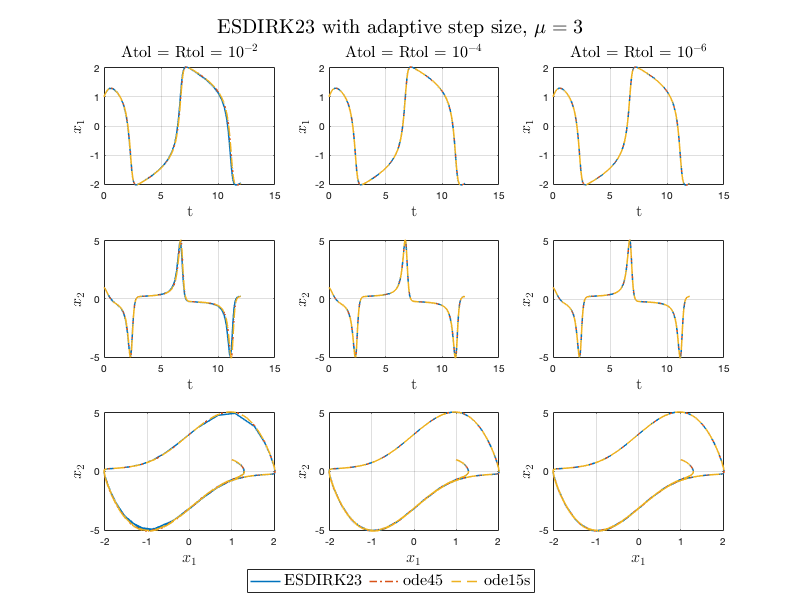
\includegraphics[width=\textwidth]{graphics/opg7/mu3.png}
    \caption{Solution to Van der Pol with $\mu = 3$ using adaptive step sizes}
    \label{fig7:mu3}
\end{figure}

Table \ref{tab7:mu3} shows the CPU time and number of function evaluations when solving the Van der Pol problem with $\mu = 3$ using different tolerances and Matlab ODE solvers. Notice that with $Tol = 10^{-2}$ the ESDIRK23 is relatively fast (slower than ODE45 but faster than ODE15s). Generally, it is very hard to tell the solutions curves apart just by looking at them. Even for the lowest tolerance, we get quite good results. What is interesting is the CPU time usage and number of function evaluations used at the different tolerances. For both explicit- and implicit Euler, we saw that the CPU time and function evaluations increased dramatically when we required higher accuracy, now this increase is not as pronounced. This demonstrates the power of higher order methods quite well.

\begin{table}[H]
    \centering
    \caption{CPU time and function evaluations of ESDIRK23 with adaptive time step and Matlab ODE solvers}
    \begin{tabular}{|c||c|c|c|c|c|c|} \hline
         \textbf{Method}    & $Tol = 10^{-2}$&   $Tol = 10^{-4}$ & $Tol = 10^{-6}$ & ODE45 & ODE15s     \\ \hline \hline 
         \textbf{Time}      & 0.0122 &   0.0167  &  0.0549 & 0.0046 & 0.0175   \\ \hline
         \textbf{Fun evals} & 517    &   1199  &    4488 & 1069 & 926  \\ \hline
    \end{tabular}
    \label{tab7:mu3}
\end{table}

Figure \ref{fig7:mu3_h} shows the used step sizes for the different tolerances. The red crosses mark whenever the step size controller failed to set the step size correctly, i.e., whenever the estimated (using the embedded error estimate) error was larger than the allowed maximum. Notice that the behaviour of all three tolerances are quite similar. Also notice that the step sizes does not vary nearly as much for the individual tolerances as previously seen (for explicit- and implicit Euler). Additionally, if we look at the difference in step sizes for the different tolerances, we see that in order to decrease the tolerance by a factor $10^4$, we do not even need to decrease the step size by a factor $10^2$. This is the true power of higher order methods! 

\begin{figure}[H]
    \centering
    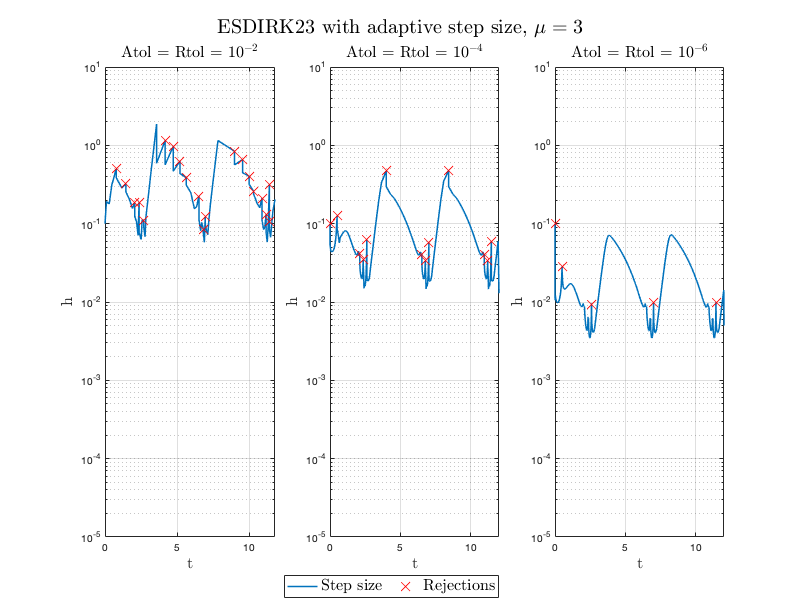
\includegraphics[width=\textwidth]{graphics/opg7/mu3_h.png}
    \caption{Step sizes when solving the Van der Pol with $\mu = 3$ at different tolerances}
    \label{fig7:mu3_h}
\end{figure}

\subsection{Van der Pol, $\mu = 20$}
The Van der Pol problem with $\mu = 20$ is a more complicated problem. The dynamics of the problem is largely defined by the $\mu$ parameter. In particular, the problem becomes more stiff when $\mu$ is increased.

Figure \ref{fig7:mu20} shows the numerical solution to the Van der Pol problem with $\mu = 20$ for ESDIRK23 with adaptive time steps and $AbsTol=RelTol \in \{10^{-2}, 10^{-4}, 10^{-6}\}$, ODE45 and ODE15s. Notice that for $Tol = 10^{-2}$ we see some difference in the plots. ESDIRK23 seem to be a bit to far \textit{ahead}, i.e., ESDIRK23 makes abrupt jump in values slightly before ODE45/ODE15s. The reason fore this is because it is to a large extend an implicit method. As such is has many characteristics of a right point method. In chapter 3, we saw the same sort of behaviour from implicit Euler.

\begin{figure}[H]
    \centering
    \includegraphics[width=\textwidth]{graphics/opg7/mu20.png}
    \caption{Solution to Van der Pol with $\mu = 20$ using adaptive step sizes}
    \label{fig7:mu20}
\end{figure}

Table \ref{tab7:mu20} shows that CPU time and number of function evaluations when solving the Van der Pol problem with $\mu = 20$ using different tolerances and Matlab ODE solvers. Notice that with $Tol = 10^{-2}$ the ESDIRK23 is very similar in speed to ODE45 (and faster than ODE15s). Once again notice that 100 times the accuracy does not require 100 times the CPU time or 100 times the function calls. This is because ESDIRK23 is a 2nd order method, i.e., the accuracy increase much faster than linear. 

\begin{table}[H]
    \centering
    \caption{CPU time and function evaluations of ESDIRK23 with adaptive time step and Matlab ODE solvers}
    \begin{tabular}{|c||c|c|c|c|c|c|} \hline
         \textbf{Method}    & $Tol = 10^{-2}$&   $Tol = 10^{-4}$ & $Tol = 10^{-6}$ & ODE45 & ODE15s     \\ \hline \hline 
         \textbf{Time}      & 0.0317   & 0.0445  &   0.1558 & 0.0386 & 0.0612   \\ \hline
         \textbf{Fun evals} &  1384     &   3383    &   12560 & 8461 & 2944  \\ \hline
    \end{tabular}
    \label{tab7:mu20}
\end{table}

Figure \ref{fig7:mu20_h} shows the used step sizes for the different tolerances. The red crosses mark whenever the step size controller failed to set the step size correctly, i.e., whenever the estimated error was larger than the allowed maximum. Notice that the behaviour of all three tolerances are not nearly as similar as previously seen. Notice that the step sizes does not vary nearly as much for the individual tolerances as previously seen (for explicit- and implicit Euler). In fact, we see that for a difference of a factor $10^4$ in accuracy, the difference is approximate a factor $10^2$ in step size. This is consistent with ESDIRK23 being a 2nd order method. 

\begin{figure}[H]
    \centering
    \includegraphics[width=\textwidth]{graphics/opg7/mu20_h.png}
    \caption{Step sizes when solving the Van der Pol with $\mu = 20$ at different tolerances}
    \label{fig7:mu20_h}
\end{figure}


\clearforchapter
\chapter{Conclusion}
We have now investigated the Van der Pol problems using different methods (and CSTR using DoPri54), and have a better understanding of which methods work better for different settings. For the Van der Pol problem, the choice of solution method becomes critical when we have large $\mu$-values. In these cases, the problem has stiff regions of rapid and large changes in the dynamics, making approximating the real solution difficult. The explicit adaptive Euler method was relatively slow due to many rejected states and low step size when better accuracy was required. It did not handle the Van der Pol problem very well. The implicit method had better convergence properties, but eventually required many more function evaluations, making it relatively slow. The explicit RK4 adaptive method was just as fast as the Matlab ODE solvers. It had a lower number of function evaluations than the implicit Euler. The DOPRI54 method behaves very much like the RK4, but is faster for the more stiff problem with $\mu = 20$. The ESDIRK23 method has almost no rejected states, but also requires more function evaluations. 

In the SDE problem, we saw  how the discrete points in the Van der Pol problem became extremely unpredictable for the second drift function (state dependent). For the independent state diffusion, the discrete points were more noisy, but a solution was better obtainable. This was the case for both explicit-explicit and implicit-explicit SDE methods. Again in the CSRT problem, the implicit-explicit method was more noisy in.

As a general conclusion, we have now looked at many different numerical algorithms, and have identified the pros and cons of each method. Every method has its own advantages and disadvantages, and the goal and budget for the implementation of the given problem is the "limiting factor". 

The key takeaway most be that whenever you need to use a scientific method for solving a differential equation it is really important to consider how your problem behaves and what methods is suitable. Generally speaking, you want to maximize you "bang-for-buck", such that you achieve the highest possible accuracy in the easiest way possible. For stiff problems, this requires good convergence properties of your method, hence you would prefer some implicit method. Otherwise, you would use a simple method that can give you your desired accuracy. If you need a good accuracy, it is therefore natural to select a higher order method. To maintain speed, you often want some kind of step control. This is why the standard choice of method is often the DoPri54, as is the case with ODE45 from Matlab.

All code in this report has been created in collaboration with Andreas Engly, s170303, and Anton Larsen, s174356. All code used for generation of plots etc is only given in the zip file handed in electronically. 




%\include{chapters/Introduction}
%\include{chapters/LongTitle}
%\blinddocument
%\include{chapters/Conclusion}

%\appendix
%%!TEX root = ../Thesis.tex
\chapter{An Appendix}
Lorem ipsum dolor sit amet, consectetur adipisicing elit, sed do eiusmod tempor incididunt ut labore et dolore magna aliqua. Ut enim ad minim veniam, quis nostrud exercitation ullamco laboris nisi ut aliquip ex ea commodo consequat. Duis aute irure dolor in reprehenderit in voluptate velit esse cillum dolore eu fugiat nulla pariatur. Excepteur sint occaecat cupidatat non proident, sunt in culpa qui officia deserunt mollit anim id est laborum.

\backmatter
\bibliographystyle{ieeetr}
\bibliography{bibliography/Bibliography.bib}

\end{document}
